\documentclass{book}
\usepackage[a4paper,top=2.5cm,bottom=2.5cm,left=2.5cm,right=2.5cm]{geometry}
\usepackage{makeidx}
\usepackage{natbib}
\usepackage{graphicx}
\usepackage{multicol}
\usepackage{float}
\usepackage{listings}
\usepackage{color}
\usepackage{ifthen}
\usepackage[table]{xcolor}
\usepackage{textcomp}
\usepackage{alltt}
\usepackage{ifpdf}
\ifpdf
\usepackage[pdftex,
            pagebackref=true,
            colorlinks=true,
            linkcolor=blue,
            unicode
           ]{hyperref}
\else
\usepackage[ps2pdf,
            pagebackref=true,
            colorlinks=true,
            linkcolor=blue,
            unicode
           ]{hyperref}
\usepackage{pspicture}
\fi
\usepackage[utf8]{inputenc}
\usepackage{mathptmx}
\usepackage[scaled=.90]{helvet}
\usepackage{courier}
\usepackage{sectsty}
\usepackage[titles]{tocloft}
\usepackage{doxygen}
\lstset{language=C++,inputencoding=utf8,basicstyle=\footnotesize,breaklines=true,breakatwhitespace=true,tabsize=8,numbers=left }
\makeindex
\setcounter{tocdepth}{3}
\renewcommand{\footrulewidth}{0.4pt}
\renewcommand{\familydefault}{\sfdefault}
\hfuzz=15pt
\setlength{\emergencystretch}{15pt}
\hbadness=750
\tolerance=750
\begin{document}
\hypersetup{pageanchor=false,citecolor=blue}
\begin{titlepage}
\vspace*{7cm}
\begin{center}
{\Large Mia\-:\-:Elementary }\\
\vspace*{1cm}
{\large Generated by Doxygen 1.8.1.1}\\
\vspace*{0.5cm}
{\small Sun Aug 12 2012 13:18:34}\\
\end{center}
\end{titlepage}
\clearemptydoublepage
\pagenumbering{roman}
\tableofcontents
\clearemptydoublepage
\pagenumbering{arabic}
\hypersetup{pageanchor=true,citecolor=blue}
\chapter{Namespace Index}
\section{Namespace List}
Here is a list of all documented namespaces with brief descriptions\-:\begin{DoxyCompactList}
\item\contentsline{section}{\hyperlink{namespacemia}{mia} \\*Just an umbralla namespace for elementary/storage manager etc }{\pageref{namespacemia}}{}
\item\contentsline{section}{\hyperlink{namespacemia_1_1elly}{mia\-::elly} \\*Namespace for Elementary }{\pageref{namespacemia_1_1elly}}{}
\item\contentsline{section}{\hyperlink{namespacemia_1_1elly_1_1alg}{mia\-::elly\-::alg} \\*Namespace for sampling algorithms }{\pageref{namespacemia_1_1elly_1_1alg}}{}
\item\contentsline{section}{\hyperlink{namespacemia_1_1elly_1_1dstruct}{mia\-::elly\-::dstruct} \\*Namespace for relations }{\pageref{namespacemia_1_1elly_1_1dstruct}}{}
\item\contentsline{section}{\hyperlink{namespacemia_1_1elly_1_1factors}{mia\-::elly\-::factors} \\*Namespace for registered factors }{\pageref{namespacemia_1_1elly_1_1factors}}{}
\item\contentsline{section}{\hyperlink{namespacemia_1_1elly_1_1mat}{mia\-::elly\-::mat} \\*Namespace for materialization strategies }{\pageref{namespacemia_1_1elly_1_1mat}}{}
\item\contentsline{section}{\hyperlink{namespacemia_1_1elly_1_1utils}{mia\-::elly\-::utils} \\*Utils used by elly }{\pageref{namespacemia_1_1elly_1_1utils}}{}
\item\contentsline{section}{\hyperlink{namespacemia_1_1sm}{mia\-::sm} \\*Namespace for storage manager }{\pageref{namespacemia_1_1sm}}{}
\end{DoxyCompactList}

\chapter{Class Index}
\section{Class Hierarchy}
This inheritance list is sorted roughly, but not completely, alphabetically\-:\begin{DoxyCompactList}
\item \contentsline{section}{mia\-:\-:elly\-:\-:dstruct\-:\-:Abstract\-Correlation\-Relation}{\pageref{classmia_1_1elly_1_1dstruct_1_1_abstract_correlation_relation}}{}
\begin{DoxyCompactList}
\item \contentsline{section}{mia\-:\-:elly\-:\-:dstruct\-:\-:Incremental\-Correlation\-Relation$<$ S\-T\-O\-R\-A\-G\-E, T\-Y\-P\-E $>$}{\pageref{classmia_1_1elly_1_1dstruct_1_1_incremental_correlation_relation}}{}
\item \contentsline{section}{mia\-:\-:elly\-:\-:dstruct\-:\-:Standard\-Correlation\-Relation$<$ S\-T\-O\-R\-A\-G\-E $>$}{\pageref{classmia_1_1elly_1_1dstruct_1_1_standard_correlation_relation}}{}
\end{DoxyCompactList}
\item \contentsline{section}{mia\-:\-:elly\-:\-:utils\-:\-:Config}{\pageref{classmia_1_1elly_1_1utils_1_1_config}}{}
\item \contentsline{section}{mia\-:\-:elly\-:\-:Elly}{\pageref{classmia_1_1elly_1_1_elly}}{}
\item \contentsline{section}{factor\-\_\-ldacount50}{\pageref{classfactor__ldacount50}}{}
\item \contentsline{section}{factor\-\_\-vidblock\-\_\-unigram}{\pageref{classfactor__vidblock__unigram}}{}
\item \contentsline{section}{mia\-:\-:elly\-:\-:utils\-:\-:Factor\-File\-Parser}{\pageref{classmia_1_1elly_1_1utils_1_1_factor_file_parser}}{}
\item \contentsline{section}{mia\-:\-:elly\-:\-:utils\-:\-:Factor\-Tuple}{\pageref{structmia_1_1elly_1_1utils_1_1_factor_tuple}}{}
\item \contentsline{section}{mia\-:\-:sm\-:\-:Int\-Pair}{\pageref{classmia_1_1sm_1_1_int_pair}}{}
\item \contentsline{section}{mia\-:\-:sm\-:\-:Ints\-Block}{\pageref{classmia_1_1sm_1_1_ints_block}}{}
\item \contentsline{section}{mia\-:\-:sm\-:\-:K\-V$<$ K\-E\-Y, V\-A\-L\-U\-E, M\-M, D\-I\-R\-E\-C\-T, R\-E\-P\-L\-A\-C\-E\-M\-E\-N\-T, H\-I\-N\-T $>$\-:\-:Iterator}{\pageref{classmia_1_1sm_1_1_k_v_3_01_k_e_y_00_01_v_a_l_u_e_00_01_m_m_00_01_d_i_r_e_c_t_00_01_r_e_p_l_a_c_6d8fd61b5ec60406ef5a5d4939c75a12}}{}
\item \contentsline{section}{mia\-:\-:sm\-:\-:K\-V$<$ int, V\-A\-L\-U\-E, M\-M, D\-I\-R\-E\-C\-T, R\-E\-P\-L\-A\-C\-E\-M\-E\-N\-T, D\-E\-N\-S\-E\-\_\-\-K\-E\-Y $>$\-:\-:Iterator}{\pageref{classmia_1_1sm_1_1_k_v_3_01int_00_01_v_a_l_u_e_00_01_m_m_00_01_d_i_r_e_c_t_00_01_r_e_p_l_a_c_e_m00136a9f08c6f99ce3723959776b6b87}}{}
\item \contentsline{section}{mia\-:\-:sm\-:\-:K\-V$<$ int, V\-A\-L\-U\-E, M\-M\-A\-P, D\-I\-R\-E\-C\-T, R\-E\-P\-L\-A\-C\-E\-M\-E\-N\-T, D\-E\-N\-S\-E\-\_\-\-K\-E\-Y $>$\-:\-:Iterator}{\pageref{classmia_1_1sm_1_1_k_v_3_01int_00_01_v_a_l_u_e_00_01_m_m_a_p_00_01_d_i_r_e_c_t_00_01_r_e_p_l_a_c777ddd58bcfb92c8593dd8ce3d26b512}}{}
\item \contentsline{section}{mia\-:\-:sm\-:\-:K\-V$<$ K\-E\-Y, V\-A\-L\-U\-E, S\-T\-O\-R\-A\-G\-E, B\-U\-F\-F\-E\-R, R\-E\-P\-L\-A\-C\-E\-M\-E\-N\-T, H\-I\-N\-T $>$\-:\-:Iterator}{\pageref{classmia_1_1sm_1_1_k_v_1_1_iterator}}{}
\item \contentsline{section}{mia\-:\-:sm\-:\-:K\-V$<$ K\-E\-Y, V\-A\-L\-U\-E, S\-T\-O\-R\-A\-G\-E, B\-U\-F\-F\-E\-R, R\-E\-P\-L\-A\-C\-E\-M\-E\-N\-T, H\-I\-N\-T $>$}{\pageref{classmia_1_1sm_1_1_k_v}}{}
\item \contentsline{section}{mia\-:\-:sm\-:\-:K\-V$<$ int, Ints\-Block, M\-M\-A\-P, D\-I\-R\-E\-C\-T, R\-E\-P\-L\-A\-C\-E\-M\-E\-N\-T, D\-E\-N\-S\-E\-\_\-\-K\-E\-Y $>$}{\pageref{classmia_1_1sm_1_1_k_v_3_01int_00_01_ints_block_00_01_m_m_a_p_00_01_d_i_r_e_c_t_00_01_r_e_p_l_a_e377a0951ed37be3b4316b2929369f72}}{}
\item \contentsline{section}{mia\-:\-:sm\-:\-:K\-V$<$ int, V\-A\-L\-U\-E, M\-M, D\-I\-R\-E\-C\-T, R\-E\-P\-L\-A\-C\-E\-M\-E\-N\-T, D\-E\-N\-S\-E\-\_\-\-K\-E\-Y $>$}{\pageref{classmia_1_1sm_1_1_k_v_3_01int_00_01_v_a_l_u_e_00_01_m_m_00_01_d_i_r_e_c_t_00_01_r_e_p_l_a_c_e_mff62509bd7761c1266e42e615210b694}}{}
\item \contentsline{section}{mia\-:\-:sm\-:\-:K\-V$<$ int, V\-A\-L\-U\-E, M\-M\-A\-P, D\-I\-R\-E\-C\-T, R\-E\-P\-L\-A\-C\-E\-M\-E\-N\-T, D\-E\-N\-S\-E\-\_\-\-K\-E\-Y $>$}{\pageref{classmia_1_1sm_1_1_k_v_3_01int_00_01_v_a_l_u_e_00_01_m_m_a_p_00_01_d_i_r_e_c_t_00_01_r_e_p_l_a_c808626285fb72e917596de806785defa}}{}
\item \contentsline{section}{mia\-:\-:sm\-:\-:K\-V$<$ K\-E\-Y, V\-A\-L\-U\-E, M\-M, D\-I\-R\-E\-C\-T, R\-E\-P\-L\-A\-C\-E\-M\-E\-N\-T, H\-I\-N\-T $>$}{\pageref{classmia_1_1sm_1_1_k_v_3_01_k_e_y_00_01_v_a_l_u_e_00_01_m_m_00_01_d_i_r_e_c_t_00_01_r_e_p_l_a_c_e_m_e_n_t_00_01_h_i_n_t_01_4}}{}
\item \contentsline{section}{mia\-:\-:sm\-:\-:K\-V$<$ K\-E\-Y, V\-A\-L\-U\-E, M\-M\-A\-P, D\-I\-R\-E\-C\-T, R\-E\-P\-L\-A\-C\-E\-M\-E\-N\-T, H\-I\-N\-T $>$}{\pageref{classmia_1_1sm_1_1_k_v_3_01_k_e_y_00_01_v_a_l_u_e_00_01_m_m_a_p_00_01_d_i_r_e_c_t_00_01_r_e_p_l_2c35447e93d2a07c32ca67010a09264b}}{}
\item \contentsline{section}{mia\-:\-:elly\-:\-:mat\-:\-:Materialization\-\_\-lazy}{\pageref{classmia_1_1elly_1_1mat_1_1_materialization__lazy}}{}
\item \contentsline{section}{mia\-:\-:elly\-:\-:Sample\-Input}{\pageref{classmia_1_1elly_1_1_sample_input}}{}
\item \contentsline{section}{mia\-:\-:elly\-:\-:Sample\-Task}{\pageref{classmia_1_1elly_1_1_sample_task}}{}
\item \contentsline{section}{mia\-:\-:sm\-:\-:Slotted\-Page}{\pageref{classmia_1_1sm_1_1_slotted_page}}{}
\item \contentsline{section}{tests}{\pageref{structtests}}{}
\item \contentsline{section}{mia\-:\-:elly\-:\-:utils\-:\-:Timer}{\pageref{classmia_1_1elly_1_1utils_1_1_timer}}{}
\item \contentsline{section}{mia\-:\-:elly\-:\-:dstruct\-:\-:Variable\-Assignment\-Relation}{\pageref{classmia_1_1elly_1_1dstruct_1_1_variable_assignment_relation}}{}
\item \contentsline{section}{mia\-:\-:elly\-:\-:dstruct\-:\-:Variable\-Factor\-Relation}{\pageref{classmia_1_1elly_1_1dstruct_1_1_variable_factor_relation}}{}
\item \contentsline{section}{mia\-:\-:elly\-:\-:dstruct\-:\-:Variable\-Tally\-Relation}{\pageref{classmia_1_1elly_1_1dstruct_1_1_variable_tally_relation}}{}
\item \contentsline{section}{mia\-:\-:elly\-:\-:dstruct\-:\-:Variable\-Training\-Relation}{\pageref{classmia_1_1elly_1_1dstruct_1_1_variable_training_relation}}{}
\end{DoxyCompactList}

\chapter{Class Index}
\section{Class List}
Here are the classes, structs, unions and interfaces with brief descriptions\-:\begin{DoxyCompactList}
\item\contentsline{section}{\hyperlink{classmia_1_1elly_1_1dstruct_1_1_abstract_correlation_relation}{mia\-::elly\-::dstruct\-::\-Abstract\-Correlation\-Relation} \\*Abstract class for unifying \hyperlink{classmia_1_1elly_1_1dstruct_1_1_standard_correlation_relation}{mia\-::elly\-::dstruct\-::\-Standard\-Correlation\-Relation} and \hyperlink{classmia_1_1elly_1_1dstruct_1_1_incremental_correlation_relation}{mia\-::elly\-::dstruct\-::\-Incremental\-Correlation\-Relation} }{\pageref{classmia_1_1elly_1_1dstruct_1_1_abstract_correlation_relation}}{}
\item\contentsline{section}{\hyperlink{classmia_1_1elly_1_1utils_1_1_config}{mia\-::elly\-::utils\-::\-Config} \\*Configurations to run elly }{\pageref{classmia_1_1elly_1_1utils_1_1_config}}{}
\item\contentsline{section}{\hyperlink{classmia_1_1elly_1_1_elly}{mia\-::elly\-::\-Elly} }{\pageref{classmia_1_1elly_1_1_elly}}{}
\item\contentsline{section}{\hyperlink{classfactor__ldacount50}{factor\-\_\-ldacount50} \\*Factor class for L\-D\-A ($<$50 topics) }{\pageref{classfactor__ldacount50}}{}
\item\contentsline{section}{\hyperlink{classfactor__vidblock__unigram}{factor\-\_\-vidblock\-\_\-unigram} \\*Factor class for general factor relies on V\-I\-Ds }{\pageref{classfactor__vidblock__unigram}}{}
\item\contentsline{section}{\hyperlink{classmia_1_1elly_1_1utils_1_1_factor_file_parser}{mia\-::elly\-::utils\-::\-Factor\-File\-Parser} \\*Class that contains a set of relations and load them }{\pageref{classmia_1_1elly_1_1utils_1_1_factor_file_parser}}{}
\item\contentsline{section}{\hyperlink{structmia_1_1elly_1_1utils_1_1_factor_tuple}{mia\-::elly\-::utils\-::\-Factor\-Tuple} }{\pageref{structmia_1_1elly_1_1utils_1_1_factor_tuple}}{}
\item\contentsline{section}{\hyperlink{classmia_1_1elly_1_1dstruct_1_1_incremental_correlation_relation}{mia\-::elly\-::dstruct\-::\-Incremental\-Correlation\-Relation$<$ S\-T\-O\-R\-A\-G\-E, T\-Y\-P\-E $>$} \\*Correlation relation in which each factor contains a fixed-\/size state }{\pageref{classmia_1_1elly_1_1dstruct_1_1_incremental_correlation_relation}}{}
\item\contentsline{section}{\hyperlink{classmia_1_1sm_1_1_int_pair}{mia\-::sm\-::\-Int\-Pair} \\*Pair of integer }{\pageref{classmia_1_1sm_1_1_int_pair}}{}
\item\contentsline{section}{\hyperlink{classmia_1_1sm_1_1_ints_block}{mia\-::sm\-::\-Ints\-Block} \\*A block of integer. Used as a container for variance length object }{\pageref{classmia_1_1sm_1_1_ints_block}}{}
\item\contentsline{section}{\hyperlink{classmia_1_1sm_1_1_k_v_3_01_k_e_y_00_01_v_a_l_u_e_00_01_m_m_00_01_d_i_r_e_c_t_00_01_r_e_p_l_a_c_6d8fd61b5ec60406ef5a5d4939c75a12}{mia\-::sm\-::\-K\-V$<$ K\-E\-Y, V\-A\-L\-U\-E, M\-M, D\-I\-R\-E\-C\-T, R\-E\-P\-L\-A\-C\-E\-M\-E\-N\-T, H\-I\-N\-T $>$\-::\-Iterator} }{\pageref{classmia_1_1sm_1_1_k_v_3_01_k_e_y_00_01_v_a_l_u_e_00_01_m_m_00_01_d_i_r_e_c_t_00_01_r_e_p_l_a_c_6d8fd61b5ec60406ef5a5d4939c75a12}}{}
\item\contentsline{section}{\hyperlink{classmia_1_1sm_1_1_k_v_3_01int_00_01_v_a_l_u_e_00_01_m_m_00_01_d_i_r_e_c_t_00_01_r_e_p_l_a_c_e_m00136a9f08c6f99ce3723959776b6b87}{mia\-::sm\-::\-K\-V$<$ int, V\-A\-L\-U\-E, M\-M, D\-I\-R\-E\-C\-T, R\-E\-P\-L\-A\-C\-E\-M\-E\-N\-T, D\-E\-N\-S\-E\-\_\-\-K\-E\-Y $>$\-::\-Iterator} }{\pageref{classmia_1_1sm_1_1_k_v_3_01int_00_01_v_a_l_u_e_00_01_m_m_00_01_d_i_r_e_c_t_00_01_r_e_p_l_a_c_e_m00136a9f08c6f99ce3723959776b6b87}}{}
\item\contentsline{section}{\hyperlink{classmia_1_1sm_1_1_k_v_3_01int_00_01_v_a_l_u_e_00_01_m_m_a_p_00_01_d_i_r_e_c_t_00_01_r_e_p_l_a_c777ddd58bcfb92c8593dd8ce3d26b512}{mia\-::sm\-::\-K\-V$<$ int, V\-A\-L\-U\-E, M\-M\-A\-P, D\-I\-R\-E\-C\-T, R\-E\-P\-L\-A\-C\-E\-M\-E\-N\-T, D\-E\-N\-S\-E\-\_\-\-K\-E\-Y $>$\-::\-Iterator} }{\pageref{classmia_1_1sm_1_1_k_v_3_01int_00_01_v_a_l_u_e_00_01_m_m_a_p_00_01_d_i_r_e_c_t_00_01_r_e_p_l_a_c777ddd58bcfb92c8593dd8ce3d26b512}}{}
\item\contentsline{section}{\hyperlink{classmia_1_1sm_1_1_k_v_1_1_iterator}{mia\-::sm\-::\-K\-V$<$ K\-E\-Y, V\-A\-L\-U\-E, S\-T\-O\-R\-A\-G\-E, B\-U\-F\-F\-E\-R, R\-E\-P\-L\-A\-C\-E\-M\-E\-N\-T, H\-I\-N\-T $>$\-::\-Iterator} \\*\hyperlink{classmia_1_1sm_1_1_k_v_1_1_iterator}{Iterator} for key-\/value store }{\pageref{classmia_1_1sm_1_1_k_v_1_1_iterator}}{}
\item\contentsline{section}{\hyperlink{classmia_1_1sm_1_1_k_v}{mia\-::sm\-::\-K\-V$<$ K\-E\-Y, V\-A\-L\-U\-E, S\-T\-O\-R\-A\-G\-E, B\-U\-F\-F\-E\-R, R\-E\-P\-L\-A\-C\-E\-M\-E\-N\-T, H\-I\-N\-T $>$} \\*Interface of key-\/value storage }{\pageref{classmia_1_1sm_1_1_k_v}}{}
\item\contentsline{section}{\hyperlink{classmia_1_1sm_1_1_k_v_3_01int_00_01_ints_block_00_01_m_m_a_p_00_01_d_i_r_e_c_t_00_01_r_e_p_l_a_e377a0951ed37be3b4316b2929369f72}{mia\-::sm\-::\-K\-V$<$ int, Ints\-Block, M\-M\-A\-P, D\-I\-R\-E\-C\-T, R\-E\-P\-L\-A\-C\-E\-M\-E\-N\-T, D\-E\-N\-S\-E\-\_\-\-K\-E\-Y $>$} \\*Key-\/value store for dense int key, variable length value, in M\-M\-A\-P }{\pageref{classmia_1_1sm_1_1_k_v_3_01int_00_01_ints_block_00_01_m_m_a_p_00_01_d_i_r_e_c_t_00_01_r_e_p_l_a_e377a0951ed37be3b4316b2929369f72}}{}
\item\contentsline{section}{\hyperlink{classmia_1_1sm_1_1_k_v_3_01int_00_01_v_a_l_u_e_00_01_m_m_00_01_d_i_r_e_c_t_00_01_r_e_p_l_a_c_e_mff62509bd7761c1266e42e615210b694}{mia\-::sm\-::\-K\-V$<$ int, V\-A\-L\-U\-E, M\-M, D\-I\-R\-E\-C\-T, R\-E\-P\-L\-A\-C\-E\-M\-E\-N\-T, D\-E\-N\-S\-E\-\_\-\-K\-E\-Y $>$} \\*Key value store for dense int key and arbitrary value type in main memory }{\pageref{classmia_1_1sm_1_1_k_v_3_01int_00_01_v_a_l_u_e_00_01_m_m_00_01_d_i_r_e_c_t_00_01_r_e_p_l_a_c_e_mff62509bd7761c1266e42e615210b694}}{}
\item\contentsline{section}{\hyperlink{classmia_1_1sm_1_1_k_v_3_01int_00_01_v_a_l_u_e_00_01_m_m_a_p_00_01_d_i_r_e_c_t_00_01_r_e_p_l_a_c808626285fb72e917596de806785defa}{mia\-::sm\-::\-K\-V$<$ int, V\-A\-L\-U\-E, M\-M\-A\-P, D\-I\-R\-E\-C\-T, R\-E\-P\-L\-A\-C\-E\-M\-E\-N\-T, D\-E\-N\-S\-E\-\_\-\-K\-E\-Y $>$} \\*Key value store for dense int key and arbitrary value in M\-M\-A\-P }{\pageref{classmia_1_1sm_1_1_k_v_3_01int_00_01_v_a_l_u_e_00_01_m_m_a_p_00_01_d_i_r_e_c_t_00_01_r_e_p_l_a_c808626285fb72e917596de806785defa}}{}
\item\contentsline{section}{\hyperlink{classmia_1_1sm_1_1_k_v_3_01_k_e_y_00_01_v_a_l_u_e_00_01_m_m_00_01_d_i_r_e_c_t_00_01_r_e_p_l_a_c_e_m_e_n_t_00_01_h_i_n_t_01_4}{mia\-::sm\-::\-K\-V$<$ K\-E\-Y, V\-A\-L\-U\-E, M\-M, D\-I\-R\-E\-C\-T, R\-E\-P\-L\-A\-C\-E\-M\-E\-N\-T, H\-I\-N\-T $>$} \\*Key-\/value store for arbitary key and value type in main memory }{\pageref{classmia_1_1sm_1_1_k_v_3_01_k_e_y_00_01_v_a_l_u_e_00_01_m_m_00_01_d_i_r_e_c_t_00_01_r_e_p_l_a_c_e_m_e_n_t_00_01_h_i_n_t_01_4}}{}
\item\contentsline{section}{\hyperlink{classmia_1_1sm_1_1_k_v_3_01_k_e_y_00_01_v_a_l_u_e_00_01_m_m_a_p_00_01_d_i_r_e_c_t_00_01_r_e_p_l_2c35447e93d2a07c32ca67010a09264b}{mia\-::sm\-::\-K\-V$<$ K\-E\-Y, V\-A\-L\-U\-E, M\-M\-A\-P, D\-I\-R\-E\-C\-T, R\-E\-P\-L\-A\-C\-E\-M\-E\-N\-T, H\-I\-N\-T $>$} }{\pageref{classmia_1_1sm_1_1_k_v_3_01_k_e_y_00_01_v_a_l_u_e_00_01_m_m_a_p_00_01_d_i_r_e_c_t_00_01_r_e_p_l_2c35447e93d2a07c32ca67010a09264b}}{}
\item\contentsline{section}{\hyperlink{classmia_1_1elly_1_1mat_1_1_materialization__lazy}{mia\-::elly\-::mat\-::\-Materialization\-\_\-lazy} \\*Class for lazy materialization. See T\-R for details }{\pageref{classmia_1_1elly_1_1mat_1_1_materialization__lazy}}{}
\item\contentsline{section}{\hyperlink{classmia_1_1elly_1_1_sample_input}{mia\-::elly\-::\-Sample\-Input} \\*The class for a sample task of one variable }{\pageref{classmia_1_1elly_1_1_sample_input}}{}
\item\contentsline{section}{\hyperlink{classmia_1_1elly_1_1_sample_task}{mia\-::elly\-::\-Sample\-Task} \\*A sample task for Elementary }{\pageref{classmia_1_1elly_1_1_sample_task}}{}
\item\contentsline{section}{\hyperlink{classmia_1_1sm_1_1_slotted_page}{mia\-::sm\-::\-Slotted\-Page} \\*Slotted page, with each record a \hyperlink{classmia_1_1sm_1_1_ints_block}{mia\-::sm\-::\-Ints\-Block} }{\pageref{classmia_1_1sm_1_1_slotted_page}}{}
\item\contentsline{section}{\hyperlink{classmia_1_1elly_1_1dstruct_1_1_standard_correlation_relation}{mia\-::elly\-::dstruct\-::\-Standard\-Correlation\-Relation$<$ S\-T\-O\-R\-A\-G\-E $>$} \\*Correlation relation in which each factor contains a list of variable I\-Ds }{\pageref{classmia_1_1elly_1_1dstruct_1_1_standard_correlation_relation}}{}
\item\contentsline{section}{\hyperlink{structtests}{tests} }{\pageref{structtests}}{}
\item\contentsline{section}{\hyperlink{classmia_1_1elly_1_1utils_1_1_timer}{mia\-::elly\-::utils\-::\-Timer} }{\pageref{classmia_1_1elly_1_1utils_1_1_timer}}{}
\item\contentsline{section}{\hyperlink{classmia_1_1elly_1_1dstruct_1_1_variable_assignment_relation}{mia\-::elly\-::dstruct\-::\-Variable\-Assignment\-Relation} \\*Variable assignment relation, which maps V\-I\-D to its current assignment }{\pageref{classmia_1_1elly_1_1dstruct_1_1_variable_assignment_relation}}{}
\item\contentsline{section}{\hyperlink{classmia_1_1elly_1_1dstruct_1_1_variable_factor_relation}{mia\-::elly\-::dstruct\-::\-Variable\-Factor\-Relation} \\*Variable factor relation which maps each variable to the set of factors }{\pageref{classmia_1_1elly_1_1dstruct_1_1_variable_factor_relation}}{}
\item\contentsline{section}{\hyperlink{classmia_1_1elly_1_1dstruct_1_1_variable_tally_relation}{mia\-::elly\-::dstruct\-::\-Variable\-Tally\-Relation} \\*Variable tally relation which maps a variable to the int block contains tally info }{\pageref{classmia_1_1elly_1_1dstruct_1_1_variable_tally_relation}}{}
\item\contentsline{section}{\hyperlink{classmia_1_1elly_1_1dstruct_1_1_variable_training_relation}{mia\-::elly\-::dstruct\-::\-Variable\-Training\-Relation} \\*Variable training relation which maps a variable to its value in training data }{\pageref{classmia_1_1elly_1_1dstruct_1_1_variable_training_relation}}{}
\end{DoxyCompactList}

\chapter{Namespace Documentation}
\hypertarget{namespacemia}{\section{mia Namespace Reference}
\label{namespacemia}\index{mia@{mia}}
}


Just an umbralla namespace for elementary/storage manager etc.  


\subsection*{Namespaces}
\begin{DoxyCompactItemize}
\item 
namespace \hyperlink{namespacemia_1_1elly}{elly}
\begin{DoxyCompactList}\small\item\em Namespace for Elementary. \end{DoxyCompactList}\item 
namespace \hyperlink{namespacemia_1_1sm}{sm}
\begin{DoxyCompactList}\small\item\em Namespace for storage manager. \end{DoxyCompactList}\end{DoxyCompactItemize}


\subsection{Detailed Description}
Just an umbralla namespace for elementary/storage manager etc. Namespace of Mia. 
\hypertarget{namespacemia_1_1elly}{\section{mia\-:\-:elly Namespace Reference}
\label{namespacemia_1_1elly}\index{mia\-::elly@{mia\-::elly}}
}
\subsection*{Namespaces}
\begin{DoxyCompactItemize}
\item 
namespace \hyperlink{namespacemia_1_1elly_1_1alg}{alg}
\item 
namespace \hyperlink{namespacemia_1_1elly_1_1dstruct}{dstruct}
\item 
namespace \hyperlink{namespacemia_1_1elly_1_1factors}{factors}
\item 
namespace \hyperlink{namespacemia_1_1elly_1_1mat}{mat}
\item 
namespace \hyperlink{namespacemia_1_1elly_1_1utils}{utils}
\end{DoxyCompactItemize}
\subsection*{Classes}
\begin{DoxyCompactItemize}
\item 
class \hyperlink{classmia_1_1elly_1_1_sample_task}{Sample\-Task}
\item 
class \hyperlink{classmia_1_1elly_1_1_elly}{Elly}
\item 
class \hyperlink{classmia_1_1elly_1_1_sample_input}{Sample\-Input}
\end{DoxyCompactItemize}
\subsection*{Functions}
\begin{DoxyCompactItemize}
\item 
\hypertarget{namespacemia_1_1elly_a4f35fa786e9e6f482f3881b8c6e66e1a}{void $\ast$ {\bfseries mapper\-\_\-sample} (void $\ast$sample\-Task)}\label{namespacemia_1_1elly_a4f35fa786e9e6f482f3881b8c6e66e1a}

\end{DoxyCompactItemize}


\subsection{Detailed Description}
Namespace of \hyperlink{classmia_1_1elly_1_1_elly}{Elly} -- the inference engine. 
\hypertarget{namespacemia_1_1elly_1_1alg}{\section{mia\-:\-:elly\-:\-:alg Namespace Reference}
\label{namespacemia_1_1elly_1_1alg}\index{mia\-::elly\-::alg@{mia\-::elly\-::alg}}
}
\subsection*{Functions}
\begin{DoxyCompactItemize}
\item 
int \hyperlink{namespacemia_1_1elly_1_1alg_ab8c9dff4bb66e3a9615525662a8f4af0}{Shuffle} (\hyperlink{classmia_1_1elly_1_1_sample_input}{mia\-::elly\-::\-Sample\-Input} \&sample\-Input)
\item 
int \hyperlink{namespacemia_1_1elly_1_1alg_a19a80aed51e58ec0661bd869af34c7d6}{Gibbs\-Sampling} (\hyperlink{classmia_1_1elly_1_1_sample_input}{mia\-::elly\-::\-Sample\-Input} \&sample\-Input, int thread\-\_\-id, std\-::vector$<$ double $>$ $\ast$vector\-\_\-pool, bool is\-\_\-log\-\_\-system=true)
\end{DoxyCompactItemize}


\subsection{Detailed Description}
Namespace for sampling algorithms. 

\subsection{Function Documentation}
\hypertarget{namespacemia_1_1elly_1_1alg_a19a80aed51e58ec0661bd869af34c7d6}{\index{mia\-::elly\-::alg@{mia\-::elly\-::alg}!Gibbs\-Sampling@{Gibbs\-Sampling}}
\index{Gibbs\-Sampling@{Gibbs\-Sampling}!mia::elly::alg@{mia\-::elly\-::alg}}
\subsubsection[{Gibbs\-Sampling}]{\setlength{\rightskip}{0pt plus 5cm}int mia\-::elly\-::alg\-::\-Gibbs\-Sampling (
\begin{DoxyParamCaption}
\item[{{\bf mia\-::elly\-::\-Sample\-Input} \&}]{sample\-Input, }
\item[{int}]{thread\-\_\-id, }
\item[{std\-::vector$<$ double $>$ $\ast$}]{vector\-\_\-pool, }
\item[{bool}]{is\-\_\-log\-\_\-system = {\ttfamily true}}
\end{DoxyParamCaption}
)}}\label{namespacemia_1_1elly_1_1alg_a19a80aed51e58ec0661bd869af34c7d6}
Sample new assignment of a \hyperlink{classmia_1_1elly_1_1_sample_input}{mia\-::elly\-::\-Sample\-Input} object. Also, \hyperlink{classmia_1_1elly_1_1_sample_input_a0016cf98d8b1a50f42a5b85e091e61f9}{mia\-::elly\-::\-Sample\-Input\-::log\-\_\-improve\-\_\-ratio} will be filled in by the improvement of probability of new assignment compared with original assignment. If \hyperlink{classmia_1_1elly_1_1_sample_input}{mia\-::elly\-::\-Sample\-Input} contains training data (mia\-::elly\-::sample\-Input\-::vtrain$>$0), also update weights by calling gradient function for each factor.


\begin{DoxyParams}{Parameters}
{\em sample\-Input} & reference to a sample task \\
\hline
{\em thread\-\_\-id} & a number in 0$\sim$\#threads \\
\hline
{\em vector\-\_\-pool} & object pool to avoid re-\/allocate of vectors, vector\-\_\-pool\mbox{[}thread\-\_\-id\mbox{]} is a vector. \\
\hline
{\em is\-\_\-log\-\_\-system} & true if all factors return in log scale, otherwise linear scale (weight vs. exp(weight) ).\\
\hline
\end{DoxyParams}
\begin{DoxyReturn}{Returns}
assigned value to \hyperlink{classmia_1_1elly_1_1_sample_input}{mia\-::elly\-::\-Sample\-Input}. Also the
\end{DoxyReturn}
\begin{DoxySeeAlso}{See also}
\hyperlink{classmia_1_1elly_1_1_sample_input}{mia\-::elly\-::\-Sample\-Input} 
\end{DoxySeeAlso}
\hypertarget{namespacemia_1_1elly_1_1alg_ab8c9dff4bb66e3a9615525662a8f4af0}{\index{mia\-::elly\-::alg@{mia\-::elly\-::alg}!Shuffle@{Shuffle}}
\index{Shuffle@{Shuffle}!mia::elly::alg@{mia\-::elly\-::alg}}
\subsubsection[{Shuffle}]{\setlength{\rightskip}{0pt plus 5cm}int mia\-::elly\-::alg\-::\-Shuffle (
\begin{DoxyParamCaption}
\item[{{\bf mia\-::elly\-::\-Sample\-Input} \&}]{sample\-Input}
\end{DoxyParamCaption}
)}}\label{namespacemia_1_1elly_1_1alg_ab8c9dff4bb66e3a9615525662a8f4af0}
Randomly shuffle the assignment of a \hyperlink{classmia_1_1elly_1_1_sample_input}{mia\-::elly\-::\-Sample\-Input} object.


\begin{DoxyParams}{Parameters}
{\em sample\-Input} & reference to a sample task\\
\hline
\end{DoxyParams}
\begin{DoxyReturn}{Returns}
assigned value to \hyperlink{classmia_1_1elly_1_1_sample_input}{mia\-::elly\-::\-Sample\-Input}.
\end{DoxyReturn}
\begin{DoxySeeAlso}{See also}
\hyperlink{classmia_1_1elly_1_1_sample_input}{mia\-::elly\-::\-Sample\-Input} 
\end{DoxySeeAlso}

\hypertarget{namespacemia_1_1elly_1_1dstruct}{\section{mia\-:\-:elly\-:\-:dstruct Namespace Reference}
\label{namespacemia_1_1elly_1_1dstruct}\index{mia\-::elly\-::dstruct@{mia\-::elly\-::dstruct}}
}
\subsection*{Classes}
\begin{DoxyCompactItemize}
\item 
class \hyperlink{classmia_1_1elly_1_1dstruct_1_1_abstract_correlation_relation}{Abstract\-Correlation\-Relation}
\item 
class \hyperlink{classmia_1_1elly_1_1dstruct_1_1_incremental_correlation_relation}{Incremental\-Correlation\-Relation}
\item 
class \hyperlink{classmia_1_1elly_1_1dstruct_1_1_standard_correlation_relation}{Standard\-Correlation\-Relation}
\item 
class \hyperlink{classmia_1_1elly_1_1dstruct_1_1_variable_assignment_relation}{Variable\-Assignment\-Relation}
\item 
class \hyperlink{classmia_1_1elly_1_1dstruct_1_1_variable_factor_relation}{Variable\-Factor\-Relation}
\item 
class \hyperlink{classmia_1_1elly_1_1dstruct_1_1_variable_tally_relation}{Variable\-Tally\-Relation}
\item 
class \hyperlink{classmia_1_1elly_1_1dstruct_1_1_variable_training_relation}{Variable\-Training\-Relation}
\end{DoxyCompactItemize}


\subsection{Detailed Description}
Namespace for relations. 
\hypertarget{namespacemia_1_1elly_1_1factors}{\section{mia\-:\-:elly\-:\-:factors Namespace Reference}
\label{namespacemia_1_1elly_1_1factors}\index{mia\-::elly\-::factors@{mia\-::elly\-::factors}}
}


Namespace for registered factors.  


\subsection*{Functions}
\begin{DoxyCompactItemize}
\item 
void \hyperlink{namespacemia_1_1elly_1_1factors_a1e408cecf7e7bdba69d9ce1bb78b5ec0}{register\-\_\-potentials} ()
\item 
void \hyperlink{namespacemia_1_1elly_1_1factors_a3b2e7562146e4d807ec2855fccbc8282}{register\-\_\-updates} ()
\item 
{\footnotesize template$<$mia\-::sm\-::\-K\-V\-\_\-\-Storage S\-T\-O\-R\-A\-G\-E$>$ }\\\hyperlink{classmia_1_1elly_1_1dstruct_1_1_abstract_correlation_relation}{mia\-::elly\-::dstruct\-::\-Abstract\-Correlation\-Relation} $\ast$ \hyperlink{namespacemia_1_1elly_1_1factors_a52975b837a6ff295ebe531bca52168f1}{get\-\_\-correlation\-\_\-relation} (int function\-\_\-id)
\end{DoxyCompactItemize}


\subsection{Detailed Description}
Namespace for registered factors. 

\subsection{Function Documentation}
\hypertarget{namespacemia_1_1elly_1_1factors_a52975b837a6ff295ebe531bca52168f1}{\index{mia\-::elly\-::factors@{mia\-::elly\-::factors}!get\-\_\-correlation\-\_\-relation@{get\-\_\-correlation\-\_\-relation}}
\index{get\-\_\-correlation\-\_\-relation@{get\-\_\-correlation\-\_\-relation}!mia::elly::factors@{mia\-::elly\-::factors}}
\subsubsection[{get\-\_\-correlation\-\_\-relation}]{\setlength{\rightskip}{0pt plus 5cm}template$<$mia\-::sm\-::\-K\-V\-\_\-\-Storage S\-T\-O\-R\-A\-G\-E$>$ {\bf mia\-::elly\-::dstruct\-::\-Abstract\-Correlation\-Relation}$\ast$ mia\-::elly\-::factors\-::get\-\_\-correlation\-\_\-relation (
\begin{DoxyParamCaption}
\item[{int}]{function\-\_\-id}
\end{DoxyParamCaption}
)}}\label{namespacemia_1_1elly_1_1factors_a52975b837a6ff295ebe531bca52168f1}
Given a factor\-I\-D, return a correlation relation, either \hyperlink{classmia_1_1elly_1_1dstruct_1_1_standard_correlation_relation}{mia\-::elly\-::dstruct\-::\-Standard\-Correlation\-Relation} or \hyperlink{classmia_1_1elly_1_1dstruct_1_1_incremental_correlation_relation}{mia\-::elly\-::dstruct\-::\-Incremental\-Correlation\-Relation}.


\begin{DoxyTemplParams}{Template Parameters}
{\em B\-U\-F\-F\-E\-R} & Buffer to use for this correlation relation.\\
\hline
\end{DoxyTemplParams}

\begin{DoxyParams}{Parameters}
{\em function\-\_\-id} & Factor I\-D.\\
\hline
\end{DoxyParams}
\begin{DoxyReturn}{Returns}
pointer to the new correlation relation (sub class of \hyperlink{classmia_1_1elly_1_1dstruct_1_1_abstract_correlation_relation}{mia\-::elly\-::dstruct\-::\-Abstract\-Correlation\-Relation}) 
\end{DoxyReturn}
\hypertarget{namespacemia_1_1elly_1_1factors_a1e408cecf7e7bdba69d9ce1bb78b5ec0}{\index{mia\-::elly\-::factors@{mia\-::elly\-::factors}!register\-\_\-potentials@{register\-\_\-potentials}}
\index{register\-\_\-potentials@{register\-\_\-potentials}!mia::elly::factors@{mia\-::elly\-::factors}}
\subsubsection[{register\-\_\-potentials}]{\setlength{\rightskip}{0pt plus 5cm}void mia\-::elly\-::factors\-::register\-\_\-potentials (
\begin{DoxyParamCaption}
{}
\end{DoxyParamCaption}
)}}\label{namespacemia_1_1elly_1_1factors_a1e408cecf7e7bdba69d9ce1bb78b5ec0}
Build the mapping from factor\-I\-D to potential/gradient functions.

\begin{DoxySeeAlso}{See also}
F\-U\-N\-C\-\_\-\-P\-O\-T\-E\-N\-T\-I\-A\-L 

F\-U\-N\-C\-\_\-\-U\-P\-D\-A\-T\-E 
\end{DoxySeeAlso}
\hypertarget{namespacemia_1_1elly_1_1factors_a3b2e7562146e4d807ec2855fccbc8282}{\index{mia\-::elly\-::factors@{mia\-::elly\-::factors}!register\-\_\-updates@{register\-\_\-updates}}
\index{register\-\_\-updates@{register\-\_\-updates}!mia::elly::factors@{mia\-::elly\-::factors}}
\subsubsection[{register\-\_\-updates}]{\setlength{\rightskip}{0pt plus 5cm}void mia\-::elly\-::factors\-::register\-\_\-updates (
\begin{DoxyParamCaption}
{}
\end{DoxyParamCaption}
)}}\label{namespacemia_1_1elly_1_1factors_a3b2e7562146e4d807ec2855fccbc8282}
Build the mapping from factor\-I\-D to update functions.

\begin{DoxySeeAlso}{See also}
F\-U\-N\-C\-\_\-\-U\-P\-D\-A\-T\-E 
\end{DoxySeeAlso}

\hypertarget{namespacemia_1_1elly_1_1mat}{\section{mia\-:\-:elly\-:\-:mat Namespace Reference}
\label{namespacemia_1_1elly_1_1mat}\index{mia\-::elly\-::mat@{mia\-::elly\-::mat}}
}


Namespace for materialization strategies.  


\subsection*{Classes}
\begin{DoxyCompactItemize}
\item 
class \hyperlink{classmia_1_1elly_1_1mat_1_1_materialization__lazy}{Materialization\-\_\-lazy}
\begin{DoxyCompactList}\small\item\em Class for lazy materialization. See T\-R for details. \end{DoxyCompactList}\end{DoxyCompactItemize}


\subsection{Detailed Description}
Namespace for materialization strategies. 
\hypertarget{namespacemia_1_1elly_1_1utils}{\section{mia\-:\-:elly\-:\-:utils Namespace Reference}
\label{namespacemia_1_1elly_1_1utils}\index{mia\-::elly\-::utils@{mia\-::elly\-::utils}}
}


utils used by elly.  


\subsection*{Classes}
\begin{DoxyCompactItemize}
\item 
struct \hyperlink{structmia_1_1elly_1_1utils_1_1_factor_tuple}{Factor\-Tuple}
\item 
class \hyperlink{classmia_1_1elly_1_1utils_1_1_config}{Config}
\begin{DoxyCompactList}\small\item\em Configurations to run elly. \end{DoxyCompactList}\item 
class \hyperlink{classmia_1_1elly_1_1utils_1_1_factor_file_parser}{Factor\-File\-Parser}
\begin{DoxyCompactList}\small\item\em Class that contains a set of relations and load them. \end{DoxyCompactList}\item 
class \hyperlink{classmia_1_1elly_1_1utils_1_1_timer}{Timer}
\end{DoxyCompactItemize}
\subsection*{Functions}
\begin{DoxyCompactItemize}
\item 
\hypertarget{namespacemia_1_1elly_1_1utils_a7ee3c4db368fdd650eefde6d084bfbbb}{bool {\bfseries fast\-\_\-exact\-\_\-is\-\_\-equal} (double a, double b)}\label{namespacemia_1_1elly_1_1utils_a7ee3c4db368fdd650eefde6d084bfbbb}

\item 
\hypertarget{namespacemia_1_1elly_1_1utils_a5d82b4bd55ead7b3c8a7bf0ece890734}{double {\bfseries logadd} (double log\-\_\-a, double log\-\_\-b)}\label{namespacemia_1_1elly_1_1utils_a5d82b4bd55ead7b3c8a7bf0ece890734}

\item 
\hypertarget{namespacemia_1_1elly_1_1utils_a374ba5eaba5d4098168c76c5ae7b4190}{std\-::ostream \& {\bfseries log} ()}\label{namespacemia_1_1elly_1_1utils_a374ba5eaba5d4098168c76c5ae7b4190}

\item 
\hypertarget{namespacemia_1_1elly_1_1utils_a23141eae8cac2f0c0899f767a24c8c93}{std\-::ostream \& {\bfseries logerr} ()}\label{namespacemia_1_1elly_1_1utils_a23141eae8cac2f0c0899f767a24c8c93}

\item 
po\-::options\-\_\-description \hyperlink{namespacemia_1_1elly_1_1utils_aeeeb102180327b7894318204b9e09204}{parse\-\_\-options\-\_\-prepare} ()
\item 
int \hyperlink{namespacemia_1_1elly_1_1utils_a36bd3ac5a27733eb19d84be42bb069ed}{parse\-\_\-option\-\_\-fill\-\_\-in\-\_\-config} (\hyperlink{classmia_1_1elly_1_1utils_1_1_config}{elly\-::utils\-::\-Config} \&config, po\-::variables\-\_\-map \&vm, po\-::options\-\_\-description \&desc)
\item 
void \hyperlink{namespacemia_1_1elly_1_1utils_a0e4ef9404cd6d6ffcd1804c5fbbd2eb0}{parse\-\_\-option\-\_\-post} (\hyperlink{classmia_1_1elly_1_1utils_1_1_config}{elly\-::utils\-::\-Config} \&config)
\item 
int \hyperlink{namespacemia_1_1elly_1_1utils_a920b8e899ab5533ddfe8feac3eacf439}{parse\-\_\-options} (\hyperlink{classmia_1_1elly_1_1utils_1_1_config}{elly\-::utils\-::\-Config} \&config, int ac, const char $\ast$av\mbox{[}$\,$\mbox{]})
\end{DoxyCompactItemize}


\subsection{Detailed Description}
utils used by elly. 

\subsection{Function Documentation}
\hypertarget{namespacemia_1_1elly_1_1utils_a36bd3ac5a27733eb19d84be42bb069ed}{\index{mia\-::elly\-::utils@{mia\-::elly\-::utils}!parse\-\_\-option\-\_\-fill\-\_\-in\-\_\-config@{parse\-\_\-option\-\_\-fill\-\_\-in\-\_\-config}}
\index{parse\-\_\-option\-\_\-fill\-\_\-in\-\_\-config@{parse\-\_\-option\-\_\-fill\-\_\-in\-\_\-config}!mia::elly::utils@{mia\-::elly\-::utils}}
\subsubsection[{parse\-\_\-option\-\_\-fill\-\_\-in\-\_\-config}]{\setlength{\rightskip}{0pt plus 5cm}int mia\-::elly\-::utils\-::parse\-\_\-option\-\_\-fill\-\_\-in\-\_\-config (
\begin{DoxyParamCaption}
\item[{elly\-::utils\-::\-Config \&}]{config, }
\item[{po\-::variables\-\_\-map \&}]{vm, }
\item[{po\-::options\-\_\-description \&}]{desc}
\end{DoxyParamCaption}
)}}\label{namespacemia_1_1elly_1_1utils_a36bd3ac5a27733eb19d84be42bb069ed}
fill in configuration into \hyperlink{classmia_1_1elly_1_1utils_1_1_config}{elly\-::utils\-::\-Config} object, which will be used by an \hyperlink{classmia_1_1elly_1_1_elly}{elly\-::\-Elly} object.


\begin{DoxyParams}{Parameters}
{\em config} & \hyperlink{classmia_1_1elly_1_1utils_1_1_config}{elly\-::utils\-::\-Config} object to fill in \\
\hline
{\em po\-::variables\-\_\-map} & see details in \href{http://www.boost.org/doc/libs/1_50_0/doc/html/program_options/tutorial.html}{\tt http\-://www.\-boost.\-org/doc/libs/1\-\_\-50\-\_\-0/doc/html/program\-\_\-options/tutorial.\-html} \\
\hline
{\em po\-::options\-\_\-description} & see details in \href{http://www.boost.org/doc/libs/1_50_0/doc/html/program_options/tutorial.html}{\tt http\-://www.\-boost.\-org/doc/libs/1\-\_\-50\-\_\-0/doc/html/program\-\_\-options/tutorial.\-html} \\
\hline
\end{DoxyParams}
\hypertarget{namespacemia_1_1elly_1_1utils_a0e4ef9404cd6d6ffcd1804c5fbbd2eb0}{\index{mia\-::elly\-::utils@{mia\-::elly\-::utils}!parse\-\_\-option\-\_\-post@{parse\-\_\-option\-\_\-post}}
\index{parse\-\_\-option\-\_\-post@{parse\-\_\-option\-\_\-post}!mia::elly::utils@{mia\-::elly\-::utils}}
\subsubsection[{parse\-\_\-option\-\_\-post}]{\setlength{\rightskip}{0pt plus 5cm}void mia\-::elly\-::utils\-::parse\-\_\-option\-\_\-post (
\begin{DoxyParamCaption}
\item[{elly\-::utils\-::\-Config \&}]{config}
\end{DoxyParamCaption}
)}}\label{namespacemia_1_1elly_1_1utils_a0e4ef9404cd6d6ffcd1804c5fbbd2eb0}
Given an object of \hyperlink{classmia_1_1elly_1_1utils_1_1_config}{elly\-::utils\-::\-Config}, check whether it is good to use.


\begin{DoxyParams}{Parameters}
{\em config} & \hyperlink{classmia_1_1elly_1_1utils_1_1_config}{elly\-::utils\-::\-Config} object to check \\
\hline
\end{DoxyParams}

\begin{DoxyExceptions}{Exceptions}
{\em std\-::exception} & if it is not a good \hyperlink{classmia_1_1elly_1_1utils_1_1_config}{elly\-::utils\-::\-Config}. \\
\hline
\end{DoxyExceptions}
\hypertarget{namespacemia_1_1elly_1_1utils_a920b8e899ab5533ddfe8feac3eacf439}{\index{mia\-::elly\-::utils@{mia\-::elly\-::utils}!parse\-\_\-options@{parse\-\_\-options}}
\index{parse\-\_\-options@{parse\-\_\-options}!mia::elly::utils@{mia\-::elly\-::utils}}
\subsubsection[{parse\-\_\-options}]{\setlength{\rightskip}{0pt plus 5cm}int mia\-::elly\-::utils\-::parse\-\_\-options (
\begin{DoxyParamCaption}
\item[{elly\-::utils\-::\-Config \&}]{config, }
\item[{int}]{ac, }
\item[{const char $\ast$}]{av\mbox{[}$\,$\mbox{]}}
\end{DoxyParamCaption}
)}}\label{namespacemia_1_1elly_1_1utils_a920b8e899ab5533ddfe8feac3eacf439}
use the input of an main() function, fill in the an object of \hyperlink{classmia_1_1elly_1_1utils_1_1_config}{elly\-::utils\-::\-Config}.


\begin{DoxyParams}{Parameters}
{\em config} & an object of \hyperlink{classmia_1_1elly_1_1utils_1_1_config}{elly\-::utils\-::\-Config} to fill in \\
\hline
{\em ac} & argc in main() \\
\hline
{\em av} & argv in main() \\
\hline
\end{DoxyParams}
\begin{DoxyReturn}{Returns}
1 if there is \char`\"{}-\/-\/help\char`\"{} in options; 0 otherwise. 
\end{DoxyReturn}
\hypertarget{namespacemia_1_1elly_1_1utils_aeeeb102180327b7894318204b9e09204}{\index{mia\-::elly\-::utils@{mia\-::elly\-::utils}!parse\-\_\-options\-\_\-prepare@{parse\-\_\-options\-\_\-prepare}}
\index{parse\-\_\-options\-\_\-prepare@{parse\-\_\-options\-\_\-prepare}!mia::elly::utils@{mia\-::elly\-::utils}}
\subsubsection[{parse\-\_\-options\-\_\-prepare}]{\setlength{\rightskip}{0pt plus 5cm}po\-::options\-\_\-description mia\-::elly\-::utils\-::parse\-\_\-options\-\_\-prepare (
\begin{DoxyParamCaption}
{}
\end{DoxyParamCaption}
)}}\label{namespacemia_1_1elly_1_1utils_aeeeb102180327b7894318204b9e09204}
prepare an object of boost\-::program\-\_\-options\-::options\-\_\-description used by boost\-::program\-\_\-options.

\begin{DoxyReturn}{Returns}
object of boost\-::program\-\_\-options\-::options\-\_\-description 
\end{DoxyReturn}

\chapter{Class Documentation}
\hypertarget{classmia_1_1elly_1_1dstruct_1_1_abstract_correlation_relation}{\section{mia\-:\-:elly\-:\-:dstruct\-:\-:Abstract\-Correlation\-Relation Class Reference}
\label{classmia_1_1elly_1_1dstruct_1_1_abstract_correlation_relation}\index{mia\-::elly\-::dstruct\-::\-Abstract\-Correlation\-Relation@{mia\-::elly\-::dstruct\-::\-Abstract\-Correlation\-Relation}}
}


Abstract class for unifying \hyperlink{classmia_1_1elly_1_1dstruct_1_1_standard_correlation_relation}{mia\-::elly\-::dstruct\-::\-Standard\-Correlation\-Relation} and \hyperlink{classmia_1_1elly_1_1dstruct_1_1_incremental_correlation_relation}{mia\-::elly\-::dstruct\-::\-Incremental\-Correlation\-Relation}.  




{\ttfamily \#include $<$Abstract\-Correlation\-Relation.\-h$>$}

Inheritance diagram for mia\-:\-:elly\-:\-:dstruct\-:\-:Abstract\-Correlation\-Relation\-:\begin{figure}[H]
\begin{center}
\leavevmode
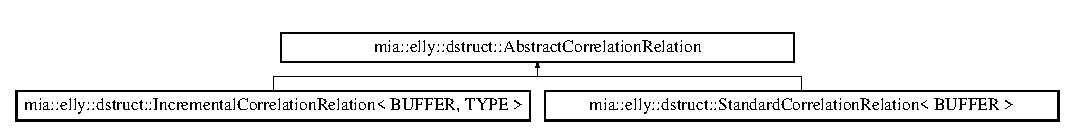
\includegraphics[height=1.359223cm]{classmia_1_1elly_1_1dstruct_1_1_abstract_correlation_relation}
\end{center}
\end{figure}
\subsection*{Public Member Functions}
\begin{DoxyCompactItemize}
\item 
void \hyperlink{classmia_1_1elly_1_1dstruct_1_1_abstract_correlation_relation_a86990596212576f10e6a589fb1eb46b7}{prepare\-\_\-weights} ()
\item 
void \hyperlink{classmia_1_1elly_1_1dstruct_1_1_abstract_correlation_relation_a9d6015d4805d9612d922a1311c2604c3}{dump\-\_\-weights} ()
\item 
void \hyperlink{classmia_1_1elly_1_1dstruct_1_1_abstract_correlation_relation_a3291f1afe2252b5bc97414a96c035505}{lock} (int fid)
\item 
void \hyperlink{classmia_1_1elly_1_1dstruct_1_1_abstract_correlation_relation_a1f81a8c581593c2c5a471687d6369214}{release} (int fid)
\item 
\hyperlink{classmia_1_1elly_1_1dstruct_1_1_abstract_correlation_relation_af6f78017f5af971958660bb946d64171}{$\sim$\-Abstract\-Correlation\-Relation} ()
\item 
\hypertarget{classmia_1_1elly_1_1dstruct_1_1_abstract_correlation_relation_a6fb8ddb076966b2b63be7fbc7b020452}{virtual void $\ast$ {\bfseries lookup} (int fid)=0}\label{classmia_1_1elly_1_1dstruct_1_1_abstract_correlation_relation_a6fb8ddb076966b2b63be7fbc7b020452}

\item 
\hypertarget{classmia_1_1elly_1_1dstruct_1_1_abstract_correlation_relation_a5a783db4f6a78f73a477a80fc51d1c6c}{virtual void {\bfseries prepare} ()=0}\label{classmia_1_1elly_1_1dstruct_1_1_abstract_correlation_relation_a5a783db4f6a78f73a477a80fc51d1c6c}

\item 
\hypertarget{classmia_1_1elly_1_1dstruct_1_1_abstract_correlation_relation_af923ccef57327a22857ade9059863e89}{virtual void {\bfseries update} (int key, void($\ast$func\-\_\-update)(void $\ast$, int, int, int), int vid, int from, int to, bool \hyperlink{classmia_1_1elly_1_1dstruct_1_1_abstract_correlation_relation_a3291f1afe2252b5bc97414a96c035505}{lock})=0}\label{classmia_1_1elly_1_1dstruct_1_1_abstract_correlation_relation_af923ccef57327a22857ade9059863e89}

\end{DoxyCompactItemize}
\subsection*{Public Attributes}
\begin{DoxyCompactItemize}
\item 
\hypertarget{classmia_1_1elly_1_1dstruct_1_1_abstract_correlation_relation_a800bb55573026e2826af0a1326ceb401}{std\-::string {\bfseries factor\-\_\-name}}\label{classmia_1_1elly_1_1dstruct_1_1_abstract_correlation_relation_a800bb55573026e2826af0a1326ceb401}

\item 
int \hyperlink{classmia_1_1elly_1_1dstruct_1_1_abstract_correlation_relation_a3747a084efa5095d4808819bb012ae65}{factor\-\_\-id}
\item 
int \hyperlink{classmia_1_1elly_1_1dstruct_1_1_abstract_correlation_relation_ac7216c599394d0b1026bb4f7a161f6a4}{function\-\_\-id}
\item 
std\-::string \hyperlink{classmia_1_1elly_1_1dstruct_1_1_abstract_correlation_relation_a21e302ad723c9e0c99eb81c5bc420779}{filename}
\item 
std\-::string \hyperlink{classmia_1_1elly_1_1dstruct_1_1_abstract_correlation_relation_ae96b4f7de4d2e53b3a3ea38b14e90838}{filetype}
\item 
std\-::string \hyperlink{classmia_1_1elly_1_1dstruct_1_1_abstract_correlation_relation_a528970ab644de5fa8958bc8b26917664}{mapfilename}
\item 
std\-::vector$<$ double $>$ \hyperlink{classmia_1_1elly_1_1dstruct_1_1_abstract_correlation_relation_a8a094d32441aca190c2ab019407de95a}{weights}
\item 
std\-::vector$<$ pthread\-\_\-mutex\-\_\-t $\ast$ $>$ \hyperlink{classmia_1_1elly_1_1dstruct_1_1_abstract_correlation_relation_a10a0c3ac052768f044f4c0a7da5f2a80}{sems}
\item 
int \hyperlink{classmia_1_1elly_1_1dstruct_1_1_abstract_correlation_relation_a65756a92a296e0e9041b043cee64d8b0}{nfactor}
\end{DoxyCompactItemize}


\subsection{Detailed Description}
Abstract class for unifying \hyperlink{classmia_1_1elly_1_1dstruct_1_1_standard_correlation_relation}{mia\-::elly\-::dstruct\-::\-Standard\-Correlation\-Relation} and \hyperlink{classmia_1_1elly_1_1dstruct_1_1_incremental_correlation_relation}{mia\-::elly\-::dstruct\-::\-Incremental\-Correlation\-Relation}. 

\subsection{Constructor \& Destructor Documentation}
\hypertarget{classmia_1_1elly_1_1dstruct_1_1_abstract_correlation_relation_af6f78017f5af971958660bb946d64171}{\index{mia\-::elly\-::dstruct\-::\-Abstract\-Correlation\-Relation@{mia\-::elly\-::dstruct\-::\-Abstract\-Correlation\-Relation}!$\sim$\-Abstract\-Correlation\-Relation@{$\sim$\-Abstract\-Correlation\-Relation}}
\index{$\sim$\-Abstract\-Correlation\-Relation@{$\sim$\-Abstract\-Correlation\-Relation}!mia::elly::dstruct::AbstractCorrelationRelation@{mia\-::elly\-::dstruct\-::\-Abstract\-Correlation\-Relation}}
\subsubsection[{$\sim$\-Abstract\-Correlation\-Relation}]{\setlength{\rightskip}{0pt plus 5cm}mia\-::elly\-::dstruct\-::\-Abstract\-Correlation\-Relation\-::$\sim$\-Abstract\-Correlation\-Relation (
\begin{DoxyParamCaption}
{}
\end{DoxyParamCaption}
)\hspace{0.3cm}{\ttfamily [inline]}}}\label{classmia_1_1elly_1_1dstruct_1_1_abstract_correlation_relation_af6f78017f5af971958660bb946d64171}
Deconstructor. Release and destroy all locks. 

\subsection{Member Function Documentation}
\hypertarget{classmia_1_1elly_1_1dstruct_1_1_abstract_correlation_relation_a9d6015d4805d9612d922a1311c2604c3}{\index{mia\-::elly\-::dstruct\-::\-Abstract\-Correlation\-Relation@{mia\-::elly\-::dstruct\-::\-Abstract\-Correlation\-Relation}!dump\-\_\-weights@{dump\-\_\-weights}}
\index{dump\-\_\-weights@{dump\-\_\-weights}!mia::elly::dstruct::AbstractCorrelationRelation@{mia\-::elly\-::dstruct\-::\-Abstract\-Correlation\-Relation}}
\subsubsection[{dump\-\_\-weights}]{\setlength{\rightskip}{0pt plus 5cm}void mia\-::elly\-::dstruct\-::\-Abstract\-Correlation\-Relation\-::dump\-\_\-weights (
\begin{DoxyParamCaption}
{}
\end{DoxyParamCaption}
)\hspace{0.3cm}{\ttfamily [inline]}}}\label{classmia_1_1elly_1_1dstruct_1_1_abstract_correlation_relation_a9d6015d4805d9612d922a1311c2604c3}
Refresh weight file by current weights. \hypertarget{classmia_1_1elly_1_1dstruct_1_1_abstract_correlation_relation_a3291f1afe2252b5bc97414a96c035505}{\index{mia\-::elly\-::dstruct\-::\-Abstract\-Correlation\-Relation@{mia\-::elly\-::dstruct\-::\-Abstract\-Correlation\-Relation}!lock@{lock}}
\index{lock@{lock}!mia::elly::dstruct::AbstractCorrelationRelation@{mia\-::elly\-::dstruct\-::\-Abstract\-Correlation\-Relation}}
\subsubsection[{lock}]{\setlength{\rightskip}{0pt plus 5cm}void mia\-::elly\-::dstruct\-::\-Abstract\-Correlation\-Relation\-::lock (
\begin{DoxyParamCaption}
\item[{int}]{fid}
\end{DoxyParamCaption}
)\hspace{0.3cm}{\ttfamily [inline]}}}\label{classmia_1_1elly_1_1dstruct_1_1_abstract_correlation_relation_a3291f1afe2252b5bc97414a96c035505}
Lock a factor. \hypertarget{classmia_1_1elly_1_1dstruct_1_1_abstract_correlation_relation_a86990596212576f10e6a589fb1eb46b7}{\index{mia\-::elly\-::dstruct\-::\-Abstract\-Correlation\-Relation@{mia\-::elly\-::dstruct\-::\-Abstract\-Correlation\-Relation}!prepare\-\_\-weights@{prepare\-\_\-weights}}
\index{prepare\-\_\-weights@{prepare\-\_\-weights}!mia::elly::dstruct::AbstractCorrelationRelation@{mia\-::elly\-::dstruct\-::\-Abstract\-Correlation\-Relation}}
\subsubsection[{prepare\-\_\-weights}]{\setlength{\rightskip}{0pt plus 5cm}void mia\-::elly\-::dstruct\-::\-Abstract\-Correlation\-Relation\-::prepare\-\_\-weights (
\begin{DoxyParamCaption}
{}
\end{DoxyParamCaption}
)\hspace{0.3cm}{\ttfamily [inline]}}}\label{classmia_1_1elly_1_1dstruct_1_1_abstract_correlation_relation_a86990596212576f10e6a589fb1eb46b7}
load weight file. \hypertarget{classmia_1_1elly_1_1dstruct_1_1_abstract_correlation_relation_a1f81a8c581593c2c5a471687d6369214}{\index{mia\-::elly\-::dstruct\-::\-Abstract\-Correlation\-Relation@{mia\-::elly\-::dstruct\-::\-Abstract\-Correlation\-Relation}!release@{release}}
\index{release@{release}!mia::elly::dstruct::AbstractCorrelationRelation@{mia\-::elly\-::dstruct\-::\-Abstract\-Correlation\-Relation}}
\subsubsection[{release}]{\setlength{\rightskip}{0pt plus 5cm}void mia\-::elly\-::dstruct\-::\-Abstract\-Correlation\-Relation\-::release (
\begin{DoxyParamCaption}
\item[{int}]{fid}
\end{DoxyParamCaption}
)\hspace{0.3cm}{\ttfamily [inline]}}}\label{classmia_1_1elly_1_1dstruct_1_1_abstract_correlation_relation_a1f81a8c581593c2c5a471687d6369214}
Release lock of a factor. 

\subsection{Member Data Documentation}
\hypertarget{classmia_1_1elly_1_1dstruct_1_1_abstract_correlation_relation_a3747a084efa5095d4808819bb012ae65}{\index{mia\-::elly\-::dstruct\-::\-Abstract\-Correlation\-Relation@{mia\-::elly\-::dstruct\-::\-Abstract\-Correlation\-Relation}!factor\-\_\-id@{factor\-\_\-id}}
\index{factor\-\_\-id@{factor\-\_\-id}!mia::elly::dstruct::AbstractCorrelationRelation@{mia\-::elly\-::dstruct\-::\-Abstract\-Correlation\-Relation}}
\subsubsection[{factor\-\_\-id}]{\setlength{\rightskip}{0pt plus 5cm}int mia\-::elly\-::dstruct\-::\-Abstract\-Correlation\-Relation\-::factor\-\_\-id}}\label{classmia_1_1elly_1_1dstruct_1_1_abstract_correlation_relation_a3747a084efa5095d4808819bb012ae65}
I\-D of this correlation relation. \hypertarget{classmia_1_1elly_1_1dstruct_1_1_abstract_correlation_relation_a21e302ad723c9e0c99eb81c5bc420779}{\index{mia\-::elly\-::dstruct\-::\-Abstract\-Correlation\-Relation@{mia\-::elly\-::dstruct\-::\-Abstract\-Correlation\-Relation}!filename@{filename}}
\index{filename@{filename}!mia::elly::dstruct::AbstractCorrelationRelation@{mia\-::elly\-::dstruct\-::\-Abstract\-Correlation\-Relation}}
\subsubsection[{filename}]{\setlength{\rightskip}{0pt plus 5cm}std\-::string mia\-::elly\-::dstruct\-::\-Abstract\-Correlation\-Relation\-::filename}}\label{classmia_1_1elly_1_1dstruct_1_1_abstract_correlation_relation_a21e302ad723c9e0c99eb81c5bc420779}
File that contains this correlation relation. \hypertarget{classmia_1_1elly_1_1dstruct_1_1_abstract_correlation_relation_ae96b4f7de4d2e53b3a3ea38b14e90838}{\index{mia\-::elly\-::dstruct\-::\-Abstract\-Correlation\-Relation@{mia\-::elly\-::dstruct\-::\-Abstract\-Correlation\-Relation}!filetype@{filetype}}
\index{filetype@{filetype}!mia::elly::dstruct::AbstractCorrelationRelation@{mia\-::elly\-::dstruct\-::\-Abstract\-Correlation\-Relation}}
\subsubsection[{filetype}]{\setlength{\rightskip}{0pt plus 5cm}std\-::string mia\-::elly\-::dstruct\-::\-Abstract\-Correlation\-Relation\-::filetype}}\label{classmia_1_1elly_1_1dstruct_1_1_abstract_correlation_relation_ae96b4f7de4d2e53b3a3ea38b14e90838}
Type of correlation relation file. \{tsv\} \hypertarget{classmia_1_1elly_1_1dstruct_1_1_abstract_correlation_relation_ac7216c599394d0b1026bb4f7a161f6a4}{\index{mia\-::elly\-::dstruct\-::\-Abstract\-Correlation\-Relation@{mia\-::elly\-::dstruct\-::\-Abstract\-Correlation\-Relation}!function\-\_\-id@{function\-\_\-id}}
\index{function\-\_\-id@{function\-\_\-id}!mia::elly::dstruct::AbstractCorrelationRelation@{mia\-::elly\-::dstruct\-::\-Abstract\-Correlation\-Relation}}
\subsubsection[{function\-\_\-id}]{\setlength{\rightskip}{0pt plus 5cm}int mia\-::elly\-::dstruct\-::\-Abstract\-Correlation\-Relation\-::function\-\_\-id}}\label{classmia_1_1elly_1_1dstruct_1_1_abstract_correlation_relation_ac7216c599394d0b1026bb4f7a161f6a4}
Factor I\-D -- for potential/update/gradient functions. \hypertarget{classmia_1_1elly_1_1dstruct_1_1_abstract_correlation_relation_a528970ab644de5fa8958bc8b26917664}{\index{mia\-::elly\-::dstruct\-::\-Abstract\-Correlation\-Relation@{mia\-::elly\-::dstruct\-::\-Abstract\-Correlation\-Relation}!mapfilename@{mapfilename}}
\index{mapfilename@{mapfilename}!mia::elly::dstruct::AbstractCorrelationRelation@{mia\-::elly\-::dstruct\-::\-Abstract\-Correlation\-Relation}}
\subsubsection[{mapfilename}]{\setlength{\rightskip}{0pt plus 5cm}std\-::string mia\-::elly\-::dstruct\-::\-Abstract\-Correlation\-Relation\-::mapfilename}}\label{classmia_1_1elly_1_1dstruct_1_1_abstract_correlation_relation_a528970ab644de5fa8958bc8b26917664}
File that contains weights. \hypertarget{classmia_1_1elly_1_1dstruct_1_1_abstract_correlation_relation_a65756a92a296e0e9041b043cee64d8b0}{\index{mia\-::elly\-::dstruct\-::\-Abstract\-Correlation\-Relation@{mia\-::elly\-::dstruct\-::\-Abstract\-Correlation\-Relation}!nfactor@{nfactor}}
\index{nfactor@{nfactor}!mia::elly::dstruct::AbstractCorrelationRelation@{mia\-::elly\-::dstruct\-::\-Abstract\-Correlation\-Relation}}
\subsubsection[{nfactor}]{\setlength{\rightskip}{0pt plus 5cm}int mia\-::elly\-::dstruct\-::\-Abstract\-Correlation\-Relation\-::nfactor}}\label{classmia_1_1elly_1_1dstruct_1_1_abstract_correlation_relation_a65756a92a296e0e9041b043cee64d8b0}
Number of factors being loaded. \hypertarget{classmia_1_1elly_1_1dstruct_1_1_abstract_correlation_relation_a10a0c3ac052768f044f4c0a7da5f2a80}{\index{mia\-::elly\-::dstruct\-::\-Abstract\-Correlation\-Relation@{mia\-::elly\-::dstruct\-::\-Abstract\-Correlation\-Relation}!sems@{sems}}
\index{sems@{sems}!mia::elly::dstruct::AbstractCorrelationRelation@{mia\-::elly\-::dstruct\-::\-Abstract\-Correlation\-Relation}}
\subsubsection[{sems}]{\setlength{\rightskip}{0pt plus 5cm}std\-::vector$<$pthread\-\_\-mutex\-\_\-t$\ast$ $>$ mia\-::elly\-::dstruct\-::\-Abstract\-Correlation\-Relation\-::sems}}\label{classmia_1_1elly_1_1dstruct_1_1_abstract_correlation_relation_a10a0c3ac052768f044f4c0a7da5f2a80}
In-\/memory locks for factors in this correlation relation. \hypertarget{classmia_1_1elly_1_1dstruct_1_1_abstract_correlation_relation_a8a094d32441aca190c2ab019407de95a}{\index{mia\-::elly\-::dstruct\-::\-Abstract\-Correlation\-Relation@{mia\-::elly\-::dstruct\-::\-Abstract\-Correlation\-Relation}!weights@{weights}}
\index{weights@{weights}!mia::elly::dstruct::AbstractCorrelationRelation@{mia\-::elly\-::dstruct\-::\-Abstract\-Correlation\-Relation}}
\subsubsection[{weights}]{\setlength{\rightskip}{0pt plus 5cm}std\-::vector$<$double$>$ mia\-::elly\-::dstruct\-::\-Abstract\-Correlation\-Relation\-::weights}}\label{classmia_1_1elly_1_1dstruct_1_1_abstract_correlation_relation_a8a094d32441aca190c2ab019407de95a}
In-\/memory vector that stores weights. 

The documentation for this class was generated from the following file\-:\begin{DoxyCompactItemize}
\item 
/\-Users/czhang/\-Desktop/\-Codes/mia/src/elly/elly/dstruct/Abstract\-Correlation\-Relation.\-h\end{DoxyCompactItemize}

\hypertarget{classmia_1_1sm_1_1_buffer__mm}{\section{mia\-:\-:sm\-:\-:Buffer\-\_\-mm$<$ P\-A\-G\-E, T\-Y\-P\-E $>$ Class Template Reference}
\label{classmia_1_1sm_1_1_buffer__mm}\index{mia\-::sm\-::\-Buffer\-\_\-mm$<$ P\-A\-G\-E, T\-Y\-P\-E $>$@{mia\-::sm\-::\-Buffer\-\_\-mm$<$ P\-A\-G\-E, T\-Y\-P\-E $>$}}
}
\subsection*{Public Member Functions}
\begin{DoxyCompactItemize}
\item 
\hypertarget{classmia_1_1sm_1_1_buffer__mm_a1679c5089078fc73b6aa33b1817cf0ca}{T\-Y\-P\-E {\bfseries get} (int pageid, int slotid)}\label{classmia_1_1sm_1_1_buffer__mm_a1679c5089078fc73b6aa33b1817cf0ca}

\item 
\hypertarget{classmia_1_1sm_1_1_buffer__mm_a23322e755d5d8f61b60fbb97243658ff}{void {\bfseries set} (int pageid, int slotid, T\-Y\-P\-E obj)}\label{classmia_1_1sm_1_1_buffer__mm_a23322e755d5d8f61b60fbb97243658ff}

\item 
\hypertarget{classmia_1_1sm_1_1_buffer__mm_ad4cb43214f27c955b9a9be4903adf951}{void {\bfseries push} (T\-Y\-P\-E obj, int \&pageid, int \&slotid)}\label{classmia_1_1sm_1_1_buffer__mm_ad4cb43214f27c955b9a9be4903adf951}

\end{DoxyCompactItemize}
\subsection*{Public Attributes}
\begin{DoxyCompactItemize}
\item 
\hypertarget{classmia_1_1sm_1_1_buffer__mm_a2cdd9bd381e34e5a27b546133ea0c089}{int {\bfseries cpage}}\label{classmia_1_1sm_1_1_buffer__mm_a2cdd9bd381e34e5a27b546133ea0c089}

\item 
\hypertarget{classmia_1_1sm_1_1_buffer__mm_ac4c2a6a85efca2365dc11d99beb731ff}{int {\bfseries miss\-\_\-read}}\label{classmia_1_1sm_1_1_buffer__mm_ac4c2a6a85efca2365dc11d99beb731ff}

\item 
\hypertarget{classmia_1_1sm_1_1_buffer__mm_a7a095f928a1c8fc6760b793ae40888f3}{int {\bfseries miss\-\_\-write}}\label{classmia_1_1sm_1_1_buffer__mm_a7a095f928a1c8fc6760b793ae40888f3}

\item 
\hypertarget{classmia_1_1sm_1_1_buffer__mm_ab2dac9275c5cea293d4e62e6cb6f5b75}{std\-::vector$<$ P\-A\-G\-E$<$ T\-Y\-P\-E $>$ $>$ {\bfseries pages}}\label{classmia_1_1sm_1_1_buffer__mm_ab2dac9275c5cea293d4e62e6cb6f5b75}

\end{DoxyCompactItemize}


The documentation for this class was generated from the following file\-:\begin{DoxyCompactItemize}
\item 
/\-Users/czhang/\-Desktop/\-Codes/mia/src/storageman\-\_\-old/storageman/Buffer\-\_\-mm.\-h\end{DoxyCompactItemize}

\hypertarget{classmia_1_1sm_1_1_buffer__mmap}{\section{mia\-:\-:sm\-:\-:Buffer\-\_\-mmap$<$ P\-A\-G\-E, T\-Y\-P\-E $>$ Class Template Reference}
\label{classmia_1_1sm_1_1_buffer__mmap}\index{mia\-::sm\-::\-Buffer\-\_\-mmap$<$ P\-A\-G\-E, T\-Y\-P\-E $>$@{mia\-::sm\-::\-Buffer\-\_\-mmap$<$ P\-A\-G\-E, T\-Y\-P\-E $>$}}
}
\subsection*{Public Member Functions}
\begin{DoxyCompactItemize}
\item 
\hypertarget{classmia_1_1sm_1_1_buffer__mmap_a1b5a3c28e2be2b8d28b6f0e83c67eb27}{T\-Y\-P\-E {\bfseries get} (int pageid, int slotid)}\label{classmia_1_1sm_1_1_buffer__mmap_a1b5a3c28e2be2b8d28b6f0e83c67eb27}

\item 
\hypertarget{classmia_1_1sm_1_1_buffer__mmap_afa43a903959215eb074be496d3afc67a}{void {\bfseries set} (int pageid, int slotid, T\-Y\-P\-E obj)}\label{classmia_1_1sm_1_1_buffer__mmap_afa43a903959215eb074be496d3afc67a}

\item 
\hypertarget{classmia_1_1sm_1_1_buffer__mmap_aed36ed7fcf3a9ca9d9300f2caff2ee60}{void {\bfseries push} (T\-Y\-P\-E obj, int \&pageid, int \&slotid)}\label{classmia_1_1sm_1_1_buffer__mmap_aed36ed7fcf3a9ca9d9300f2caff2ee60}

\end{DoxyCompactItemize}
\subsection*{Public Attributes}
\begin{DoxyCompactItemize}
\item 
\hypertarget{classmia_1_1sm_1_1_buffer__mmap_a4426c619759c9d3e9832c7a94b3b90b6}{int {\bfseries cpage}}\label{classmia_1_1sm_1_1_buffer__mmap_a4426c619759c9d3e9832c7a94b3b90b6}

\item 
\hypertarget{classmia_1_1sm_1_1_buffer__mmap_ad9e564fdacc8dece3dd99bb75aabc075}{int {\bfseries miss\-\_\-read}}\label{classmia_1_1sm_1_1_buffer__mmap_ad9e564fdacc8dece3dd99bb75aabc075}

\item 
\hypertarget{classmia_1_1sm_1_1_buffer__mmap_a420fcbd775fe889c4a3cdbdf12543374}{int {\bfseries miss\-\_\-write}}\label{classmia_1_1sm_1_1_buffer__mmap_a420fcbd775fe889c4a3cdbdf12543374}

\item 
\hypertarget{classmia_1_1sm_1_1_buffer__mmap_aec47baf6260d505617de2d405a97a788}{int {\bfseries fd}}\label{classmia_1_1sm_1_1_buffer__mmap_aec47baf6260d505617de2d405a97a788}

\item 
\hypertarget{classmia_1_1sm_1_1_buffer__mmap_ab49e61b9044b8c91f4cc393d70311652}{P\-A\-G\-E$<$ T\-Y\-P\-E $>$ $\ast$ {\bfseries pages}}\label{classmia_1_1sm_1_1_buffer__mmap_ab49e61b9044b8c91f4cc393d70311652}

\item 
\hypertarget{classmia_1_1sm_1_1_buffer__mmap_a1208ae10b48ad3d5746787bd1d34a424}{int {\bfseries cnpages}}\label{classmia_1_1sm_1_1_buffer__mmap_a1208ae10b48ad3d5746787bd1d34a424}

\end{DoxyCompactItemize}


The documentation for this class was generated from the following file\-:\begin{DoxyCompactItemize}
\item 
storageman/storageman/Buffer\-\_\-mmap.\-h\end{DoxyCompactItemize}

\hypertarget{classmia_1_1elly_1_1utils_1_1_config}{\section{mia\-:\-:elly\-:\-:utils\-:\-:Config Class Reference}
\label{classmia_1_1elly_1_1utils_1_1_config}\index{mia\-::elly\-::utils\-::\-Config@{mia\-::elly\-::utils\-::\-Config}}
}


{\ttfamily \#include $<$Config.\-h$>$}

\subsection*{Public Attributes}
\begin{DoxyCompactItemize}
\item 
\hypertarget{classmia_1_1elly_1_1utils_1_1_config_a39bcb2abda96acaf66b1c176e6ce63cb}{std\-::string {\bfseries version\-\_\-number}}\label{classmia_1_1elly_1_1utils_1_1_config_a39bcb2abda96acaf66b1c176e6ce63cb}

\item 
\hypertarget{classmia_1_1elly_1_1utils_1_1_config_a2c0b3e7d0478530afb5e031647f4d6ca}{std\-::string {\bfseries ui\-\_\-verbose}}\label{classmia_1_1elly_1_1utils_1_1_config_a2c0b3e7d0478530afb5e031647f4d6ca}

\item 
\hypertarget{classmia_1_1elly_1_1utils_1_1_config_a6a6fd92e60395b6cf875ed8a6782e29b}{std\-::string {\bfseries ui\-\_\-logfile}}\label{classmia_1_1elly_1_1utils_1_1_config_a6a6fd92e60395b6cf875ed8a6782e29b}

\item 
\hypertarget{classmia_1_1elly_1_1utils_1_1_config_aa6cf2371478ffbe27d74a489f102d006}{std\-::string {\bfseries ui\-\_\-logverbose}}\label{classmia_1_1elly_1_1utils_1_1_config_aa6cf2371478ffbe27d74a489f102d006}

\item 
\hypertarget{classmia_1_1elly_1_1utils_1_1_config_a6e0dd458d30629613b2fe131a1aca048}{std\-::string {\bfseries rt\-\_\-input}}\label{classmia_1_1elly_1_1utils_1_1_config_a6e0dd458d30629613b2fe131a1aca048}

\item 
\hypertarget{classmia_1_1elly_1_1utils_1_1_config_abab18c0b0e4819432851e764ee8b0091}{std\-::string {\bfseries rt\-\_\-output}}\label{classmia_1_1elly_1_1utils_1_1_config_abab18c0b0e4819432851e764ee8b0091}

\item 
\hypertarget{classmia_1_1elly_1_1utils_1_1_config_a4b826188e5713ed198ce32a43df0c784}{std\-::string {\bfseries rt\-\_\-workdir}}\label{classmia_1_1elly_1_1utils_1_1_config_a4b826188e5713ed198ce32a43df0c784}

\item 
\hypertarget{classmia_1_1elly_1_1utils_1_1_config_a707f5507b5edffd77ddf11df475b95be}{std\-::string {\bfseries rt\-\_\-mode}}\label{classmia_1_1elly_1_1utils_1_1_config_a707f5507b5edffd77ddf11df475b95be}

\item 
\hypertarget{classmia_1_1elly_1_1utils_1_1_config_a187f5440b50ae628956ff488b7454be3}{int {\bfseries rt\-\_\-thin}}\label{classmia_1_1elly_1_1utils_1_1_config_a187f5440b50ae628956ff488b7454be3}

\item 
\hypertarget{classmia_1_1elly_1_1utils_1_1_config_a3b9428eb85f41e6aa87f0f3cefd50768}{int {\bfseries rt\-\_\-burnin}}\label{classmia_1_1elly_1_1utils_1_1_config_a3b9428eb85f41e6aa87f0f3cefd50768}

\item 
\hypertarget{classmia_1_1elly_1_1utils_1_1_config_aaa8c9afd38e09a083e64a7e7c419c11e}{int {\bfseries rt\-\_\-nepoch}}\label{classmia_1_1elly_1_1utils_1_1_config_aaa8c9afd38e09a083e64a7e7c419c11e}

\item 
\hypertarget{classmia_1_1elly_1_1utils_1_1_config_a65dbf0244ef85dc3133d647a6d8dd80a}{double {\bfseries rt\-\_\-learn\-\_\-initstep}}\label{classmia_1_1elly_1_1utils_1_1_config_a65dbf0244ef85dc3133d647a6d8dd80a}

\item 
\hypertarget{classmia_1_1elly_1_1utils_1_1_config_a0d91550f153a44d7d1470527e72a8441}{double {\bfseries rt\-\_\-learn\-\_\-decay}}\label{classmia_1_1elly_1_1utils_1_1_config_a0d91550f153a44d7d1470527e72a8441}

\item 
\hypertarget{classmia_1_1elly_1_1utils_1_1_config_ae62d69a897e21e266db896580e4fd5ef}{bool {\bfseries rt\-\_\-lock}}\label{classmia_1_1elly_1_1utils_1_1_config_ae62d69a897e21e266db896580e4fd5ef}

\item 
\hypertarget{classmia_1_1elly_1_1utils_1_1_config_a7bd840f563c4bed96e34cdcb5c1eba2d}{bool {\bfseries rt\-\_\-is\-\_\-log\-\_\-system}}\label{classmia_1_1elly_1_1utils_1_1_config_a7bd840f563c4bed96e34cdcb5c1eba2d}

\item 
\hypertarget{classmia_1_1elly_1_1utils_1_1_config_ad861f616e2e3ab0783dd63ec97d8e760}{int {\bfseries sys\-\_\-nthreads}}\label{classmia_1_1elly_1_1utils_1_1_config_ad861f616e2e3ab0783dd63ec97d8e760}

\item 
\hypertarget{classmia_1_1elly_1_1utils_1_1_config_ac252f6434061ccf1d01e3ea96c13a91b}{bool {\bfseries io\-\_\-ismln}}\label{classmia_1_1elly_1_1utils_1_1_config_ac252f6434061ccf1d01e3ea96c13a91b}

\item 
\hypertarget{classmia_1_1elly_1_1utils_1_1_config_a1e35f73505f5a384536c8c21bdcbca8a}{std\-::string {\bfseries io\-\_\-mln}}\label{classmia_1_1elly_1_1utils_1_1_config_a1e35f73505f5a384536c8c21bdcbca8a}

\end{DoxyCompactItemize}


\subsection{Detailed Description}
Configurations to run elly. \begin{DoxySeeAlso}{See also}
mia\-::elly\-::utils\-::\-Option\-Parser. 
\end{DoxySeeAlso}


The documentation for this class was generated from the following file\-:\begin{DoxyCompactItemize}
\item 
elly/elly/utils/Config.\-h\end{DoxyCompactItemize}

\hypertarget{classmia_1_1elly_1_1_elly}{\section{mia\-:\-:elly\-:\-:Elly Class Reference}
\label{classmia_1_1elly_1_1_elly}\index{mia\-::elly\-::\-Elly@{mia\-::elly\-::\-Elly}}
}
\subsection*{Public Member Functions}
\begin{DoxyCompactItemize}
\item 
\hypertarget{classmia_1_1elly_1_1_elly_a3b7f9dad7a69a8c6f6063a4568df69af}{void {\bfseries generate\-\_\-tasks\-\_\-and\-\_\-map} (\hyperlink{classmia_1_1elly_1_1mat_1_1_materialization__lazy}{mia\-::elly\-::mat\-::\-Materialization\-\_\-lazy} $\ast$mat, double temparature=-\/1, bool tally=false, bool train=false, double step\-Size=-\/1)}\label{classmia_1_1elly_1_1_elly_a3b7f9dad7a69a8c6f6063a4568df69af}

\item 
\hypertarget{classmia_1_1elly_1_1_elly_a6a66d52e4d4c84aee9360b12bacb8182}{{\bfseries Elly} (\hyperlink{classmia_1_1elly_1_1utils_1_1_config}{mia\-::elly\-::utils\-::\-Config} $\ast$\-\_\-config)}\label{classmia_1_1elly_1_1_elly_a6a66d52e4d4c84aee9360b12bacb8182}

\item 
\hypertarget{classmia_1_1elly_1_1_elly_aae3ca29aa589d10b32e8680725b8bcbc}{void {\bfseries map} ()}\label{classmia_1_1elly_1_1_elly_aae3ca29aa589d10b32e8680725b8bcbc}

\item 
\hypertarget{classmia_1_1elly_1_1_elly_aac1929f8be3fdafd7cc248877fb8c11c}{double {\bfseries sa\-\_\-temparature} (int \-\_\-nepoch)}\label{classmia_1_1elly_1_1_elly_aac1929f8be3fdafd7cc248877fb8c11c}

\item 
\hypertarget{classmia_1_1elly_1_1_elly_aa4da10a8b2e063f632da73f369dcf508}{void {\bfseries run} ()}\label{classmia_1_1elly_1_1_elly_aa4da10a8b2e063f632da73f369dcf508}

\end{DoxyCompactItemize}
\subsection*{Public Attributes}
\begin{DoxyCompactItemize}
\item 
\hypertarget{classmia_1_1elly_1_1_elly_a10d33c83a306c678d2f97afec4a7565e}{int {\bfseries nepoch}}\label{classmia_1_1elly_1_1_elly_a10d33c83a306c678d2f97afec4a7565e}

\item 
\hypertarget{classmia_1_1elly_1_1_elly_a70d6c80bb20a710991443696e53b6570}{std\-::vector$<$ double $>$ $\ast$ {\bfseries vector\-\_\-pool}}\label{classmia_1_1elly_1_1_elly_a70d6c80bb20a710991443696e53b6570}

\item 
\hypertarget{classmia_1_1elly_1_1_elly_a47a74ba9f8cd11ef0cf7e0aba883e6d2}{\hyperlink{classmia_1_1elly_1_1utils_1_1_config}{mia\-::elly\-::utils\-::\-Config} $\ast$ {\bfseries config}}\label{classmia_1_1elly_1_1_elly_a47a74ba9f8cd11ef0cf7e0aba883e6d2}

\end{DoxyCompactItemize}


The documentation for this class was generated from the following file\-:\begin{DoxyCompactItemize}
\item 
elly/elly/main.\-cpp\end{DoxyCompactItemize}

\hypertarget{classfactor__ldacount50}{\section{factor\-\_\-ldacount50 Class Reference}
\label{classfactor__ldacount50}\index{factor\-\_\-ldacount50@{factor\-\_\-ldacount50}}
}


factor class for L\-D\-A ($<$50 topics)  




{\ttfamily \#include $<$factor\-\_\-inits.\-h$>$}

\subsection*{Public Member Functions}
\begin{DoxyCompactItemize}
\item 
\hypertarget{classfactor__ldacount50_a852c648d68d6067e18bfece3af25f30c}{void {\bfseries init\-\_\-aux2} (int aux2)}\label{classfactor__ldacount50_a852c648d68d6067e18bfece3af25f30c}

\item 
\hypertarget{classfactor__ldacount50_a8d028cf2625f639fd07997a9461e231d}{void {\bfseries init\-\_\-aux} (int aux)}\label{classfactor__ldacount50_a8d028cf2625f639fd07997a9461e231d}

\item 
\hypertarget{classfactor__ldacount50_aa53bf93ed30196edaa617624495c509d}{void {\bfseries init} (int vid)}\label{classfactor__ldacount50_aa53bf93ed30196edaa617624495c509d}

\end{DoxyCompactItemize}
\subsection*{Public Attributes}
\begin{DoxyCompactItemize}
\item 
\hypertarget{classfactor__ldacount50_aace3b3d0a4697ebb3baf4479fb5840f8}{int {\bfseries counts} \mbox{[}50\mbox{]}}\label{classfactor__ldacount50_aace3b3d0a4697ebb3baf4479fb5840f8}

\end{DoxyCompactItemize}


\subsection{Detailed Description}
factor class for L\-D\-A ($<$50 topics) 

The documentation for this class was generated from the following file\-:\begin{DoxyCompactItemize}
\item 
/\-Users/czhang/\-Desktop/\-Codes/mia/src/elly/elly/factors/factor\-\_\-inits.\-h\end{DoxyCompactItemize}

\hypertarget{classfactor__vidblock__unigram}{\section{factor\-\_\-vidblock\-\_\-unigram Class Reference}
\label{classfactor__vidblock__unigram}\index{factor\-\_\-vidblock\-\_\-unigram@{factor\-\_\-vidblock\-\_\-unigram}}
}


factor class for general factor relies on V\-I\-Ds.  




{\ttfamily \#include $<$factor\-\_\-inits.\-h$>$}

\subsection*{Public Member Functions}
\begin{DoxyCompactItemize}
\item 
\hypertarget{classfactor__vidblock__unigram_ae3e9a7998e669a52fd00410e17e87648}{void {\bfseries init\-\_\-aux} (int aux)}\label{classfactor__vidblock__unigram_ae3e9a7998e669a52fd00410e17e87648}

\item 
\hypertarget{classfactor__vidblock__unigram_a076f9e660a6cee29835e428db0f9018e}{void {\bfseries init\-\_\-aux2} (int aux2)}\label{classfactor__vidblock__unigram_a076f9e660a6cee29835e428db0f9018e}

\item 
\hypertarget{classfactor__vidblock__unigram_ae47699589594143684c2e82a0f684fac}{void {\bfseries init} (int vid)}\label{classfactor__vidblock__unigram_ae47699589594143684c2e82a0f684fac}

\end{DoxyCompactItemize}
\subsection*{Public Attributes}
\begin{DoxyCompactItemize}
\item 
\hypertarget{classfactor__vidblock__unigram_a1cb8fe295f7b909b339928272315bea8}{\hyperlink{classmia_1_1sm_1_1_ints_block}{mia\-::sm\-::\-Ints\-Block} {\bfseries state}}\label{classfactor__vidblock__unigram_a1cb8fe295f7b909b339928272315bea8}

\end{DoxyCompactItemize}


\subsection{Detailed Description}
factor class for general factor relies on V\-I\-Ds. 

The documentation for this class was generated from the following file\-:\begin{DoxyCompactItemize}
\item 
/\-Users/czhang/\-Desktop/\-Codes/mia/src/elly/elly/factors/factor\-\_\-inits.\-h\end{DoxyCompactItemize}

\hypertarget{classmia_1_1elly_1_1utils_1_1_factor_file_parser}{\section{mia\-:\-:elly\-:\-:utils\-:\-:Factor\-File\-Parser Class Reference}
\label{classmia_1_1elly_1_1utils_1_1_factor_file_parser}\index{mia\-::elly\-::utils\-::\-Factor\-File\-Parser@{mia\-::elly\-::utils\-::\-Factor\-File\-Parser}}
}


Class that contains a set of relations and load them.  




{\ttfamily \#include $<$Factor\-File\-Parser.\-h$>$}

\subsection*{Public Member Functions}
\begin{DoxyCompactItemize}
\item 
\hypertarget{classmia_1_1elly_1_1utils_1_1_factor_file_parser_a96a66a45bba45334c0e6c27f6f37a014}{{\bfseries Factor\-File\-Parser} (std\-::string \-\_\-folder\-\_\-name, \hyperlink{classmia_1_1elly_1_1utils_1_1_config}{elly\-::utils\-::\-Config} $\ast$\-\_\-config)}\label{classmia_1_1elly_1_1utils_1_1_factor_file_parser_a96a66a45bba45334c0e6c27f6f37a014}

\item 
\hypertarget{classmia_1_1elly_1_1utils_1_1_factor_file_parser_a7e4ab3e5026f1daa511bf4eb813200da}{void {\bfseries parse} ()}\label{classmia_1_1elly_1_1utils_1_1_factor_file_parser_a7e4ab3e5026f1daa511bf4eb813200da}

\end{DoxyCompactItemize}
\subsection*{Public Attributes}
\begin{DoxyCompactItemize}
\item 
\hypertarget{classmia_1_1elly_1_1utils_1_1_factor_file_parser_a39e0a9d37ac7f53d3dec871b89cdd0b7}{std\-::string {\bfseries folder\-\_\-name}}\label{classmia_1_1elly_1_1utils_1_1_factor_file_parser_a39e0a9d37ac7f53d3dec871b89cdd0b7}

\item 
\hypertarget{classmia_1_1elly_1_1utils_1_1_factor_file_parser_a5dc9d676ae311be40f4092a083618919}{std\-::string {\bfseries catelog}}\label{classmia_1_1elly_1_1utils_1_1_factor_file_parser_a5dc9d676ae311be40f4092a083618919}

\item 
\hypertarget{classmia_1_1elly_1_1utils_1_1_factor_file_parser_a69922c1caf4cd9cc461f92e6e3df5e31}{\hyperlink{classmia_1_1elly_1_1utils_1_1_config}{elly\-::utils\-::\-Config} $\ast$ {\bfseries config}}\label{classmia_1_1elly_1_1utils_1_1_factor_file_parser_a69922c1caf4cd9cc461f92e6e3df5e31}

\item 
\hypertarget{classmia_1_1elly_1_1utils_1_1_factor_file_parser_acecc638c25c78ef6b94b34347439b37c}{std\-::vector\\*
$<$ \hyperlink{classmia_1_1elly_1_1dstruct_1_1_abstract_correlation_relation}{mia\-::elly\-::dstruct\-::\-Abstract\-Correlation\-Relation} $\ast$ $>$ {\bfseries crs}}\label{classmia_1_1elly_1_1utils_1_1_factor_file_parser_acecc638c25c78ef6b94b34347439b37c}

\item 
\hypertarget{classmia_1_1elly_1_1utils_1_1_factor_file_parser_ac40c1abf8d8de047aa89d83c2fb2bf9d}{\hyperlink{classmia_1_1elly_1_1dstruct_1_1_variable_factor_relation}{mia\-::elly\-::dstruct\-::\-Variable\-Factor\-Relation} {\bfseries vf}}\label{classmia_1_1elly_1_1utils_1_1_factor_file_parser_ac40c1abf8d8de047aa89d83c2fb2bf9d}

\item 
\hypertarget{classmia_1_1elly_1_1utils_1_1_factor_file_parser_ae92501856f9edeffd318af50c778c72b}{\hyperlink{classmia_1_1elly_1_1dstruct_1_1_variable_assignment_relation}{mia\-::elly\-::dstruct\-::\-Variable\-Assignment\-Relation} {\bfseries va}}\label{classmia_1_1elly_1_1utils_1_1_factor_file_parser_ae92501856f9edeffd318af50c778c72b}

\item 
\hypertarget{classmia_1_1elly_1_1utils_1_1_factor_file_parser_a6b0fe25be1e5144f853cd86da9876ecf}{\hyperlink{classmia_1_1elly_1_1dstruct_1_1_variable_tally_relation}{mia\-::elly\-::dstruct\-::\-Variable\-Tally\-Relation} {\bfseries vt}}\label{classmia_1_1elly_1_1utils_1_1_factor_file_parser_a6b0fe25be1e5144f853cd86da9876ecf}

\item 
\hypertarget{classmia_1_1elly_1_1utils_1_1_factor_file_parser_a0e81f19fe8c5c0532273f12b4028b769}{\hyperlink{classmia_1_1elly_1_1dstruct_1_1_variable_training_relation}{mia\-::elly\-::dstruct\-::\-Variable\-Training\-Relation} {\bfseries vtrain}}\label{classmia_1_1elly_1_1utils_1_1_factor_file_parser_a0e81f19fe8c5c0532273f12b4028b769}

\end{DoxyCompactItemize}


\subsection{Detailed Description}
Class that contains a set of relations and load them. 

The documentation for this class was generated from the following file\-:\begin{DoxyCompactItemize}
\item 
/\-Users/czhang/\-Desktop/\-Codes/mia/src/elly/elly/utils/Factor\-File\-Parser.\-h\end{DoxyCompactItemize}

\hypertarget{structmia_1_1elly_1_1utils_1_1_factor_tuple}{\section{mia\-:\-:elly\-:\-:utils\-:\-:Factor\-Tuple Struct Reference}
\label{structmia_1_1elly_1_1utils_1_1_factor_tuple}\index{mia\-::elly\-::utils\-::\-Factor\-Tuple@{mia\-::elly\-::utils\-::\-Factor\-Tuple}}
}
\subsection*{Public Attributes}
\begin{DoxyCompactItemize}
\item 
\hypertarget{structmia_1_1elly_1_1utils_1_1_factor_tuple_a6ac34976c6a9f09302811418be276918}{int {\bfseries factor\-\_\-id}}\label{structmia_1_1elly_1_1utils_1_1_factor_tuple_a6ac34976c6a9f09302811418be276918}

\item 
\hypertarget{structmia_1_1elly_1_1utils_1_1_factor_tuple_a9508c76cec185c05d436cbc92e473155}{int {\bfseries variable\-\_\-id}}\label{structmia_1_1elly_1_1utils_1_1_factor_tuple_a9508c76cec185c05d436cbc92e473155}

\item 
\hypertarget{structmia_1_1elly_1_1utils_1_1_factor_tuple_a5f6a90de690c411850aee354c15776c7}{int {\bfseries pos}}\label{structmia_1_1elly_1_1utils_1_1_factor_tuple_a5f6a90de690c411850aee354c15776c7}

\item 
\hypertarget{structmia_1_1elly_1_1utils_1_1_factor_tuple_a3e51d19b5826a516c691a15be89cec5a}{int {\bfseries aux}}\label{structmia_1_1elly_1_1utils_1_1_factor_tuple_a3e51d19b5826a516c691a15be89cec5a}

\end{DoxyCompactItemize}


The documentation for this struct was generated from the following file\-:\begin{DoxyCompactItemize}
\item 
elly/elly/utils/Common.\-h\end{DoxyCompactItemize}

\hypertarget{classmia_1_1elly_1_1dstruct_1_1_incremental_correlation_relation}{\section{mia\-:\-:elly\-:\-:dstruct\-:\-:Incremental\-Correlation\-Relation$<$ B\-U\-F\-F\-E\-R, T\-Y\-P\-E $>$ Class Template Reference}
\label{classmia_1_1elly_1_1dstruct_1_1_incremental_correlation_relation}\index{mia\-::elly\-::dstruct\-::\-Incremental\-Correlation\-Relation$<$ B\-U\-F\-F\-E\-R, T\-Y\-P\-E $>$@{mia\-::elly\-::dstruct\-::\-Incremental\-Correlation\-Relation$<$ B\-U\-F\-F\-E\-R, T\-Y\-P\-E $>$}}
}


{\ttfamily \#include $<$Incremental\-Correlation\-Relation.\-h$>$}

Inheritance diagram for mia\-:\-:elly\-:\-:dstruct\-:\-:Incremental\-Correlation\-Relation$<$ B\-U\-F\-F\-E\-R, T\-Y\-P\-E $>$\-:\begin{figure}[H]
\begin{center}
\leavevmode
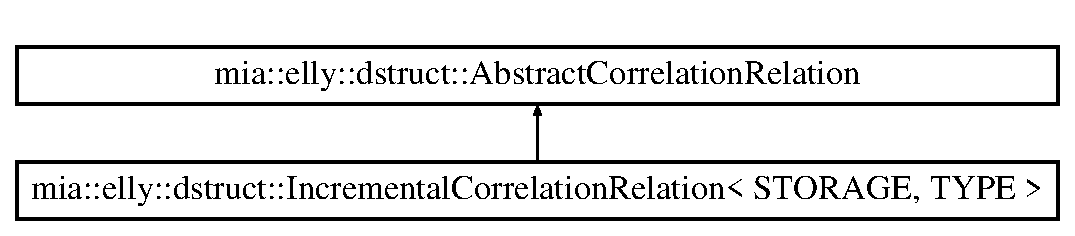
\includegraphics[height=2.000000cm]{classmia_1_1elly_1_1dstruct_1_1_incremental_correlation_relation}
\end{center}
\end{figure}
\subsection*{Public Member Functions}
\begin{DoxyCompactItemize}
\item 
void $\ast$ \hyperlink{classmia_1_1elly_1_1dstruct_1_1_incremental_correlation_relation_a64aa2490a44eb7bebf9accbeb9a04ab4}{lookup} (int fid)
\item 
void \hyperlink{classmia_1_1elly_1_1dstruct_1_1_incremental_correlation_relation_ac8e0e2c5f6650b12c157c3556cebcfc3}{update} (int fid, void($\ast$func\-\_\-update)(void $\ast$, int, int, int), int vid, int from, int to, bool \-\_\-lock)
\item 
\hypertarget{classmia_1_1elly_1_1dstruct_1_1_incremental_correlation_relation_a539746c25aac5cb61de67f6ab08ddcd6}{void {\bfseries prepare} ()}\label{classmia_1_1elly_1_1dstruct_1_1_incremental_correlation_relation_a539746c25aac5cb61de67f6ab08ddcd6}

\end{DoxyCompactItemize}
\subsection*{Public Attributes}
\begin{DoxyCompactItemize}
\item 
\hyperlink{classmia_1_1sm_1_1_key_value__fl__fastmm}{mia\-::sm\-::\-Key\-Value\-\_\-fl\-\_\-fastmm}$<$ T\-Y\-P\-E $>$ \hyperlink{classmia_1_1elly_1_1dstruct_1_1_incremental_correlation_relation_a1fc214b8ab12ac13196aaedd6f629ee2}{kv}
\end{DoxyCompactItemize}


\subsection{Detailed Description}
\subsubsection*{template$<$template$<$ template$<$ class C $>$ class A, class B $>$ class B\-U\-F\-F\-E\-R, class T\-Y\-P\-E$>$class mia\-::elly\-::dstruct\-::\-Incremental\-Correlation\-Relation$<$ B\-U\-F\-F\-E\-R, T\-Y\-P\-E $>$}

Correlation relation in which each factor contains a fixed-\/size state.


\begin{DoxyTemplParams}{Template Parameters}
{\em B\-U\-F\-F\-E\-R} & Buffer to use for this correlation relation. \\
\hline
\end{DoxyTemplParams}


\subsection{Member Function Documentation}
\hypertarget{classmia_1_1elly_1_1dstruct_1_1_incremental_correlation_relation_a64aa2490a44eb7bebf9accbeb9a04ab4}{\index{mia\-::elly\-::dstruct\-::\-Incremental\-Correlation\-Relation@{mia\-::elly\-::dstruct\-::\-Incremental\-Correlation\-Relation}!lookup@{lookup}}
\index{lookup@{lookup}!mia::elly::dstruct::IncrementalCorrelationRelation@{mia\-::elly\-::dstruct\-::\-Incremental\-Correlation\-Relation}}
\subsubsection[{lookup}]{\setlength{\rightskip}{0pt plus 5cm}template$<$template$<$ template$<$ class C $>$ class A, class B $>$ class B\-U\-F\-F\-E\-R, class T\-Y\-P\-E$>$ void$\ast$ {\bf mia\-::elly\-::dstruct\-::\-Incremental\-Correlation\-Relation}$<$ B\-U\-F\-F\-E\-R, T\-Y\-P\-E $>$\-::lookup (
\begin{DoxyParamCaption}
\item[{int}]{fid}
\end{DoxyParamCaption}
)\hspace{0.3cm}{\ttfamily [inline]}, {\ttfamily [virtual]}}}\label{classmia_1_1elly_1_1dstruct_1_1_incremental_correlation_relation_a64aa2490a44eb7bebf9accbeb9a04ab4}
given a factor I\-D, return the pointer to its state. 

Implements \hyperlink{classmia_1_1elly_1_1dstruct_1_1_abstract_correlation_relation}{mia\-::elly\-::dstruct\-::\-Abstract\-Correlation\-Relation}.

\hypertarget{classmia_1_1elly_1_1dstruct_1_1_incremental_correlation_relation_ac8e0e2c5f6650b12c157c3556cebcfc3}{\index{mia\-::elly\-::dstruct\-::\-Incremental\-Correlation\-Relation@{mia\-::elly\-::dstruct\-::\-Incremental\-Correlation\-Relation}!update@{update}}
\index{update@{update}!mia::elly::dstruct::IncrementalCorrelationRelation@{mia\-::elly\-::dstruct\-::\-Incremental\-Correlation\-Relation}}
\subsubsection[{update}]{\setlength{\rightskip}{0pt plus 5cm}template$<$template$<$ template$<$ class C $>$ class A, class B $>$ class B\-U\-F\-F\-E\-R, class T\-Y\-P\-E$>$ void {\bf mia\-::elly\-::dstruct\-::\-Incremental\-Correlation\-Relation}$<$ B\-U\-F\-F\-E\-R, T\-Y\-P\-E $>$\-::update (
\begin{DoxyParamCaption}
\item[{int}]{fid, }
\item[{void($\ast$)(void $\ast$, int, int, int)}]{func\-\_\-update, }
\item[{int}]{vid, }
\item[{int}]{from, }
\item[{int}]{to, }
\item[{bool}]{\-\_\-lock}
\end{DoxyParamCaption}
)\hspace{0.3cm}{\ttfamily [inline]}, {\ttfamily [virtual]}}}\label{classmia_1_1elly_1_1dstruct_1_1_incremental_correlation_relation_ac8e0e2c5f6650b12c157c3556cebcfc3}
Update the state given new assignment of variables.


\begin{DoxyParams}{Parameters}
{\em fid} & factor I\-D \\
\hline
{\em func\-\_\-update} & function pointer to update function \\
\hline
{\em vid} & variable I\-D to be updated \\
\hline
{\em } & \\
\hline
\end{DoxyParams}


Implements \hyperlink{classmia_1_1elly_1_1dstruct_1_1_abstract_correlation_relation}{mia\-::elly\-::dstruct\-::\-Abstract\-Correlation\-Relation}.



\subsection{Member Data Documentation}
\hypertarget{classmia_1_1elly_1_1dstruct_1_1_incremental_correlation_relation_a1fc214b8ab12ac13196aaedd6f629ee2}{\index{mia\-::elly\-::dstruct\-::\-Incremental\-Correlation\-Relation@{mia\-::elly\-::dstruct\-::\-Incremental\-Correlation\-Relation}!kv@{kv}}
\index{kv@{kv}!mia::elly::dstruct::IncrementalCorrelationRelation@{mia\-::elly\-::dstruct\-::\-Incremental\-Correlation\-Relation}}
\subsubsection[{kv}]{\setlength{\rightskip}{0pt plus 5cm}template$<$template$<$ template$<$ class C $>$ class A, class B $>$ class B\-U\-F\-F\-E\-R, class T\-Y\-P\-E$>$ {\bf mia\-::sm\-::\-Key\-Value\-\_\-fl\-\_\-fastmm}$<$T\-Y\-P\-E$>$ {\bf mia\-::elly\-::dstruct\-::\-Incremental\-Correlation\-Relation}$<$ B\-U\-F\-F\-E\-R, T\-Y\-P\-E $>$\-::kv}}\label{classmia_1_1elly_1_1dstruct_1_1_incremental_correlation_relation_a1fc214b8ab12ac13196aaedd6f629ee2}
In-\/memory key value store that maps factor I\-D to its state. 

The documentation for this class was generated from the following file\-:\begin{DoxyCompactItemize}
\item 
elly/elly/dstruct/Incremental\-Correlation\-Relation.\-h\end{DoxyCompactItemize}

\hypertarget{classmia_1_1sm_1_1_int_pair}{\section{mia\-:\-:sm\-:\-:Int\-Pair Class Reference}
\label{classmia_1_1sm_1_1_int_pair}\index{mia\-::sm\-::\-Int\-Pair@{mia\-::sm\-::\-Int\-Pair}}
}
\subsection*{Public Attributes}
\begin{DoxyCompactItemize}
\item 
\hypertarget{classmia_1_1sm_1_1_int_pair_a6b26fd35105cf8003c149fc7bb291d77}{int {\bfseries first}}\label{classmia_1_1sm_1_1_int_pair_a6b26fd35105cf8003c149fc7bb291d77}

\item 
\hypertarget{classmia_1_1sm_1_1_int_pair_ac7ddf6cbe2480340524e6c7264be4253}{int {\bfseries second}}\label{classmia_1_1sm_1_1_int_pair_ac7ddf6cbe2480340524e6c7264be4253}

\end{DoxyCompactItemize}


The documentation for this class was generated from the following file\-:\begin{DoxyCompactItemize}
\item 
storageman/storageman/Ints\-Block.\-h\end{DoxyCompactItemize}

\hypertarget{classmia_1_1sm_1_1_ints_block}{\section{mia\-:\-:sm\-:\-:Ints\-Block Class Reference}
\label{classmia_1_1sm_1_1_ints_block}\index{mia\-::sm\-::\-Ints\-Block@{mia\-::sm\-::\-Ints\-Block}}
}
\subsection*{Public Member Functions}
\begin{DoxyCompactItemize}
\item 
\hypertarget{classmia_1_1sm_1_1_ints_block_a5d9e15e2d7196a84746cbbb2db2b90aa}{{\footnotesize template$<$class T\-Y\-P\-E $>$ }\\void {\bfseries append} (T\-Y\-P\-E obj)}\label{classmia_1_1sm_1_1_ints_block_a5d9e15e2d7196a84746cbbb2db2b90aa}

\item 
\hypertarget{classmia_1_1sm_1_1_ints_block_a2f8109be82fff2222b1163e4ea82e223}{{\footnotesize template$<$class T\-Y\-P\-E $>$ }\\T\-Y\-P\-E {\bfseries get} (int nint)}\label{classmia_1_1sm_1_1_ints_block_a2f8109be82fff2222b1163e4ea82e223}

\end{DoxyCompactItemize}
\subsection*{Public Attributes}
\begin{DoxyCompactItemize}
\item 
\hypertarget{classmia_1_1sm_1_1_ints_block_a0081a01b017e835aaa428875a6428409}{int {\bfseries size}}\label{classmia_1_1sm_1_1_ints_block_a0081a01b017e835aaa428875a6428409}

\item 
\hypertarget{classmia_1_1sm_1_1_ints_block_a5bca4c9ccc401e60a045233adaef3d8f}{int {\bfseries content} \mbox{[}Mem\-Block\-N\-I\-N\-T\mbox{]}}\label{classmia_1_1sm_1_1_ints_block_a5bca4c9ccc401e60a045233adaef3d8f}

\end{DoxyCompactItemize}


The documentation for this class was generated from the following file\-:\begin{DoxyCompactItemize}
\item 
storageman/storageman/Ints\-Block.\-h\end{DoxyCompactItemize}

\hypertarget{classmia_1_1sm_1_1_key_value__fl}{\section{mia\-:\-:sm\-:\-:Key\-Value\-\_\-fl$<$ B\-U\-F\-F\-E\-R, T\-Y\-P\-E $>$ Class Template Reference}
\label{classmia_1_1sm_1_1_key_value__fl}\index{mia\-::sm\-::\-Key\-Value\-\_\-fl$<$ B\-U\-F\-F\-E\-R, T\-Y\-P\-E $>$@{mia\-::sm\-::\-Key\-Value\-\_\-fl$<$ B\-U\-F\-F\-E\-R, T\-Y\-P\-E $>$}}
}
\subsection*{Public Member Functions}
\begin{DoxyCompactItemize}
\item 
\hypertarget{classmia_1_1sm_1_1_key_value__fl_a80ee244393b3e2fbed2c5ae5070963c4}{T\-Y\-P\-E {\bfseries get} (int key)}\label{classmia_1_1sm_1_1_key_value__fl_a80ee244393b3e2fbed2c5ae5070963c4}

\item 
\hypertarget{classmia_1_1sm_1_1_key_value__fl_a7088d4e1595a09f06e8f9046d84e8e18}{void {\bfseries set} (int key, T\-Y\-P\-E block)}\label{classmia_1_1sm_1_1_key_value__fl_a7088d4e1595a09f06e8f9046d84e8e18}

\end{DoxyCompactItemize}
\subsection*{Public Attributes}
\begin{DoxyCompactItemize}
\item 
\hypertarget{classmia_1_1sm_1_1_key_value__fl_a6259565d4319cf459c8d9df78c385b23}{const int {\bfseries Page\-N\-V\-A\-L\-U\-E}}\label{classmia_1_1sm_1_1_key_value__fl_a6259565d4319cf459c8d9df78c385b23}

\item 
\hypertarget{classmia_1_1sm_1_1_key_value__fl_a8238fc95f7391378a60fd8b2f3cf1f4b}{int {\bfseries ckey}}\label{classmia_1_1sm_1_1_key_value__fl_a8238fc95f7391378a60fd8b2f3cf1f4b}

\item 
\hypertarget{classmia_1_1sm_1_1_key_value__fl_adc95a4da9b2a68621d8a7858031091e5}{B\-U\-F\-F\-E\-R$<$ \hyperlink{classmia_1_1sm_1_1_uniform_page}{Uniform\-Page}, T\-Y\-P\-E $>$ {\bfseries buf\-\_\-values}}\label{classmia_1_1sm_1_1_key_value__fl_adc95a4da9b2a68621d8a7858031091e5}

\end{DoxyCompactItemize}


The documentation for this class was generated from the following file\-:\begin{DoxyCompactItemize}
\item 
storageman/storageman/Key\-Value\-\_\-fl.\-h\end{DoxyCompactItemize}

\hypertarget{classmia_1_1sm_1_1_key_value__fl__fastmm}{\section{mia\-:\-:sm\-:\-:Key\-Value\-\_\-fl\-\_\-fastmm$<$ T\-Y\-P\-E $>$ Class Template Reference}
\label{classmia_1_1sm_1_1_key_value__fl__fastmm}\index{mia\-::sm\-::\-Key\-Value\-\_\-fl\-\_\-fastmm$<$ T\-Y\-P\-E $>$@{mia\-::sm\-::\-Key\-Value\-\_\-fl\-\_\-fastmm$<$ T\-Y\-P\-E $>$}}
}
\subsection*{Public Member Functions}
\begin{DoxyCompactItemize}
\item 
\hypertarget{classmia_1_1sm_1_1_key_value__fl__fastmm_a24333a0561f8b964336ff2daccbb67c4}{T\-Y\-P\-E {\bfseries get} (int key)}\label{classmia_1_1sm_1_1_key_value__fl__fastmm_a24333a0561f8b964336ff2daccbb67c4}

\item 
\hypertarget{classmia_1_1sm_1_1_key_value__fl__fastmm_adaf38e7af4df690ab2dc2999e704e7ca}{void {\bfseries adhoc\-\_\-update} (int key, int from, int to)}\label{classmia_1_1sm_1_1_key_value__fl__fastmm_adaf38e7af4df690ab2dc2999e704e7ca}

\item 
\hypertarget{classmia_1_1sm_1_1_key_value__fl__fastmm_a4d8bfa1802f8b9b0816fe3d3bc66ec02}{void {\bfseries set} (int key, T\-Y\-P\-E block)}\label{classmia_1_1sm_1_1_key_value__fl__fastmm_a4d8bfa1802f8b9b0816fe3d3bc66ec02}

\end{DoxyCompactItemize}
\subsection*{Public Attributes}
\begin{DoxyCompactItemize}
\item 
\hypertarget{classmia_1_1sm_1_1_key_value__fl__fastmm_a61d7f11502996d4f228e7613e20366c1}{std\-::vector$<$ T\-Y\-P\-E $>$ {\bfseries buf}}\label{classmia_1_1sm_1_1_key_value__fl__fastmm_a61d7f11502996d4f228e7613e20366c1}

\item 
\hypertarget{classmia_1_1sm_1_1_key_value__fl__fastmm_a72b41a58160ec4814b409c7b0d0936e6}{int {\bfseries ckey}}\label{classmia_1_1sm_1_1_key_value__fl__fastmm_a72b41a58160ec4814b409c7b0d0936e6}

\end{DoxyCompactItemize}


The documentation for this class was generated from the following file\-:\begin{DoxyCompactItemize}
\item 
storageman/storageman/Key\-Value\-\_\-fl\-\_\-fastmm.\-h\end{DoxyCompactItemize}

\hypertarget{classmia_1_1sm_1_1_key_value__vl}{\section{mia\-:\-:sm\-:\-:Key\-Value\-\_\-vl$<$ B\-U\-F\-F\-E\-R, T\-Y\-P\-E $>$ Class Template Reference}
\label{classmia_1_1sm_1_1_key_value__vl}\index{mia\-::sm\-::\-Key\-Value\-\_\-vl$<$ B\-U\-F\-F\-E\-R, T\-Y\-P\-E $>$@{mia\-::sm\-::\-Key\-Value\-\_\-vl$<$ B\-U\-F\-F\-E\-R, T\-Y\-P\-E $>$}}
}
\subsection*{Public Member Functions}
\begin{DoxyCompactItemize}
\item 
\hypertarget{classmia_1_1sm_1_1_key_value__vl_a9665521d6b2bb32aca967ee9784052b6}{\hyperlink{classmia_1_1sm_1_1_ints_block}{Ints\-Block} {\bfseries get} (int key)}\label{classmia_1_1sm_1_1_key_value__vl_a9665521d6b2bb32aca967ee9784052b6}

\item 
\hypertarget{classmia_1_1sm_1_1_key_value__vl_a460a87329112fca6b893c7167d1320e9}{void {\bfseries set} (int key, \hyperlink{classmia_1_1sm_1_1_ints_block}{Ints\-Block} block)}\label{classmia_1_1sm_1_1_key_value__vl_a460a87329112fca6b893c7167d1320e9}

\end{DoxyCompactItemize}
\subsection*{Public Attributes}
\begin{DoxyCompactItemize}
\item 
\hypertarget{classmia_1_1sm_1_1_key_value__vl_ad303ff8a508197039fed3ef8fd4ce0b7}{int {\bfseries ckey}}\label{classmia_1_1sm_1_1_key_value__vl_ad303ff8a508197039fed3ef8fd4ce0b7}

\item 
\hypertarget{classmia_1_1sm_1_1_key_value__vl_a9c7d8b261317031477d6153cc8d26afc}{int {\bfseries Page\-N\-K\-E\-Y}}\label{classmia_1_1sm_1_1_key_value__vl_a9c7d8b261317031477d6153cc8d26afc}

\item 
\hypertarget{classmia_1_1sm_1_1_key_value__vl_a8eb8938e346bf18cc128cf894e5fbc05}{B\-U\-F\-F\-E\-R$<$ \hyperlink{classmia_1_1sm_1_1_uniform_page}{Uniform\-Page}, \hyperlink{classmia_1_1sm_1_1_int_pair}{Int\-Pair} $>$ {\bfseries buf\-\_\-keyoffs}}\label{classmia_1_1sm_1_1_key_value__vl_a8eb8938e346bf18cc128cf894e5fbc05}

\item 
\hypertarget{classmia_1_1sm_1_1_key_value__vl_a35620180baa6b260035f0b35f11ea319}{B\-U\-F\-F\-E\-R$<$ \hyperlink{classmia_1_1sm_1_1_slotted_page}{Slotted\-Page}, \hyperlink{classmia_1_1sm_1_1_ints_block}{Ints\-Block} $>$ {\bfseries buf\-\_\-values}}\label{classmia_1_1sm_1_1_key_value__vl_a35620180baa6b260035f0b35f11ea319}

\end{DoxyCompactItemize}


The documentation for this class was generated from the following file\-:\begin{DoxyCompactItemize}
\item 
storageman/storageman/Key\-Value\-\_\-vl.\-h\end{DoxyCompactItemize}

\hypertarget{classmia_1_1elly_1_1mat_1_1_materialization__lazy}{\section{mia\-:\-:elly\-:\-:mat\-:\-:Materialization\-\_\-lazy Class Reference}
\label{classmia_1_1elly_1_1mat_1_1_materialization__lazy}\index{mia\-::elly\-::mat\-::\-Materialization\-\_\-lazy@{mia\-::elly\-::mat\-::\-Materialization\-\_\-lazy}}
}


{\ttfamily \#include $<$Materialization\-\_\-lazy.\-h$>$}

\subsection*{Public Member Functions}
\begin{DoxyCompactItemize}
\item 
\hyperlink{classmia_1_1elly_1_1mat_1_1_materialization__lazy_ab3a242c373540574d1344de869014d3c}{Materialization\-\_\-lazy} (\hyperlink{classmia_1_1elly_1_1utils_1_1_factor_file_parser}{mia\-::elly\-::utils\-::\-Factor\-File\-Parser} $\ast$\-\_\-parserrs)
\item 
void \hyperlink{classmia_1_1elly_1_1mat_1_1_materialization__lazy_abc0e82ad824af5cef8708180fc3bf901}{materialize} ()
\item 
int \hyperlink{classmia_1_1elly_1_1mat_1_1_materialization__lazy_a4666c03c8a226bba1a199a9012c48ff6}{get\-N\-Variable} ()
\item 
void \hyperlink{classmia_1_1elly_1_1mat_1_1_materialization__lazy_a13de851c8bbb02bc4b56317eb5861eb0}{update} (\hyperlink{classmia_1_1elly_1_1_sample_input}{mia\-::elly\-::\-Sample\-Input} \&sample\-Input, int newvalue, bool tally=false, bool lock=true)
\item 
\hypertarget{classmia_1_1elly_1_1mat_1_1_materialization__lazy_aa9ad91dc3357563461402a65d92d643a}{void {\bfseries retrieve} (int vid, \hyperlink{classmia_1_1elly_1_1_sample_input}{mia\-::elly\-::\-Sample\-Input} \&rs, bool train=false, bool lock=true)}\label{classmia_1_1elly_1_1mat_1_1_materialization__lazy_aa9ad91dc3357563461402a65d92d643a}

\end{DoxyCompactItemize}
\subsection*{Public Attributes}
\begin{DoxyCompactItemize}
\item 
\hyperlink{classmia_1_1elly_1_1utils_1_1_factor_file_parser}{mia\-::elly\-::utils\-::\-Factor\-File\-Parser} $\ast$ \hyperlink{classmia_1_1elly_1_1mat_1_1_materialization__lazy_a3425cb0aefa4c9423085c2b164aaacd4}{parserrs}
\end{DoxyCompactItemize}


\subsection{Detailed Description}
Class for lazy materialization. See T\-R for details. 

\subsection{Constructor \& Destructor Documentation}
\hypertarget{classmia_1_1elly_1_1mat_1_1_materialization__lazy_ab3a242c373540574d1344de869014d3c}{\index{mia\-::elly\-::mat\-::\-Materialization\-\_\-lazy@{mia\-::elly\-::mat\-::\-Materialization\-\_\-lazy}!Materialization\-\_\-lazy@{Materialization\-\_\-lazy}}
\index{Materialization\-\_\-lazy@{Materialization\-\_\-lazy}!mia::elly::mat::Materialization_lazy@{mia\-::elly\-::mat\-::\-Materialization\-\_\-lazy}}
\subsubsection[{Materialization\-\_\-lazy}]{\setlength{\rightskip}{0pt plus 5cm}mia\-::elly\-::mat\-::\-Materialization\-\_\-lazy\-::\-Materialization\-\_\-lazy (
\begin{DoxyParamCaption}
\item[{{\bf mia\-::elly\-::utils\-::\-Factor\-File\-Parser} $\ast$}]{\-\_\-parserrs}
\end{DoxyParamCaption}
)\hspace{0.3cm}{\ttfamily [inline]}}}\label{classmia_1_1elly_1_1mat_1_1_materialization__lazy_ab3a242c373540574d1344de869014d3c}
Constructor.


\begin{DoxyParams}{Parameters}
{\em \hyperlink{classmia_1_1elly_1_1utils_1_1_factor_file_parser}{mia\-::elly\-::utils\-::\-Factor\-File\-Parser}} & pointer to \hyperlink{classmia_1_1elly_1_1utils_1_1_factor_file_parser}{mia\-::elly\-::utils\-::\-Factor\-File\-Parser} object.\\
\hline
\end{DoxyParams}
\begin{DoxySeeAlso}{See also}
\hyperlink{classmia_1_1elly_1_1mat_1_1_materialization__lazy_a3425cb0aefa4c9423085c2b164aaacd4}{mia\-::elly\-::mat\-::\-Materialization\-\_\-lazy\-::parserrs} 
\end{DoxySeeAlso}


\subsection{Member Function Documentation}
\hypertarget{classmia_1_1elly_1_1mat_1_1_materialization__lazy_a4666c03c8a226bba1a199a9012c48ff6}{\index{mia\-::elly\-::mat\-::\-Materialization\-\_\-lazy@{mia\-::elly\-::mat\-::\-Materialization\-\_\-lazy}!get\-N\-Variable@{get\-N\-Variable}}
\index{get\-N\-Variable@{get\-N\-Variable}!mia::elly::mat::Materialization_lazy@{mia\-::elly\-::mat\-::\-Materialization\-\_\-lazy}}
\subsubsection[{get\-N\-Variable}]{\setlength{\rightskip}{0pt plus 5cm}int mia\-::elly\-::mat\-::\-Materialization\-\_\-lazy\-::get\-N\-Variable (
\begin{DoxyParamCaption}
{}
\end{DoxyParamCaption}
)\hspace{0.3cm}{\ttfamily [inline]}}}\label{classmia_1_1elly_1_1mat_1_1_materialization__lazy_a4666c03c8a226bba1a199a9012c48ff6}
Get number of variables to be sampled. This function is implemented by sending queries to variable-\/assignment relation.

\begin{DoxyReturn}{Returns}
int number of variables to be sampled 
\end{DoxyReturn}
\hypertarget{classmia_1_1elly_1_1mat_1_1_materialization__lazy_abc0e82ad824af5cef8708180fc3bf901}{\index{mia\-::elly\-::mat\-::\-Materialization\-\_\-lazy@{mia\-::elly\-::mat\-::\-Materialization\-\_\-lazy}!materialize@{materialize}}
\index{materialize@{materialize}!mia::elly::mat::Materialization_lazy@{mia\-::elly\-::mat\-::\-Materialization\-\_\-lazy}}
\subsubsection[{materialize}]{\setlength{\rightskip}{0pt plus 5cm}void mia\-::elly\-::mat\-::\-Materialization\-\_\-lazy\-::materialize (
\begin{DoxyParamCaption}
{}
\end{DoxyParamCaption}
)\hspace{0.3cm}{\ttfamily [inline]}}}\label{classmia_1_1elly_1_1mat_1_1_materialization__lazy_abc0e82ad824af5cef8708180fc3bf901}
Materialze -- for lazy materialization, it is an empty function. \hypertarget{classmia_1_1elly_1_1mat_1_1_materialization__lazy_a13de851c8bbb02bc4b56317eb5861eb0}{\index{mia\-::elly\-::mat\-::\-Materialization\-\_\-lazy@{mia\-::elly\-::mat\-::\-Materialization\-\_\-lazy}!update@{update}}
\index{update@{update}!mia::elly::mat::Materialization_lazy@{mia\-::elly\-::mat\-::\-Materialization\-\_\-lazy}}
\subsubsection[{update}]{\setlength{\rightskip}{0pt plus 5cm}void mia\-::elly\-::mat\-::\-Materialization\-\_\-lazy\-::update (
\begin{DoxyParamCaption}
\item[{{\bf mia\-::elly\-::\-Sample\-Input} \&}]{sample\-Input, }
\item[{int}]{newvalue, }
\item[{bool}]{tally = {\ttfamily false}, }
\item[{bool}]{lock = {\ttfamily true}}
\end{DoxyParamCaption}
)\hspace{0.3cm}{\ttfamily [inline]}}}\label{classmia_1_1elly_1_1mat_1_1_materialization__lazy_a13de851c8bbb02bc4b56317eb5861eb0}
Given a sampled result, update the content all relations.


\begin{DoxyParams}{Parameters}
{\em sample\-Input} & reference to \hyperlink{classmia_1_1elly_1_1_sample_input}{mia\-::elly\-::\-Sample\-Input} object encoding a sample task of one variable \\
\hline
{\em newvalue} & new assignment of the target variable \\
\hline
{\em tally} & true if running marginal inference, which needs tally the value \\
\hline
{\em lock} & true if using lock \\
\hline
\end{DoxyParams}


\subsection{Member Data Documentation}
\hypertarget{classmia_1_1elly_1_1mat_1_1_materialization__lazy_a3425cb0aefa4c9423085c2b164aaacd4}{\index{mia\-::elly\-::mat\-::\-Materialization\-\_\-lazy@{mia\-::elly\-::mat\-::\-Materialization\-\_\-lazy}!parserrs@{parserrs}}
\index{parserrs@{parserrs}!mia::elly::mat::Materialization_lazy@{mia\-::elly\-::mat\-::\-Materialization\-\_\-lazy}}
\subsubsection[{parserrs}]{\setlength{\rightskip}{0pt plus 5cm}{\bf mia\-::elly\-::utils\-::\-Factor\-File\-Parser}$\ast$ mia\-::elly\-::mat\-::\-Materialization\-\_\-lazy\-::parserrs}}\label{classmia_1_1elly_1_1mat_1_1_materialization__lazy_a3425cb0aefa4c9423085c2b164aaacd4}
\hyperlink{classmia_1_1elly_1_1utils_1_1_factor_file_parser}{mia\-::elly\-::utils\-::\-Factor\-File\-Parser} object which provides
\begin{DoxyItemize}
\item correlation relations (\hyperlink{classmia_1_1elly_1_1dstruct_1_1_standard_correlation_relation}{mia\-::elly\-::dstruct\-::\-Standard\-Correlation\-Relation} or \hyperlink{classmia_1_1elly_1_1dstruct_1_1_incremental_correlation_relation}{mia\-::elly\-::dstruct\-::\-Incremental\-Correlation\-Relation});
\item variable-\/$>$factor relation (\hyperlink{classmia_1_1elly_1_1dstruct_1_1_variable_factor_relation}{mia\-::elly\-::dstruct\-::\-Variable\-Factor\-Relation})
\item variable-\/$>$assignment relation (\hyperlink{classmia_1_1elly_1_1dstruct_1_1_variable_assignment_relation}{mia\-::elly\-::dstruct\-::\-Variable\-Assignment\-Relation})
\item variable-\/$>$tally relation for marginal inference (\hyperlink{classmia_1_1elly_1_1dstruct_1_1_variable_tally_relation}{mia\-::elly\-::dstruct\-::\-Variable\-Tally\-Relation}) 
\end{DoxyItemize}

The documentation for this class was generated from the following file\-:\begin{DoxyCompactItemize}
\item 
elly/elly/mat/Materialization\-\_\-lazy.\-h\end{DoxyCompactItemize}

\hypertarget{classmia_1_1elly_1_1_sample_input}{\section{mia\-:\-:elly\-:\-:Sample\-Input Class Reference}
\label{classmia_1_1elly_1_1_sample_input}\index{mia\-::elly\-::\-Sample\-Input@{mia\-::elly\-::\-Sample\-Input}}
}


The class for a sample task of one variable.  




{\ttfamily \#include $<$Common.\-h$>$}

\subsection*{Public Member Functions}
\begin{DoxyCompactItemize}
\item 
void \hyperlink{classmia_1_1elly_1_1_sample_input_a4fe98adcf51c0ca80984a5abf8233d1d}{print} ()
\end{DoxyCompactItemize}
\subsection*{Public Attributes}
\begin{DoxyCompactItemize}
\item 
std\-::vector$<$ int $>$ \hyperlink{classmia_1_1elly_1_1_sample_input_a88663ca6f136010fe91e6459314269da}{pos\-\_\-of\-\_\-sample\-\_\-variable}
\item 
std\-::vector$<$ int $>$ \hyperlink{classmia_1_1elly_1_1_sample_input_a786191b105d76064643ab015171221fa}{auxs}
\item 
std\-::vector$<$ int $>$ \hyperlink{classmia_1_1elly_1_1_sample_input_abae0c93ca188fa3f6a73bb198dbe8185}{aux2s}
\item 
std\-::vector$<$ std\-::vector\\*
$<$ double $>$ $\ast$ $>$ \hyperlink{classmia_1_1elly_1_1_sample_input_a34c24a75257fa27d5d728719afcdde43}{weights}
\item 
std\-::vector$<$ void $\ast$ $>$ \hyperlink{classmia_1_1elly_1_1_sample_input_a90a8ec0276ef33d9b540088e920590b3}{mbs}
\item 
std\-::vector$<$ int $>$ \hyperlink{classmia_1_1elly_1_1_sample_input_ada60cb9fdfced8b9f4050e0c4f4b9892}{crids}
\item 
std\-::vector$<$ int $>$ \hyperlink{classmia_1_1elly_1_1_sample_input_a059df0f264855a7c3546979e07d142a0}{fids}
\item 
std\-::vector$<$ int $>$ \hyperlink{classmia_1_1elly_1_1_sample_input_a1d6d5dd5a873392951ead77fbd08bfa0}{funcids}
\item 
int \hyperlink{classmia_1_1elly_1_1_sample_input_a9e9d587d3e2f5b0881121841c217baba}{vid}
\item 
int \hyperlink{classmia_1_1elly_1_1_sample_input_a89286408bf1f1ff6fa60b0427f246653}{vvalue}
\item 
int \hyperlink{classmia_1_1elly_1_1_sample_input_a1c929af5f0d6534c55217c43298f20fc}{vtrain}
\item 
int \hyperlink{classmia_1_1elly_1_1_sample_input_a8487498906d59dd89e3804c25f728829}{vdomain}
\item 
double \hyperlink{classmia_1_1elly_1_1_sample_input_ad67a5cd17d47a0b1ad54d919de682cd3}{step\-Size}
\item 
double \hyperlink{classmia_1_1elly_1_1_sample_input_a0016cf98d8b1a50f42a5b85e091e61f9}{log\-\_\-improve\-\_\-ratio}
\end{DoxyCompactItemize}


\subsection{Detailed Description}
The class for a sample task of one variable. 

\subsection{Member Function Documentation}
\hypertarget{classmia_1_1elly_1_1_sample_input_a4fe98adcf51c0ca80984a5abf8233d1d}{\index{mia\-::elly\-::\-Sample\-Input@{mia\-::elly\-::\-Sample\-Input}!print@{print}}
\index{print@{print}!mia::elly::SampleInput@{mia\-::elly\-::\-Sample\-Input}}
\subsubsection[{print}]{\setlength{\rightskip}{0pt plus 5cm}void mia\-::elly\-::\-Sample\-Input\-::print (
\begin{DoxyParamCaption}
{}
\end{DoxyParamCaption}
)\hspace{0.3cm}{\ttfamily [inline]}}}\label{classmia_1_1elly_1_1_sample_input_a4fe98adcf51c0ca80984a5abf8233d1d}
Pring the content. 

\subsection{Member Data Documentation}
\hypertarget{classmia_1_1elly_1_1_sample_input_abae0c93ca188fa3f6a73bb198dbe8185}{\index{mia\-::elly\-::\-Sample\-Input@{mia\-::elly\-::\-Sample\-Input}!aux2s@{aux2s}}
\index{aux2s@{aux2s}!mia::elly::SampleInput@{mia\-::elly\-::\-Sample\-Input}}
\subsubsection[{aux2s}]{\setlength{\rightskip}{0pt plus 5cm}std\-::vector$<$int$>$ mia\-::elly\-::\-Sample\-Input\-::aux2s}}\label{classmia_1_1elly_1_1_sample_input_abae0c93ca188fa3f6a73bb198dbe8185}
Each entry corresponds to a factor. Each entry is aux info. of that factor. \hypertarget{classmia_1_1elly_1_1_sample_input_a786191b105d76064643ab015171221fa}{\index{mia\-::elly\-::\-Sample\-Input@{mia\-::elly\-::\-Sample\-Input}!auxs@{auxs}}
\index{auxs@{auxs}!mia::elly::SampleInput@{mia\-::elly\-::\-Sample\-Input}}
\subsubsection[{auxs}]{\setlength{\rightskip}{0pt plus 5cm}std\-::vector$<$int$>$ mia\-::elly\-::\-Sample\-Input\-::auxs}}\label{classmia_1_1elly_1_1_sample_input_a786191b105d76064643ab015171221fa}
Each entry corresponds to a factor. Each entry is weight index of that factor. \hypertarget{classmia_1_1elly_1_1_sample_input_ada60cb9fdfced8b9f4050e0c4f4b9892}{\index{mia\-::elly\-::\-Sample\-Input@{mia\-::elly\-::\-Sample\-Input}!crids@{crids}}
\index{crids@{crids}!mia::elly::SampleInput@{mia\-::elly\-::\-Sample\-Input}}
\subsubsection[{crids}]{\setlength{\rightskip}{0pt plus 5cm}std\-::vector$<$int$>$ mia\-::elly\-::\-Sample\-Input\-::crids}}\label{classmia_1_1elly_1_1_sample_input_ada60cb9fdfced8b9f4050e0c4f4b9892}
Each entry corresponds to a factor. Each entry is correlation relation I\-D. \hypertarget{classmia_1_1elly_1_1_sample_input_a059df0f264855a7c3546979e07d142a0}{\index{mia\-::elly\-::\-Sample\-Input@{mia\-::elly\-::\-Sample\-Input}!fids@{fids}}
\index{fids@{fids}!mia::elly::SampleInput@{mia\-::elly\-::\-Sample\-Input}}
\subsubsection[{fids}]{\setlength{\rightskip}{0pt plus 5cm}std\-::vector$<$int$>$ mia\-::elly\-::\-Sample\-Input\-::fids}}\label{classmia_1_1elly_1_1_sample_input_a059df0f264855a7c3546979e07d142a0}
Each entry corresponds to a factor. Each entry is factor state I\-D. \hypertarget{classmia_1_1elly_1_1_sample_input_a1d6d5dd5a873392951ead77fbd08bfa0}{\index{mia\-::elly\-::\-Sample\-Input@{mia\-::elly\-::\-Sample\-Input}!funcids@{funcids}}
\index{funcids@{funcids}!mia::elly::SampleInput@{mia\-::elly\-::\-Sample\-Input}}
\subsubsection[{funcids}]{\setlength{\rightskip}{0pt plus 5cm}std\-::vector$<$int$>$ mia\-::elly\-::\-Sample\-Input\-::funcids}}\label{classmia_1_1elly_1_1_sample_input_a1d6d5dd5a873392951ead77fbd08bfa0}
Each entry corresponds to a factor. Each entry is factor function I\-D. \hypertarget{classmia_1_1elly_1_1_sample_input_a0016cf98d8b1a50f42a5b85e091e61f9}{\index{mia\-::elly\-::\-Sample\-Input@{mia\-::elly\-::\-Sample\-Input}!log\-\_\-improve\-\_\-ratio@{log\-\_\-improve\-\_\-ratio}}
\index{log\-\_\-improve\-\_\-ratio@{log\-\_\-improve\-\_\-ratio}!mia::elly::SampleInput@{mia\-::elly\-::\-Sample\-Input}}
\subsubsection[{log\-\_\-improve\-\_\-ratio}]{\setlength{\rightskip}{0pt plus 5cm}double mia\-::elly\-::\-Sample\-Input\-::log\-\_\-improve\-\_\-ratio}}\label{classmia_1_1elly_1_1_sample_input_a0016cf98d8b1a50f42a5b85e091e61f9}
Filled by mia\-::elly\-:alg\-:\-:Gibbs\-Sampling for the improvement of new sample assignment compared with orginal assignment. \hypertarget{classmia_1_1elly_1_1_sample_input_a90a8ec0276ef33d9b540088e920590b3}{\index{mia\-::elly\-::\-Sample\-Input@{mia\-::elly\-::\-Sample\-Input}!mbs@{mbs}}
\index{mbs@{mbs}!mia::elly::SampleInput@{mia\-::elly\-::\-Sample\-Input}}
\subsubsection[{mbs}]{\setlength{\rightskip}{0pt plus 5cm}std\-::vector$<$void$\ast$$>$ mia\-::elly\-::\-Sample\-Input\-::mbs}}\label{classmia_1_1elly_1_1_sample_input_a90a8ec0276ef33d9b540088e920590b3}
Each entry corresponds to a factor. Each entry is pointer to factor state \hypertarget{classmia_1_1elly_1_1_sample_input_a88663ca6f136010fe91e6459314269da}{\index{mia\-::elly\-::\-Sample\-Input@{mia\-::elly\-::\-Sample\-Input}!pos\-\_\-of\-\_\-sample\-\_\-variable@{pos\-\_\-of\-\_\-sample\-\_\-variable}}
\index{pos\-\_\-of\-\_\-sample\-\_\-variable@{pos\-\_\-of\-\_\-sample\-\_\-variable}!mia::elly::SampleInput@{mia\-::elly\-::\-Sample\-Input}}
\subsubsection[{pos\-\_\-of\-\_\-sample\-\_\-variable}]{\setlength{\rightskip}{0pt plus 5cm}std\-::vector$<$int$>$ mia\-::elly\-::\-Sample\-Input\-::pos\-\_\-of\-\_\-sample\-\_\-variable}}\label{classmia_1_1elly_1_1_sample_input_a88663ca6f136010fe91e6459314269da}
Each entry corresponds to a factor. Each entry is the position of target variable in that factor. \hypertarget{classmia_1_1elly_1_1_sample_input_ad67a5cd17d47a0b1ad54d919de682cd3}{\index{mia\-::elly\-::\-Sample\-Input@{mia\-::elly\-::\-Sample\-Input}!step\-Size@{step\-Size}}
\index{step\-Size@{step\-Size}!mia::elly::SampleInput@{mia\-::elly\-::\-Sample\-Input}}
\subsubsection[{step\-Size}]{\setlength{\rightskip}{0pt plus 5cm}double mia\-::elly\-::\-Sample\-Input\-::step\-Size}}\label{classmia_1_1elly_1_1_sample_input_ad67a5cd17d47a0b1ad54d919de682cd3}
Step size for learning. \hypertarget{classmia_1_1elly_1_1_sample_input_a8487498906d59dd89e3804c25f728829}{\index{mia\-::elly\-::\-Sample\-Input@{mia\-::elly\-::\-Sample\-Input}!vdomain@{vdomain}}
\index{vdomain@{vdomain}!mia::elly::SampleInput@{mia\-::elly\-::\-Sample\-Input}}
\subsubsection[{vdomain}]{\setlength{\rightskip}{0pt plus 5cm}int mia\-::elly\-::\-Sample\-Input\-::vdomain}}\label{classmia_1_1elly_1_1_sample_input_a8487498906d59dd89e3804c25f728829}
Domain of target variable. a variable can take value from 0,...,vdomain-\/1 \hypertarget{classmia_1_1elly_1_1_sample_input_a9e9d587d3e2f5b0881121841c217baba}{\index{mia\-::elly\-::\-Sample\-Input@{mia\-::elly\-::\-Sample\-Input}!vid@{vid}}
\index{vid@{vid}!mia::elly::SampleInput@{mia\-::elly\-::\-Sample\-Input}}
\subsubsection[{vid}]{\setlength{\rightskip}{0pt plus 5cm}int mia\-::elly\-::\-Sample\-Input\-::vid}}\label{classmia_1_1elly_1_1_sample_input_a9e9d587d3e2f5b0881121841c217baba}
Target variable I\-D. \hypertarget{classmia_1_1elly_1_1_sample_input_a1c929af5f0d6534c55217c43298f20fc}{\index{mia\-::elly\-::\-Sample\-Input@{mia\-::elly\-::\-Sample\-Input}!vtrain@{vtrain}}
\index{vtrain@{vtrain}!mia::elly::SampleInput@{mia\-::elly\-::\-Sample\-Input}}
\subsubsection[{vtrain}]{\setlength{\rightskip}{0pt plus 5cm}int mia\-::elly\-::\-Sample\-Input\-::vtrain}}\label{classmia_1_1elly_1_1_sample_input_a1c929af5f0d6534c55217c43298f20fc}
Training assignment of target variable. -\/1 if not unknown. \hypertarget{classmia_1_1elly_1_1_sample_input_a89286408bf1f1ff6fa60b0427f246653}{\index{mia\-::elly\-::\-Sample\-Input@{mia\-::elly\-::\-Sample\-Input}!vvalue@{vvalue}}
\index{vvalue@{vvalue}!mia::elly::SampleInput@{mia\-::elly\-::\-Sample\-Input}}
\subsubsection[{vvalue}]{\setlength{\rightskip}{0pt plus 5cm}int mia\-::elly\-::\-Sample\-Input\-::vvalue}}\label{classmia_1_1elly_1_1_sample_input_a89286408bf1f1ff6fa60b0427f246653}
Current assignment of target variable. \hypertarget{classmia_1_1elly_1_1_sample_input_a34c24a75257fa27d5d728719afcdde43}{\index{mia\-::elly\-::\-Sample\-Input@{mia\-::elly\-::\-Sample\-Input}!weights@{weights}}
\index{weights@{weights}!mia::elly::SampleInput@{mia\-::elly\-::\-Sample\-Input}}
\subsubsection[{weights}]{\setlength{\rightskip}{0pt plus 5cm}std\-::vector$<$std\-::vector$<$double$>$$\ast$ $>$ mia\-::elly\-::\-Sample\-Input\-::weights}}\label{classmia_1_1elly_1_1_sample_input_a34c24a75257fa27d5d728719afcdde43}
Each entry corresponds to a factor. Each entry is pointer to weights vector of that factor. 

The documentation for this class was generated from the following file\-:\begin{DoxyCompactItemize}
\item 
/\-Users/czhang/\-Desktop/\-Codes/mia/src/elly/elly/utils/Common.\-h\end{DoxyCompactItemize}

\hypertarget{classmia_1_1elly_1_1_sample_task}{\section{mia\-:\-:elly\-:\-:Sample\-Task Class Reference}
\label{classmia_1_1elly_1_1_sample_task}\index{mia\-::elly\-::\-Sample\-Task@{mia\-::elly\-::\-Sample\-Task}}
}
\subsection*{Public Attributes}
\begin{DoxyCompactItemize}
\item 
\hypertarget{classmia_1_1elly_1_1_sample_task_a670314f827295577a67d96fbde05cc98}{int {\bfseries lower}}\label{classmia_1_1elly_1_1_sample_task_a670314f827295577a67d96fbde05cc98}

\item 
\hypertarget{classmia_1_1elly_1_1_sample_task_a2c68193169212401fd9dfc53669ac615}{int {\bfseries upper}}\label{classmia_1_1elly_1_1_sample_task_a2c68193169212401fd9dfc53669ac615}

\item 
\hypertarget{classmia_1_1elly_1_1_sample_task_aac20c514247f8c744d7875f75285e620}{int {\bfseries step}}\label{classmia_1_1elly_1_1_sample_task_aac20c514247f8c744d7875f75285e620}

\item 
\hypertarget{classmia_1_1elly_1_1_sample_task_ad3f4357179b2e6be1edada71febed8de}{\hyperlink{classmia_1_1elly_1_1mat_1_1_materialization__lazy}{mia\-::elly\-::mat\-::\-Materialization\-\_\-lazy} $\ast$ {\bfseries mat}}\label{classmia_1_1elly_1_1_sample_task_ad3f4357179b2e6be1edada71febed8de}

\item 
\hypertarget{classmia_1_1elly_1_1_sample_task_a6d722099cbec603924b6b70b5d68360e}{bool {\bfseries is\-Shuffle}}\label{classmia_1_1elly_1_1_sample_task_a6d722099cbec603924b6b70b5d68360e}

\item 
\hypertarget{classmia_1_1elly_1_1_sample_task_a5991780307c024d2f458bf264db39e4a}{int $\ast$ {\bfseries nchange}}\label{classmia_1_1elly_1_1_sample_task_a5991780307c024d2f458bf264db39e4a}

\item 
\hypertarget{classmia_1_1elly_1_1_sample_task_af640fef9f121e0d175ea710260b78746}{int $\ast$ {\bfseries naccept}}\label{classmia_1_1elly_1_1_sample_task_af640fef9f121e0d175ea710260b78746}

\item 
\hypertarget{classmia_1_1elly_1_1_sample_task_a78c30f72cc6f55e71b22c617f4792e15}{bool {\bfseries tally}}\label{classmia_1_1elly_1_1_sample_task_a78c30f72cc6f55e71b22c617f4792e15}

\item 
\hypertarget{classmia_1_1elly_1_1_sample_task_a0afe772ae43756bdf8bb7989249ec0b1}{bool {\bfseries train}}\label{classmia_1_1elly_1_1_sample_task_a0afe772ae43756bdf8bb7989249ec0b1}

\item 
\hypertarget{classmia_1_1elly_1_1_sample_task_a030ab30b66c586f7dc0c3dac519c95a1}{double {\bfseries step\-Size}}\label{classmia_1_1elly_1_1_sample_task_a030ab30b66c586f7dc0c3dac519c95a1}

\item 
\hypertarget{classmia_1_1elly_1_1_sample_task_a06561b09384d2d9f0b330fff1d4d7a3e}{double {\bfseries temparature}}\label{classmia_1_1elly_1_1_sample_task_a06561b09384d2d9f0b330fff1d4d7a3e}

\item 
\hypertarget{classmia_1_1elly_1_1_sample_task_ab891fbcdcb66fdd2283fabf936e11b81}{int {\bfseries thread\-\_\-id}}\label{classmia_1_1elly_1_1_sample_task_ab891fbcdcb66fdd2283fabf936e11b81}

\item 
\hypertarget{classmia_1_1elly_1_1_sample_task_a36f2fe71571b038d8f9df5888576d8e8}{std\-::vector$<$ double $>$ $\ast$ {\bfseries vector\-\_\-pool}}\label{classmia_1_1elly_1_1_sample_task_a36f2fe71571b038d8f9df5888576d8e8}

\item 
\hypertarget{classmia_1_1elly_1_1_sample_task_a73c4d5c112ff7fe2f998b3a332ad43eb}{bool {\bfseries lock}}\label{classmia_1_1elly_1_1_sample_task_a73c4d5c112ff7fe2f998b3a332ad43eb}

\item 
\hypertarget{classmia_1_1elly_1_1_sample_task_a04bd3729c1156abd854d947158dfc899}{bool {\bfseries is\-\_\-log\-\_\-system}}\label{classmia_1_1elly_1_1_sample_task_a04bd3729c1156abd854d947158dfc899}

\end{DoxyCompactItemize}


The documentation for this class was generated from the following file\-:\begin{DoxyCompactItemize}
\item 
elly/elly/main.\-cpp\end{DoxyCompactItemize}

\hypertarget{classmia_1_1sm_1_1_slotted_page}{\section{mia\-:\-:sm\-:\-:Slotted\-Page$<$ D\-U\-M\-M\-Y\-\_\-equal\-\_\-\-Ints\-Block $>$ Class Template Reference}
\label{classmia_1_1sm_1_1_slotted_page}\index{mia\-::sm\-::\-Slotted\-Page$<$ D\-U\-M\-M\-Y\-\_\-equal\-\_\-\-Ints\-Block $>$@{mia\-::sm\-::\-Slotted\-Page$<$ D\-U\-M\-M\-Y\-\_\-equal\-\_\-\-Ints\-Block $>$}}
}
\subsection*{Public Member Functions}
\begin{DoxyCompactItemize}
\item 
\hypertarget{classmia_1_1sm_1_1_slotted_page_a80fa709a033624abdf179da402eec86b}{int {\bfseries get\-Current\-Data\-Offset} ()}\label{classmia_1_1sm_1_1_slotted_page_a80fa709a033624abdf179da402eec86b}

\item 
\hypertarget{classmia_1_1sm_1_1_slotted_page_abc9f353959a908a721f45f244a4bf414}{void {\bfseries set\-Current\-Data\-Offset} (int \-\_\-int)}\label{classmia_1_1sm_1_1_slotted_page_abc9f353959a908a721f45f244a4bf414}

\item 
\hypertarget{classmia_1_1sm_1_1_slotted_page_abfcb2210583834695b8a4f93fbc41ad8}{int {\bfseries get\-Current\-Slot\-Offset} ()}\label{classmia_1_1sm_1_1_slotted_page_abfcb2210583834695b8a4f93fbc41ad8}

\item 
\hypertarget{classmia_1_1sm_1_1_slotted_page_acca7b66588d4b7aeb851982648c42355}{void {\bfseries set\-Current\-Slot\-Offset} (int \-\_\-int)}\label{classmia_1_1sm_1_1_slotted_page_acca7b66588d4b7aeb851982648c42355}

\item 
\hypertarget{classmia_1_1sm_1_1_slotted_page_ac4980f9c0cdd0e9bd8abae417d70a196}{int {\bfseries push} (\hyperlink{classmia_1_1sm_1_1_ints_block}{Ints\-Block} obj)}\label{classmia_1_1sm_1_1_slotted_page_ac4980f9c0cdd0e9bd8abae417d70a196}

\item 
\hypertarget{classmia_1_1sm_1_1_slotted_page_ac2224c6c8cebda94b2f0ee9b9f8eba9c}{int {\bfseries get\-N\-Slot} ()}\label{classmia_1_1sm_1_1_slotted_page_ac2224c6c8cebda94b2f0ee9b9f8eba9c}

\item 
\hypertarget{classmia_1_1sm_1_1_slotted_page_a7ba7f6a8378157908b99b87b4538c36e}{int {\bfseries get\-Data\-Pos} (int nslot)}\label{classmia_1_1sm_1_1_slotted_page_a7ba7f6a8378157908b99b87b4538c36e}

\item 
\hypertarget{classmia_1_1sm_1_1_slotted_page_a822783b7cf14b6c35d09bb2f46643b6f}{\hyperlink{classmia_1_1sm_1_1_ints_block}{Ints\-Block} {\bfseries get} (int nslot)}\label{classmia_1_1sm_1_1_slotted_page_a822783b7cf14b6c35d09bb2f46643b6f}

\item 
\hypertarget{classmia_1_1sm_1_1_slotted_page_af4a20669578633c2fd76481f1746bd44}{void {\bfseries inplace\-\_\-update} (int nslot, \hyperlink{classmia_1_1sm_1_1_ints_block}{Ints\-Block} obj)}\label{classmia_1_1sm_1_1_slotted_page_af4a20669578633c2fd76481f1746bd44}

\end{DoxyCompactItemize}
\subsection*{Public Attributes}
\begin{DoxyCompactItemize}
\item 
\hypertarget{classmia_1_1sm_1_1_slotted_page_a92c127950887b76359fe5832a3ab04c2}{int {\bfseries content} \mbox{[}Page\-N\-I\-N\-T\mbox{]}}\label{classmia_1_1sm_1_1_slotted_page_a92c127950887b76359fe5832a3ab04c2}

\end{DoxyCompactItemize}


The documentation for this class was generated from the following file\-:\begin{DoxyCompactItemize}
\item 
storageman/storageman/Slotted\-Page.\-h\end{DoxyCompactItemize}

\hypertarget{classmia_1_1elly_1_1dstruct_1_1_standard_correlation_relation}{\section{mia\-:\-:elly\-:\-:dstruct\-:\-:Standard\-Correlation\-Relation$<$ B\-U\-F\-F\-E\-R $>$ Class Template Reference}
\label{classmia_1_1elly_1_1dstruct_1_1_standard_correlation_relation}\index{mia\-::elly\-::dstruct\-::\-Standard\-Correlation\-Relation$<$ B\-U\-F\-F\-E\-R $>$@{mia\-::elly\-::dstruct\-::\-Standard\-Correlation\-Relation$<$ B\-U\-F\-F\-E\-R $>$}}
}


{\ttfamily \#include $<$Standard\-Correlation\-Relation.\-h$>$}

Inheritance diagram for mia\-:\-:elly\-:\-:dstruct\-:\-:Standard\-Correlation\-Relation$<$ B\-U\-F\-F\-E\-R $>$\-:\begin{figure}[H]
\begin{center}
\leavevmode
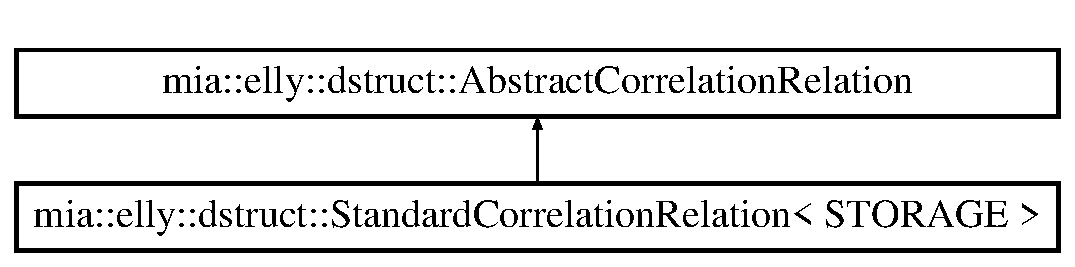
\includegraphics[height=2.000000cm]{classmia_1_1elly_1_1dstruct_1_1_standard_correlation_relation}
\end{center}
\end{figure}
\subsection*{Public Member Functions}
\begin{DoxyCompactItemize}
\item 
void $\ast$ \hyperlink{classmia_1_1elly_1_1dstruct_1_1_standard_correlation_relation_a0dfecae5ae55c35f407fc9fb44c216b0}{lookup} (int fid)
\item 
void \hyperlink{classmia_1_1elly_1_1dstruct_1_1_standard_correlation_relation_a8f71e78c27dabff352a2ec8bb532b82e}{update} (int fid, void($\ast$func\-\_\-update)(void $\ast$, int, int, int), int vid, int from, int to, bool \hyperlink{classmia_1_1elly_1_1dstruct_1_1_abstract_correlation_relation_a3291f1afe2252b5bc97414a96c035505}{lock})
\item 
void \hyperlink{classmia_1_1elly_1_1dstruct_1_1_standard_correlation_relation_ab6c7a97c05bca478980248a7dc466a02}{prepare} ()
\end{DoxyCompactItemize}
\subsection*{Public Attributes}
\begin{DoxyCompactItemize}
\item 
\hyperlink{classmia_1_1sm_1_1_key_value__vl}{mia\-::sm\-::\-Key\-Value\-\_\-vl}$<$ B\-U\-F\-F\-E\-R $>$ \hyperlink{classmia_1_1elly_1_1dstruct_1_1_standard_correlation_relation_a2648351b09b9c655802691f8e1c61cfb}{kv}
\end{DoxyCompactItemize}


\subsection{Detailed Description}
\subsubsection*{template$<$template$<$ template$<$ class C $>$ class A, class B $>$ class B\-U\-F\-F\-E\-R$>$class mia\-::elly\-::dstruct\-::\-Standard\-Correlation\-Relation$<$ B\-U\-F\-F\-E\-R $>$}

Correlation relation in which each factor contains a list of variable I\-Ds


\begin{DoxyTemplParams}{Template Parameters}
{\em B\-U\-F\-F\-E\-R} & Buffer to use for this correlation relation. \\
\hline
\end{DoxyTemplParams}


\subsection{Member Function Documentation}
\hypertarget{classmia_1_1elly_1_1dstruct_1_1_standard_correlation_relation_a0dfecae5ae55c35f407fc9fb44c216b0}{\index{mia\-::elly\-::dstruct\-::\-Standard\-Correlation\-Relation@{mia\-::elly\-::dstruct\-::\-Standard\-Correlation\-Relation}!lookup@{lookup}}
\index{lookup@{lookup}!mia::elly::dstruct::StandardCorrelationRelation@{mia\-::elly\-::dstruct\-::\-Standard\-Correlation\-Relation}}
\subsubsection[{lookup}]{\setlength{\rightskip}{0pt plus 5cm}template$<$template$<$ template$<$ class C $>$ class A, class B $>$ class B\-U\-F\-F\-E\-R$>$ void$\ast$ {\bf mia\-::elly\-::dstruct\-::\-Standard\-Correlation\-Relation}$<$ B\-U\-F\-F\-E\-R $>$\-::lookup (
\begin{DoxyParamCaption}
\item[{int}]{fid}
\end{DoxyParamCaption}
)\hspace{0.3cm}{\ttfamily [inline]}, {\ttfamily [virtual]}}}\label{classmia_1_1elly_1_1dstruct_1_1_standard_correlation_relation_a0dfecae5ae55c35f407fc9fb44c216b0}
Given a factor state I\-D, returns the pointer to V\-I\-D block.


\begin{DoxyParams}{Parameters}
{\em fid} & factor state I\-D.\\
\hline
\end{DoxyParams}
\begin{DoxyReturn}{Returns}
pointer to V\-I\-D block. 
\end{DoxyReturn}


Implements \hyperlink{classmia_1_1elly_1_1dstruct_1_1_abstract_correlation_relation}{mia\-::elly\-::dstruct\-::\-Abstract\-Correlation\-Relation}.

\hypertarget{classmia_1_1elly_1_1dstruct_1_1_standard_correlation_relation_ab6c7a97c05bca478980248a7dc466a02}{\index{mia\-::elly\-::dstruct\-::\-Standard\-Correlation\-Relation@{mia\-::elly\-::dstruct\-::\-Standard\-Correlation\-Relation}!prepare@{prepare}}
\index{prepare@{prepare}!mia::elly::dstruct::StandardCorrelationRelation@{mia\-::elly\-::dstruct\-::\-Standard\-Correlation\-Relation}}
\subsubsection[{prepare}]{\setlength{\rightskip}{0pt plus 5cm}template$<$template$<$ template$<$ class C $>$ class A, class B $>$ class B\-U\-F\-F\-E\-R$>$ void {\bf mia\-::elly\-::dstruct\-::\-Standard\-Correlation\-Relation}$<$ B\-U\-F\-F\-E\-R $>$\-::prepare (
\begin{DoxyParamCaption}
{}
\end{DoxyParamCaption}
)\hspace{0.3cm}{\ttfamily [inline]}, {\ttfamily [virtual]}}}\label{classmia_1_1elly_1_1dstruct_1_1_standard_correlation_relation_ab6c7a97c05bca478980248a7dc466a02}
Load factor from file \hyperlink{classmia_1_1elly_1_1dstruct_1_1_abstract_correlation_relation_a21e302ad723c9e0c99eb81c5bc420779}{mia\-::elly\-::dstruct\-::\-Abstract\-Correlation\-Relation\-::filename}. This function will fill in \hyperlink{classmia_1_1elly_1_1dstruct_1_1_standard_correlation_relation_a2648351b09b9c655802691f8e1c61cfb}{mia\-::elly\-::dstruct\-::\-Standard\-Correlation\-Relation\-::kv}. 

Implements \hyperlink{classmia_1_1elly_1_1dstruct_1_1_abstract_correlation_relation}{mia\-::elly\-::dstruct\-::\-Abstract\-Correlation\-Relation}.

\hypertarget{classmia_1_1elly_1_1dstruct_1_1_standard_correlation_relation_a8f71e78c27dabff352a2ec8bb532b82e}{\index{mia\-::elly\-::dstruct\-::\-Standard\-Correlation\-Relation@{mia\-::elly\-::dstruct\-::\-Standard\-Correlation\-Relation}!update@{update}}
\index{update@{update}!mia::elly::dstruct::StandardCorrelationRelation@{mia\-::elly\-::dstruct\-::\-Standard\-Correlation\-Relation}}
\subsubsection[{update}]{\setlength{\rightskip}{0pt plus 5cm}template$<$template$<$ template$<$ class C $>$ class A, class B $>$ class B\-U\-F\-F\-E\-R$>$ void {\bf mia\-::elly\-::dstruct\-::\-Standard\-Correlation\-Relation}$<$ B\-U\-F\-F\-E\-R $>$\-::update (
\begin{DoxyParamCaption}
\item[{int}]{fid, }
\item[{void($\ast$)(void $\ast$, int, int, int)}]{func\-\_\-update, }
\item[{int}]{vid, }
\item[{int}]{from, }
\item[{int}]{to, }
\item[{bool}]{lock}
\end{DoxyParamCaption}
)\hspace{0.3cm}{\ttfamily [inline]}, {\ttfamily [virtual]}}}\label{classmia_1_1elly_1_1dstruct_1_1_standard_correlation_relation_a8f71e78c27dabff352a2ec8bb532b82e}
Update factor state -- empty for \hyperlink{classmia_1_1elly_1_1dstruct_1_1_standard_correlation_relation}{mia\-::elly\-::dstruct\-::\-Standard\-Correlation\-Relation}.

\begin{DoxySeeAlso}{See also}
\hyperlink{classmia_1_1elly_1_1dstruct_1_1_incremental_correlation_relation}{mia\-::elly\-::dstruct\-::\-Incremental\-Correlation\-Relation}. 
\end{DoxySeeAlso}


Implements \hyperlink{classmia_1_1elly_1_1dstruct_1_1_abstract_correlation_relation}{mia\-::elly\-::dstruct\-::\-Abstract\-Correlation\-Relation}.



\subsection{Member Data Documentation}
\hypertarget{classmia_1_1elly_1_1dstruct_1_1_standard_correlation_relation_a2648351b09b9c655802691f8e1c61cfb}{\index{mia\-::elly\-::dstruct\-::\-Standard\-Correlation\-Relation@{mia\-::elly\-::dstruct\-::\-Standard\-Correlation\-Relation}!kv@{kv}}
\index{kv@{kv}!mia::elly::dstruct::StandardCorrelationRelation@{mia\-::elly\-::dstruct\-::\-Standard\-Correlation\-Relation}}
\subsubsection[{kv}]{\setlength{\rightskip}{0pt plus 5cm}template$<$template$<$ template$<$ class C $>$ class A, class B $>$ class B\-U\-F\-F\-E\-R$>$ {\bf mia\-::sm\-::\-Key\-Value\-\_\-vl}$<$B\-U\-F\-F\-E\-R$>$ {\bf mia\-::elly\-::dstruct\-::\-Standard\-Correlation\-Relation}$<$ B\-U\-F\-F\-E\-R $>$\-::kv}}\label{classmia_1_1elly_1_1dstruct_1_1_standard_correlation_relation_a2648351b09b9c655802691f8e1c61cfb}
Key value store that maps factor\-I\-D to block of V\-I\-Ds.

\begin{DoxySeeAlso}{See also}
\hyperlink{classmia_1_1sm_1_1_key_value__vl}{mia\-::sm\-::\-Key\-Value\-\_\-vl} 
\end{DoxySeeAlso}


The documentation for this class was generated from the following file\-:\begin{DoxyCompactItemize}
\item 
elly/elly/dstruct/Standard\-Correlation\-Relation.\-h\end{DoxyCompactItemize}

\hypertarget{structtests}{\section{tests Struct Reference}
\label{structtests}\index{tests@{tests}}
}
\subsection*{Public Attributes}
\begin{DoxyCompactItemize}
\item 
\hypertarget{structtests_a9ffa3e71f2157cbff7e6e0bbe27a2a35}{int {\bfseries aaa}}\label{structtests_a9ffa3e71f2157cbff7e6e0bbe27a2a35}

\item 
\hypertarget{structtests_aade716ac35e449a5bc1b59ab6b5cb1d5}{float {\bfseries bbb}}\label{structtests_aade716ac35e449a5bc1b59ab6b5cb1d5}

\item 
\hypertarget{structtests_a94f5600f6a9c111e59ed97216bcd7c19}{bool {\bfseries ccc}}\label{structtests_a94f5600f6a9c111e59ed97216bcd7c19}

\end{DoxyCompactItemize}


The documentation for this struct was generated from the following file\-:\begin{DoxyCompactItemize}
\item 
storageman/storageman/main.\-cpp\end{DoxyCompactItemize}

\hypertarget{structtestss}{\section{testss Struct Reference}
\label{structtestss}\index{testss@{testss}}
}
\subsection*{Public Attributes}
\begin{DoxyCompactItemize}
\item 
\hypertarget{structtestss_ae916d1791f70d60e93ce69d8e05fe316}{int {\bfseries a}}\label{structtestss_ae916d1791f70d60e93ce69d8e05fe316}

\item 
\hypertarget{structtestss_a3e01b19d3e897747e8153f9bc5994fe5}{int {\bfseries b}}\label{structtestss_a3e01b19d3e897747e8153f9bc5994fe5}

\item 
\hypertarget{structtestss_a7ce28bf11e1e05ebd4876bf23d01d523}{\hyperlink{structtests}{tests} {\bfseries c}}\label{structtestss_a7ce28bf11e1e05ebd4876bf23d01d523}

\item 
\hypertarget{structtestss_aaf1c0ca6a5bbc166817293e9001f2d04}{float {\bfseries d}}\label{structtestss_aaf1c0ca6a5bbc166817293e9001f2d04}

\end{DoxyCompactItemize}


The documentation for this struct was generated from the following file\-:\begin{DoxyCompactItemize}
\item 
/\-Users/czhang/\-Desktop/\-Codes/mia/src/storageman\-\_\-old/storageman/main.\-cpp\end{DoxyCompactItemize}

\hypertarget{classmia_1_1elly_1_1utils_1_1_timer}{\section{mia\-:\-:elly\-:\-:utils\-:\-:Timer Class Reference}
\label{classmia_1_1elly_1_1utils_1_1_timer}\index{mia\-::elly\-::utils\-::\-Timer@{mia\-::elly\-::utils\-::\-Timer}}
}
\subsection*{Public Member Functions}
\begin{DoxyCompactItemize}
\item 
\hypertarget{classmia_1_1elly_1_1utils_1_1_timer_ab1d1c1ad1f3a3931f9e83917494d4417}{void {\bfseries restart} ()}\label{classmia_1_1elly_1_1utils_1_1_timer_ab1d1c1ad1f3a3931f9e83917494d4417}

\item 
\hypertarget{classmia_1_1elly_1_1utils_1_1_timer_adbdb379b3e084eb86b88e5edaaefc27c}{float {\bfseries elapsed} ()}\label{classmia_1_1elly_1_1utils_1_1_timer_adbdb379b3e084eb86b88e5edaaefc27c}

\end{DoxyCompactItemize}
\subsection*{Public Attributes}
\begin{DoxyCompactItemize}
\item 
\hypertarget{classmia_1_1elly_1_1utils_1_1_timer_a2719cf47fab1edb158bf7a7424fed6af}{struct timespec {\bfseries \-\_\-start}}\label{classmia_1_1elly_1_1utils_1_1_timer_a2719cf47fab1edb158bf7a7424fed6af}

\item 
\hypertarget{classmia_1_1elly_1_1utils_1_1_timer_a04fc3f2bb34cc79d9761e23f4118d590}{struct timespec {\bfseries \-\_\-end}}\label{classmia_1_1elly_1_1utils_1_1_timer_a04fc3f2bb34cc79d9761e23f4118d590}

\end{DoxyCompactItemize}


The documentation for this class was generated from the following file\-:\begin{DoxyCompactItemize}
\item 
/\-Users/czhang/\-Desktop/\-Codes/mia/src/elly/elly/utils/Timer.\-h\end{DoxyCompactItemize}

\hypertarget{classmia_1_1sm_1_1_uniform_page}{\section{mia\-:\-:sm\-:\-:Uniform\-Page$<$ T\-Y\-P\-E $>$ Class Template Reference}
\label{classmia_1_1sm_1_1_uniform_page}\index{mia\-::sm\-::\-Uniform\-Page$<$ T\-Y\-P\-E $>$@{mia\-::sm\-::\-Uniform\-Page$<$ T\-Y\-P\-E $>$}}
}
\subsection*{Public Member Functions}
\begin{DoxyCompactItemize}
\item 
\hypertarget{classmia_1_1sm_1_1_uniform_page_a40192fe8c4807d001b501f12ece71726}{int {\bfseries push} (T\-Y\-P\-E obj)}\label{classmia_1_1sm_1_1_uniform_page_a40192fe8c4807d001b501f12ece71726}

\item 
\hypertarget{classmia_1_1sm_1_1_uniform_page_a1b4d3b4d6da50af483ecc12c9db752e1}{int {\bfseries get\-N\-Slot} ()}\label{classmia_1_1sm_1_1_uniform_page_a1b4d3b4d6da50af483ecc12c9db752e1}

\item 
\hypertarget{classmia_1_1sm_1_1_uniform_page_a4564403c3e09a938039b40664cab9889}{T\-Y\-P\-E {\bfseries get} (int nslot)}\label{classmia_1_1sm_1_1_uniform_page_a4564403c3e09a938039b40664cab9889}

\item 
\hypertarget{classmia_1_1sm_1_1_uniform_page_a3d88ab95f4dd9758fe4dd77cc2b25fa1}{void {\bfseries inplace\-\_\-update} (int nslot, T\-Y\-P\-E obj)}\label{classmia_1_1sm_1_1_uniform_page_a3d88ab95f4dd9758fe4dd77cc2b25fa1}

\end{DoxyCompactItemize}
\subsection*{Public Attributes}
\begin{DoxyCompactItemize}
\item 
\hypertarget{classmia_1_1sm_1_1_uniform_page_ac8ded3984b8229ce43107757fa65b1b3}{int {\bfseries Page\-N\-O\-B\-J}}\label{classmia_1_1sm_1_1_uniform_page_ac8ded3984b8229ce43107757fa65b1b3}

\item 
\hypertarget{classmia_1_1sm_1_1_uniform_page_a8800bc6de11955973a08647a7f594a26}{int {\bfseries cobj}}\label{classmia_1_1sm_1_1_uniform_page_a8800bc6de11955973a08647a7f594a26}

\item 
\hypertarget{classmia_1_1sm_1_1_uniform_page_a3a9679234f5ab08fd13ebd13f1df8def}{T\-Y\-P\-E {\bfseries content} \mbox{[}(Page\-S\-I\-Z\-E-\/8)/S\-I\-Z\-E\-O\-F(T\-Y\-P\-E)\mbox{]}}\label{classmia_1_1sm_1_1_uniform_page_a3a9679234f5ab08fd13ebd13f1df8def}

\item 
\hypertarget{classmia_1_1sm_1_1_uniform_page_a6fa558e53ca096e2ed7eaa1ee6eafde7}{bool {\bfseries align\-To\-Page\-Size} \mbox{[}(Page\-S\-I\-Z\-E-\/((int)(Page\-S\-I\-Z\-E-\/8)/S\-I\-Z\-E\-O\-F(T\-Y\-P\-E))$\ast$S\-I\-Z\-E\-O\-F(T\-Y\-P\-E)-\/8)\mbox{]}}\label{classmia_1_1sm_1_1_uniform_page_a6fa558e53ca096e2ed7eaa1ee6eafde7}

\end{DoxyCompactItemize}


The documentation for this class was generated from the following file\-:\begin{DoxyCompactItemize}
\item 
storageman/storageman/Uniform\-Page.\-h\end{DoxyCompactItemize}

\hypertarget{classmia_1_1elly_1_1dstruct_1_1_variable_assignment_relation}{\section{mia\-:\-:elly\-:\-:dstruct\-:\-:Variable\-Assignment\-Relation Class Reference}
\label{classmia_1_1elly_1_1dstruct_1_1_variable_assignment_relation}\index{mia\-::elly\-::dstruct\-::\-Variable\-Assignment\-Relation@{mia\-::elly\-::dstruct\-::\-Variable\-Assignment\-Relation}}
}


Variable assignment relation, which maps V\-I\-D to its current assignment.  




{\ttfamily \#include $<$Variable\-Assignment\-Relation.\-h$>$}

\subsection*{Public Member Functions}
\begin{DoxyCompactItemize}
\item 
int \hyperlink{classmia_1_1elly_1_1dstruct_1_1_variable_assignment_relation_adae435f1b7fe6ccbf4857d3a19a0f88a}{lookup} (int vid)
\item 
int \hyperlink{classmia_1_1elly_1_1dstruct_1_1_variable_assignment_relation_ad8c41e6f6a09c0fa5bb7e01b48e49875}{lookup\-\_\-domain} (int vid)
\item 
void \hyperlink{classmia_1_1elly_1_1dstruct_1_1_variable_assignment_relation_a226adad0ad27177aeeda5df1f0064290}{set} (int vid, int value)
\item 
void \hyperlink{classmia_1_1elly_1_1dstruct_1_1_variable_assignment_relation_a745e2d0883b72b0b2140bbd0b791b0d2}{prepare} ()
\end{DoxyCompactItemize}
\subsection*{Public Attributes}
\begin{DoxyCompactItemize}
\item 
std\-::string \hyperlink{classmia_1_1elly_1_1dstruct_1_1_variable_assignment_relation_aa48ef4351b3b43eaa3323cb20abb3531}{filename}
\item 
std\-::string \hyperlink{classmia_1_1elly_1_1dstruct_1_1_variable_assignment_relation_a52e11bd663360277cfc7c7be61d79990}{filetype}
\item 
\hyperlink{classmia_1_1sm_1_1_k_v}{mia\-::sm\-::\-K\-V}$<$ int, int, \\*
mia\-::sm\-::\-M\-M, mia\-::sm\-::\-D\-I\-R\-E\-C\-T, \\*
mia\-::sm\-::\-N\-I\-L, \\*
mia\-::sm\-::\-D\-E\-N\-S\-E\-\_\-\-K\-E\-Y $>$ \hyperlink{classmia_1_1elly_1_1dstruct_1_1_variable_assignment_relation_a1af337a9c0dcbd5fd8413c45df023017}{kf}
\item 
\hyperlink{classmia_1_1sm_1_1_k_v}{mia\-::sm\-::\-K\-V}$<$ int, int, \\*
mia\-::sm\-::\-M\-M, mia\-::sm\-::\-D\-I\-R\-E\-C\-T, \\*
mia\-::sm\-::\-N\-I\-L, \\*
mia\-::sm\-::\-D\-E\-N\-S\-E\-\_\-\-K\-E\-Y $>$ \hyperlink{classmia_1_1elly_1_1dstruct_1_1_variable_assignment_relation_ad26195bd52815d772770a07d65d755f5}{kf\-\_\-domain}
\item 
int \hyperlink{classmia_1_1elly_1_1dstruct_1_1_variable_assignment_relation_ad2dca4f9ea916afc044726130e6f8312}{nvariable}
\end{DoxyCompactItemize}


\subsection{Detailed Description}
Variable assignment relation, which maps V\-I\-D to its current assignment. 

\subsection{Member Function Documentation}
\hypertarget{classmia_1_1elly_1_1dstruct_1_1_variable_assignment_relation_adae435f1b7fe6ccbf4857d3a19a0f88a}{\index{mia\-::elly\-::dstruct\-::\-Variable\-Assignment\-Relation@{mia\-::elly\-::dstruct\-::\-Variable\-Assignment\-Relation}!lookup@{lookup}}
\index{lookup@{lookup}!mia::elly::dstruct::VariableAssignmentRelation@{mia\-::elly\-::dstruct\-::\-Variable\-Assignment\-Relation}}
\subsubsection[{lookup}]{\setlength{\rightskip}{0pt plus 5cm}int mia\-::elly\-::dstruct\-::\-Variable\-Assignment\-Relation\-::lookup (
\begin{DoxyParamCaption}
\item[{int}]{vid}
\end{DoxyParamCaption}
)\hspace{0.3cm}{\ttfamily [inline]}}}\label{classmia_1_1elly_1_1dstruct_1_1_variable_assignment_relation_adae435f1b7fe6ccbf4857d3a19a0f88a}
Given a variable I\-D, get its current assignment. \hypertarget{classmia_1_1elly_1_1dstruct_1_1_variable_assignment_relation_ad8c41e6f6a09c0fa5bb7e01b48e49875}{\index{mia\-::elly\-::dstruct\-::\-Variable\-Assignment\-Relation@{mia\-::elly\-::dstruct\-::\-Variable\-Assignment\-Relation}!lookup\-\_\-domain@{lookup\-\_\-domain}}
\index{lookup\-\_\-domain@{lookup\-\_\-domain}!mia::elly::dstruct::VariableAssignmentRelation@{mia\-::elly\-::dstruct\-::\-Variable\-Assignment\-Relation}}
\subsubsection[{lookup\-\_\-domain}]{\setlength{\rightskip}{0pt plus 5cm}int mia\-::elly\-::dstruct\-::\-Variable\-Assignment\-Relation\-::lookup\-\_\-domain (
\begin{DoxyParamCaption}
\item[{int}]{vid}
\end{DoxyParamCaption}
)\hspace{0.3cm}{\ttfamily [inline]}}}\label{classmia_1_1elly_1_1dstruct_1_1_variable_assignment_relation_ad8c41e6f6a09c0fa5bb7e01b48e49875}
Given a variable I\-D, get its domain. \hypertarget{classmia_1_1elly_1_1dstruct_1_1_variable_assignment_relation_a745e2d0883b72b0b2140bbd0b791b0d2}{\index{mia\-::elly\-::dstruct\-::\-Variable\-Assignment\-Relation@{mia\-::elly\-::dstruct\-::\-Variable\-Assignment\-Relation}!prepare@{prepare}}
\index{prepare@{prepare}!mia::elly::dstruct::VariableAssignmentRelation@{mia\-::elly\-::dstruct\-::\-Variable\-Assignment\-Relation}}
\subsubsection[{prepare}]{\setlength{\rightskip}{0pt plus 5cm}void mia\-::elly\-::dstruct\-::\-Variable\-Assignment\-Relation\-::prepare (
\begin{DoxyParamCaption}
{}
\end{DoxyParamCaption}
)\hspace{0.3cm}{\ttfamily [inline]}}}\label{classmia_1_1elly_1_1dstruct_1_1_variable_assignment_relation_a745e2d0883b72b0b2140bbd0b791b0d2}
Load file filename. \hypertarget{classmia_1_1elly_1_1dstruct_1_1_variable_assignment_relation_a226adad0ad27177aeeda5df1f0064290}{\index{mia\-::elly\-::dstruct\-::\-Variable\-Assignment\-Relation@{mia\-::elly\-::dstruct\-::\-Variable\-Assignment\-Relation}!set@{set}}
\index{set@{set}!mia::elly::dstruct::VariableAssignmentRelation@{mia\-::elly\-::dstruct\-::\-Variable\-Assignment\-Relation}}
\subsubsection[{set}]{\setlength{\rightskip}{0pt plus 5cm}void mia\-::elly\-::dstruct\-::\-Variable\-Assignment\-Relation\-::set (
\begin{DoxyParamCaption}
\item[{int}]{vid, }
\item[{int}]{value}
\end{DoxyParamCaption}
)\hspace{0.3cm}{\ttfamily [inline]}}}\label{classmia_1_1elly_1_1dstruct_1_1_variable_assignment_relation_a226adad0ad27177aeeda5df1f0064290}
Given a variable I\-D and a new value, update the key value store. 

\subsection{Member Data Documentation}
\hypertarget{classmia_1_1elly_1_1dstruct_1_1_variable_assignment_relation_aa48ef4351b3b43eaa3323cb20abb3531}{\index{mia\-::elly\-::dstruct\-::\-Variable\-Assignment\-Relation@{mia\-::elly\-::dstruct\-::\-Variable\-Assignment\-Relation}!filename@{filename}}
\index{filename@{filename}!mia::elly::dstruct::VariableAssignmentRelation@{mia\-::elly\-::dstruct\-::\-Variable\-Assignment\-Relation}}
\subsubsection[{filename}]{\setlength{\rightskip}{0pt plus 5cm}std\-::string mia\-::elly\-::dstruct\-::\-Variable\-Assignment\-Relation\-::filename}}\label{classmia_1_1elly_1_1dstruct_1_1_variable_assignment_relation_aa48ef4351b3b43eaa3323cb20abb3531}
\-\_\-\-\_\-vf.\-tsv file's path, which contains the domain of each variable. \hypertarget{classmia_1_1elly_1_1dstruct_1_1_variable_assignment_relation_a52e11bd663360277cfc7c7be61d79990}{\index{mia\-::elly\-::dstruct\-::\-Variable\-Assignment\-Relation@{mia\-::elly\-::dstruct\-::\-Variable\-Assignment\-Relation}!filetype@{filetype}}
\index{filetype@{filetype}!mia::elly::dstruct::VariableAssignmentRelation@{mia\-::elly\-::dstruct\-::\-Variable\-Assignment\-Relation}}
\subsubsection[{filetype}]{\setlength{\rightskip}{0pt plus 5cm}std\-::string mia\-::elly\-::dstruct\-::\-Variable\-Assignment\-Relation\-::filetype}}\label{classmia_1_1elly_1_1dstruct_1_1_variable_assignment_relation_a52e11bd663360277cfc7c7be61d79990}
Type of input file. \{tsv\} \hypertarget{classmia_1_1elly_1_1dstruct_1_1_variable_assignment_relation_a1af337a9c0dcbd5fd8413c45df023017}{\index{mia\-::elly\-::dstruct\-::\-Variable\-Assignment\-Relation@{mia\-::elly\-::dstruct\-::\-Variable\-Assignment\-Relation}!kf@{kf}}
\index{kf@{kf}!mia::elly::dstruct::VariableAssignmentRelation@{mia\-::elly\-::dstruct\-::\-Variable\-Assignment\-Relation}}
\subsubsection[{kf}]{\setlength{\rightskip}{0pt plus 5cm}{\bf mia\-::sm\-::\-K\-V}$<$int, int, mia\-::sm\-::\-M\-M, mia\-::sm\-::\-D\-I\-R\-E\-C\-T, mia\-::sm\-::\-N\-I\-L, mia\-::sm\-::\-D\-E\-N\-S\-E\-\_\-\-K\-E\-Y$>$ mia\-::elly\-::dstruct\-::\-Variable\-Assignment\-Relation\-::kf}}\label{classmia_1_1elly_1_1dstruct_1_1_variable_assignment_relation_a1af337a9c0dcbd5fd8413c45df023017}
Key value store which maps V\-I\-D to its assignment. \hypertarget{classmia_1_1elly_1_1dstruct_1_1_variable_assignment_relation_ad26195bd52815d772770a07d65d755f5}{\index{mia\-::elly\-::dstruct\-::\-Variable\-Assignment\-Relation@{mia\-::elly\-::dstruct\-::\-Variable\-Assignment\-Relation}!kf\-\_\-domain@{kf\-\_\-domain}}
\index{kf\-\_\-domain@{kf\-\_\-domain}!mia::elly::dstruct::VariableAssignmentRelation@{mia\-::elly\-::dstruct\-::\-Variable\-Assignment\-Relation}}
\subsubsection[{kf\-\_\-domain}]{\setlength{\rightskip}{0pt plus 5cm}{\bf mia\-::sm\-::\-K\-V}$<$int, int, mia\-::sm\-::\-M\-M, mia\-::sm\-::\-D\-I\-R\-E\-C\-T, mia\-::sm\-::\-N\-I\-L, mia\-::sm\-::\-D\-E\-N\-S\-E\-\_\-\-K\-E\-Y$>$ mia\-::elly\-::dstruct\-::\-Variable\-Assignment\-Relation\-::kf\-\_\-domain}}\label{classmia_1_1elly_1_1dstruct_1_1_variable_assignment_relation_ad26195bd52815d772770a07d65d755f5}
Key value store which maps V\-I\-D to its domain. \hypertarget{classmia_1_1elly_1_1dstruct_1_1_variable_assignment_relation_ad2dca4f9ea916afc044726130e6f8312}{\index{mia\-::elly\-::dstruct\-::\-Variable\-Assignment\-Relation@{mia\-::elly\-::dstruct\-::\-Variable\-Assignment\-Relation}!nvariable@{nvariable}}
\index{nvariable@{nvariable}!mia::elly::dstruct::VariableAssignmentRelation@{mia\-::elly\-::dstruct\-::\-Variable\-Assignment\-Relation}}
\subsubsection[{nvariable}]{\setlength{\rightskip}{0pt plus 5cm}int mia\-::elly\-::dstruct\-::\-Variable\-Assignment\-Relation\-::nvariable}}\label{classmia_1_1elly_1_1dstruct_1_1_variable_assignment_relation_ad2dca4f9ea916afc044726130e6f8312}
Number of variables being loaded. 

The documentation for this class was generated from the following file\-:\begin{DoxyCompactItemize}
\item 
/\-Users/czhang/\-Desktop/\-Codes/mia/src/elly/elly/dstruct/Variable\-Assignment\-Relation.\-h\end{DoxyCompactItemize}

\hypertarget{classmia_1_1elly_1_1dstruct_1_1_variable_factor_relation}{\section{mia\-:\-:elly\-:\-:dstruct\-:\-:Variable\-Factor\-Relation Class Reference}
\label{classmia_1_1elly_1_1dstruct_1_1_variable_factor_relation}\index{mia\-::elly\-::dstruct\-::\-Variable\-Factor\-Relation@{mia\-::elly\-::dstruct\-::\-Variable\-Factor\-Relation}}
}


Variable factor relation which maps each variable to the set of factors.  




{\ttfamily \#include $<$Variable\-Factor\-Relation.\-h$>$}

\subsection*{Public Member Functions}
\begin{DoxyCompactItemize}
\item 
\hyperlink{classmia_1_1sm_1_1_ints_block}{mia\-::sm\-::\-Ints\-Block} \hyperlink{classmia_1_1elly_1_1dstruct_1_1_variable_factor_relation_a6f3b93d27d11f688cfe9952f057d9a3f}{lookup} (int vid)
\item 
void \hyperlink{classmia_1_1elly_1_1dstruct_1_1_variable_factor_relation_aa264b71ee5c828e06b85cd3588262cf3}{prepare} ()
\end{DoxyCompactItemize}
\subsection*{Public Attributes}
\begin{DoxyCompactItemize}
\item 
std\-::string \hyperlink{classmia_1_1elly_1_1dstruct_1_1_variable_factor_relation_a582e0a5fb2699076d5ec719a32613129}{filename}
\item 
std\-::string \hyperlink{classmia_1_1elly_1_1dstruct_1_1_variable_factor_relation_a14811849a23c099c5d1d9abb718f3d9f}{filetype}
\item 
\hyperlink{classmia_1_1sm_1_1_k_v}{mia\-::sm\-::\-K\-V}$<$ int, \\*
\hyperlink{classmia_1_1sm_1_1_ints_block}{mia\-::sm\-::\-Ints\-Block}, \\*
mia\-::sm\-::\-M\-M\-A\-P, mia\-::sm\-::\-D\-I\-R\-E\-C\-T, \\*
mia\-::sm\-::\-N\-I\-L, \\*
mia\-::sm\-::\-D\-E\-N\-S\-E\-\_\-\-K\-E\-Y $>$ \hyperlink{classmia_1_1elly_1_1dstruct_1_1_variable_factor_relation_ac009b6fd58e9f29f389e4c274abf1335}{kv}
\item 
int \hyperlink{classmia_1_1elly_1_1dstruct_1_1_variable_factor_relation_ac3f1f9186a88af83b82868b4077ccdc2}{nvariable}
\end{DoxyCompactItemize}


\subsection{Detailed Description}
Variable factor relation which maps each variable to the set of factors. 

\subsection{Member Function Documentation}
\hypertarget{classmia_1_1elly_1_1dstruct_1_1_variable_factor_relation_a6f3b93d27d11f688cfe9952f057d9a3f}{\index{mia\-::elly\-::dstruct\-::\-Variable\-Factor\-Relation@{mia\-::elly\-::dstruct\-::\-Variable\-Factor\-Relation}!lookup@{lookup}}
\index{lookup@{lookup}!mia::elly::dstruct::VariableFactorRelation@{mia\-::elly\-::dstruct\-::\-Variable\-Factor\-Relation}}
\subsubsection[{lookup}]{\setlength{\rightskip}{0pt plus 5cm}{\bf mia\-::sm\-::\-Ints\-Block} mia\-::elly\-::dstruct\-::\-Variable\-Factor\-Relation\-::lookup (
\begin{DoxyParamCaption}
\item[{int}]{vid}
\end{DoxyParamCaption}
)\hspace{0.3cm}{\ttfamily [inline]}}}\label{classmia_1_1elly_1_1dstruct_1_1_variable_factor_relation_a6f3b93d27d11f688cfe9952f057d9a3f}
Given a V\-I\-D, get factor block. \hypertarget{classmia_1_1elly_1_1dstruct_1_1_variable_factor_relation_aa264b71ee5c828e06b85cd3588262cf3}{\index{mia\-::elly\-::dstruct\-::\-Variable\-Factor\-Relation@{mia\-::elly\-::dstruct\-::\-Variable\-Factor\-Relation}!prepare@{prepare}}
\index{prepare@{prepare}!mia::elly::dstruct::VariableFactorRelation@{mia\-::elly\-::dstruct\-::\-Variable\-Factor\-Relation}}
\subsubsection[{prepare}]{\setlength{\rightskip}{0pt plus 5cm}void mia\-::elly\-::dstruct\-::\-Variable\-Factor\-Relation\-::prepare (
\begin{DoxyParamCaption}
{}
\end{DoxyParamCaption}
)\hspace{0.3cm}{\ttfamily [inline]}}}\label{classmia_1_1elly_1_1dstruct_1_1_variable_factor_relation_aa264b71ee5c828e06b85cd3588262cf3}
Load from file filename; 

\subsection{Member Data Documentation}
\hypertarget{classmia_1_1elly_1_1dstruct_1_1_variable_factor_relation_a582e0a5fb2699076d5ec719a32613129}{\index{mia\-::elly\-::dstruct\-::\-Variable\-Factor\-Relation@{mia\-::elly\-::dstruct\-::\-Variable\-Factor\-Relation}!filename@{filename}}
\index{filename@{filename}!mia::elly::dstruct::VariableFactorRelation@{mia\-::elly\-::dstruct\-::\-Variable\-Factor\-Relation}}
\subsubsection[{filename}]{\setlength{\rightskip}{0pt plus 5cm}std\-::string mia\-::elly\-::dstruct\-::\-Variable\-Factor\-Relation\-::filename}}\label{classmia_1_1elly_1_1dstruct_1_1_variable_factor_relation_a582e0a5fb2699076d5ec719a32613129}
\-\_\-\-\_\-vf file's path. \hypertarget{classmia_1_1elly_1_1dstruct_1_1_variable_factor_relation_a14811849a23c099c5d1d9abb718f3d9f}{\index{mia\-::elly\-::dstruct\-::\-Variable\-Factor\-Relation@{mia\-::elly\-::dstruct\-::\-Variable\-Factor\-Relation}!filetype@{filetype}}
\index{filetype@{filetype}!mia::elly::dstruct::VariableFactorRelation@{mia\-::elly\-::dstruct\-::\-Variable\-Factor\-Relation}}
\subsubsection[{filetype}]{\setlength{\rightskip}{0pt plus 5cm}std\-::string mia\-::elly\-::dstruct\-::\-Variable\-Factor\-Relation\-::filetype}}\label{classmia_1_1elly_1_1dstruct_1_1_variable_factor_relation_a14811849a23c099c5d1d9abb718f3d9f}
type of input file. \{tsv\} \hypertarget{classmia_1_1elly_1_1dstruct_1_1_variable_factor_relation_ac009b6fd58e9f29f389e4c274abf1335}{\index{mia\-::elly\-::dstruct\-::\-Variable\-Factor\-Relation@{mia\-::elly\-::dstruct\-::\-Variable\-Factor\-Relation}!kv@{kv}}
\index{kv@{kv}!mia::elly::dstruct::VariableFactorRelation@{mia\-::elly\-::dstruct\-::\-Variable\-Factor\-Relation}}
\subsubsection[{kv}]{\setlength{\rightskip}{0pt plus 5cm}{\bf mia\-::sm\-::\-K\-V}$<$int, {\bf mia\-::sm\-::\-Ints\-Block}, mia\-::sm\-::\-M\-M\-A\-P, mia\-::sm\-::\-D\-I\-R\-E\-C\-T, mia\-::sm\-::\-N\-I\-L, mia\-::sm\-::\-D\-E\-N\-S\-E\-\_\-\-K\-E\-Y$>$ mia\-::elly\-::dstruct\-::\-Variable\-Factor\-Relation\-::kv}}\label{classmia_1_1elly_1_1dstruct_1_1_variable_factor_relation_ac009b6fd58e9f29f389e4c274abf1335}
Key value store that maps V\-I\-D to factor block. \hypertarget{classmia_1_1elly_1_1dstruct_1_1_variable_factor_relation_ac3f1f9186a88af83b82868b4077ccdc2}{\index{mia\-::elly\-::dstruct\-::\-Variable\-Factor\-Relation@{mia\-::elly\-::dstruct\-::\-Variable\-Factor\-Relation}!nvariable@{nvariable}}
\index{nvariable@{nvariable}!mia::elly::dstruct::VariableFactorRelation@{mia\-::elly\-::dstruct\-::\-Variable\-Factor\-Relation}}
\subsubsection[{nvariable}]{\setlength{\rightskip}{0pt plus 5cm}int mia\-::elly\-::dstruct\-::\-Variable\-Factor\-Relation\-::nvariable}}\label{classmia_1_1elly_1_1dstruct_1_1_variable_factor_relation_ac3f1f9186a88af83b82868b4077ccdc2}
Number of vairables being loaded. 

The documentation for this class was generated from the following file\-:\begin{DoxyCompactItemize}
\item 
/\-Users/czhang/\-Desktop/\-Codes/mia/src/elly/elly/dstruct/Variable\-Factor\-Relation.\-h\end{DoxyCompactItemize}

\hypertarget{classmia_1_1elly_1_1dstruct_1_1_variable_tally_relation}{\section{mia\-:\-:elly\-:\-:dstruct\-:\-:Variable\-Tally\-Relation Class Reference}
\label{classmia_1_1elly_1_1dstruct_1_1_variable_tally_relation}\index{mia\-::elly\-::dstruct\-::\-Variable\-Tally\-Relation@{mia\-::elly\-::dstruct\-::\-Variable\-Tally\-Relation}}
}


Variable tally relation which maps a variable to the int block contains tally info.  




{\ttfamily \#include $<$Variable\-Tally\-Relation.\-h$>$}

\subsection*{Public Member Functions}
\begin{DoxyCompactItemize}
\item 
\hypertarget{classmia_1_1elly_1_1dstruct_1_1_variable_tally_relation_a9d181c38b6f5b0a00f9ae033ea9ca14b}{\hyperlink{classmia_1_1sm_1_1_ints_block}{mia\-::sm\-::\-Ints\-Block} {\bfseries lookup} (int vid)}\label{classmia_1_1elly_1_1dstruct_1_1_variable_tally_relation_a9d181c38b6f5b0a00f9ae033ea9ca14b}

\item 
\hypertarget{classmia_1_1elly_1_1dstruct_1_1_variable_tally_relation_a43fe583de7fae37ec40ba1f86a5a0a0c}{void {\bfseries tally} (int vid, int value)}\label{classmia_1_1elly_1_1dstruct_1_1_variable_tally_relation_a43fe583de7fae37ec40ba1f86a5a0a0c}

\item 
\hypertarget{classmia_1_1elly_1_1dstruct_1_1_variable_tally_relation_a9619f574476f63f659c93e4585a9df1f}{void {\bfseries prepare} ()}\label{classmia_1_1elly_1_1dstruct_1_1_variable_tally_relation_a9619f574476f63f659c93e4585a9df1f}

\end{DoxyCompactItemize}
\subsection*{Public Attributes}
\begin{DoxyCompactItemize}
\item 
\hypertarget{classmia_1_1elly_1_1dstruct_1_1_variable_tally_relation_a215fa9dcce3e8e1e6966187f6ec22fff}{std\-::string {\bfseries filename}}\label{classmia_1_1elly_1_1dstruct_1_1_variable_tally_relation_a215fa9dcce3e8e1e6966187f6ec22fff}

\item 
\hypertarget{classmia_1_1elly_1_1dstruct_1_1_variable_tally_relation_a352086250fc1f8190752fc6fb2695aa0}{std\-::string {\bfseries filetype}}\label{classmia_1_1elly_1_1dstruct_1_1_variable_tally_relation_a352086250fc1f8190752fc6fb2695aa0}

\item 
\hypertarget{classmia_1_1elly_1_1dstruct_1_1_variable_tally_relation_abd1e8a631336293a2799bd26e10f7ab5}{\hyperlink{classmia_1_1sm_1_1_k_v}{mia\-::sm\-::\-K\-V}$<$ int, \\*
\hyperlink{classmia_1_1sm_1_1_ints_block}{mia\-::sm\-::\-Ints\-Block}, \\*
mia\-::sm\-::\-M\-M, mia\-::sm\-::\-D\-I\-R\-E\-C\-T, \\*
mia\-::sm\-::\-N\-I\-L, \\*
mia\-::sm\-::\-D\-E\-N\-S\-E\-\_\-\-K\-E\-Y $>$ {\bfseries kv}}\label{classmia_1_1elly_1_1dstruct_1_1_variable_tally_relation_abd1e8a631336293a2799bd26e10f7ab5}

\item 
\hypertarget{classmia_1_1elly_1_1dstruct_1_1_variable_tally_relation_a1057afeffd94e72b1f7e1778ad0a268b}{int {\bfseries nvariable}}\label{classmia_1_1elly_1_1dstruct_1_1_variable_tally_relation_a1057afeffd94e72b1f7e1778ad0a268b}

\end{DoxyCompactItemize}


\subsection{Detailed Description}
Variable tally relation which maps a variable to the int block contains tally info. 

The documentation for this class was generated from the following file\-:\begin{DoxyCompactItemize}
\item 
/\-Users/czhang/\-Desktop/\-Codes/mia/src/elly/elly/dstruct/Variable\-Tally\-Relation.\-h\end{DoxyCompactItemize}

\hypertarget{classmia_1_1elly_1_1dstruct_1_1_variable_training_relation}{\section{mia\-:\-:elly\-:\-:dstruct\-:\-:Variable\-Training\-Relation Class Reference}
\label{classmia_1_1elly_1_1dstruct_1_1_variable_training_relation}\index{mia\-::elly\-::dstruct\-::\-Variable\-Training\-Relation@{mia\-::elly\-::dstruct\-::\-Variable\-Training\-Relation}}
}


Variable training relation which maps a variable to its value in training data.  




{\ttfamily \#include $<$Variable\-Training\-Relation.\-h$>$}

\subsection*{Public Member Functions}
\begin{DoxyCompactItemize}
\item 
\hypertarget{classmia_1_1elly_1_1dstruct_1_1_variable_training_relation_a9cb4f20019182911637db8a593a85fbd}{int {\bfseries lookup} (int vid)}\label{classmia_1_1elly_1_1dstruct_1_1_variable_training_relation_a9cb4f20019182911637db8a593a85fbd}

\item 
\hypertarget{classmia_1_1elly_1_1dstruct_1_1_variable_training_relation_ac77cbc07585f81a6e02a49bb56baeba7}{void {\bfseries prepare} ()}\label{classmia_1_1elly_1_1dstruct_1_1_variable_training_relation_ac77cbc07585f81a6e02a49bb56baeba7}

\end{DoxyCompactItemize}
\subsection*{Public Attributes}
\begin{DoxyCompactItemize}
\item 
\hypertarget{classmia_1_1elly_1_1dstruct_1_1_variable_training_relation_a21a386fd538d32997490bfdfaf16e89c}{std\-::string {\bfseries filename}}\label{classmia_1_1elly_1_1dstruct_1_1_variable_training_relation_a21a386fd538d32997490bfdfaf16e89c}

\item 
\hypertarget{classmia_1_1elly_1_1dstruct_1_1_variable_training_relation_a9a73ac31be32e3f0cc18785c841e78c1}{std\-::string {\bfseries filetype}}\label{classmia_1_1elly_1_1dstruct_1_1_variable_training_relation_a9a73ac31be32e3f0cc18785c841e78c1}

\item 
\hypertarget{classmia_1_1elly_1_1dstruct_1_1_variable_training_relation_adf9ee27ce1d35a996a2b01ae8251cb79}{\hyperlink{classmia_1_1sm_1_1_k_v}{mia\-::sm\-::\-K\-V}$<$ int, int, \\*
mia\-::sm\-::\-M\-M, mia\-::sm\-::\-D\-I\-R\-E\-C\-T, \\*
mia\-::sm\-::\-N\-I\-L, \\*
mia\-::sm\-::\-D\-E\-N\-S\-E\-\_\-\-K\-E\-Y $>$ {\bfseries kv}}\label{classmia_1_1elly_1_1dstruct_1_1_variable_training_relation_adf9ee27ce1d35a996a2b01ae8251cb79}

\item 
\hypertarget{classmia_1_1elly_1_1dstruct_1_1_variable_training_relation_ac651af7167f73bfbc51fa6c940562d52}{int {\bfseries nvariable}}\label{classmia_1_1elly_1_1dstruct_1_1_variable_training_relation_ac651af7167f73bfbc51fa6c940562d52}

\end{DoxyCompactItemize}


\subsection{Detailed Description}
Variable training relation which maps a variable to its value in training data. 

The documentation for this class was generated from the following file\-:\begin{DoxyCompactItemize}
\item 
/\-Users/czhang/\-Desktop/\-Codes/mia/src/elly/elly/dstruct/Variable\-Training\-Relation.\-h\end{DoxyCompactItemize}

\printindex
\end{document}
